\documentclass[]{article}
\usepackage{lmodern}
\usepackage{amssymb,amsmath}
\usepackage{ifxetex,ifluatex}
\usepackage{fixltx2e} % provides \textsubscript
\ifnum 0\ifxetex 1\fi\ifluatex 1\fi=0 % if pdftex
  \usepackage[T1]{fontenc}
  \usepackage[utf8]{inputenc}
\else % if luatex or xelatex
  \ifxetex
    \usepackage{mathspec}
  \else
    \usepackage{fontspec}
  \fi
  \defaultfontfeatures{Ligatures=TeX,Scale=MatchLowercase}
\fi
% use upquote if available, for straight quotes in verbatim environments
\IfFileExists{upquote.sty}{\usepackage{upquote}}{}
% use microtype if available
\IfFileExists{microtype.sty}{%
\usepackage{microtype}
\UseMicrotypeSet[protrusion]{basicmath} % disable protrusion for tt fonts
}{}
\usepackage[margin=1in]{geometry}
\usepackage{hyperref}
\hypersetup{unicode=true,
            pdftitle={Titanic Data Clean},
            pdfauthor={Ricardo Garcia Ruiz},
            pdfborder={0 0 0},
            breaklinks=true}
\urlstyle{same}  % don't use monospace font for urls
\usepackage{color}
\usepackage{fancyvrb}
\newcommand{\VerbBar}{|}
\newcommand{\VERB}{\Verb[commandchars=\\\{\}]}
\DefineVerbatimEnvironment{Highlighting}{Verbatim}{commandchars=\\\{\}}
% Add ',fontsize=\small' for more characters per line
\usepackage{framed}
\definecolor{shadecolor}{RGB}{248,248,248}
\newenvironment{Shaded}{\begin{snugshade}}{\end{snugshade}}
\newcommand{\KeywordTok}[1]{\textcolor[rgb]{0.13,0.29,0.53}{\textbf{#1}}}
\newcommand{\DataTypeTok}[1]{\textcolor[rgb]{0.13,0.29,0.53}{#1}}
\newcommand{\DecValTok}[1]{\textcolor[rgb]{0.00,0.00,0.81}{#1}}
\newcommand{\BaseNTok}[1]{\textcolor[rgb]{0.00,0.00,0.81}{#1}}
\newcommand{\FloatTok}[1]{\textcolor[rgb]{0.00,0.00,0.81}{#1}}
\newcommand{\ConstantTok}[1]{\textcolor[rgb]{0.00,0.00,0.00}{#1}}
\newcommand{\CharTok}[1]{\textcolor[rgb]{0.31,0.60,0.02}{#1}}
\newcommand{\SpecialCharTok}[1]{\textcolor[rgb]{0.00,0.00,0.00}{#1}}
\newcommand{\StringTok}[1]{\textcolor[rgb]{0.31,0.60,0.02}{#1}}
\newcommand{\VerbatimStringTok}[1]{\textcolor[rgb]{0.31,0.60,0.02}{#1}}
\newcommand{\SpecialStringTok}[1]{\textcolor[rgb]{0.31,0.60,0.02}{#1}}
\newcommand{\ImportTok}[1]{#1}
\newcommand{\CommentTok}[1]{\textcolor[rgb]{0.56,0.35,0.01}{\textit{#1}}}
\newcommand{\DocumentationTok}[1]{\textcolor[rgb]{0.56,0.35,0.01}{\textbf{\textit{#1}}}}
\newcommand{\AnnotationTok}[1]{\textcolor[rgb]{0.56,0.35,0.01}{\textbf{\textit{#1}}}}
\newcommand{\CommentVarTok}[1]{\textcolor[rgb]{0.56,0.35,0.01}{\textbf{\textit{#1}}}}
\newcommand{\OtherTok}[1]{\textcolor[rgb]{0.56,0.35,0.01}{#1}}
\newcommand{\FunctionTok}[1]{\textcolor[rgb]{0.00,0.00,0.00}{#1}}
\newcommand{\VariableTok}[1]{\textcolor[rgb]{0.00,0.00,0.00}{#1}}
\newcommand{\ControlFlowTok}[1]{\textcolor[rgb]{0.13,0.29,0.53}{\textbf{#1}}}
\newcommand{\OperatorTok}[1]{\textcolor[rgb]{0.81,0.36,0.00}{\textbf{#1}}}
\newcommand{\BuiltInTok}[1]{#1}
\newcommand{\ExtensionTok}[1]{#1}
\newcommand{\PreprocessorTok}[1]{\textcolor[rgb]{0.56,0.35,0.01}{\textit{#1}}}
\newcommand{\AttributeTok}[1]{\textcolor[rgb]{0.77,0.63,0.00}{#1}}
\newcommand{\RegionMarkerTok}[1]{#1}
\newcommand{\InformationTok}[1]{\textcolor[rgb]{0.56,0.35,0.01}{\textbf{\textit{#1}}}}
\newcommand{\WarningTok}[1]{\textcolor[rgb]{0.56,0.35,0.01}{\textbf{\textit{#1}}}}
\newcommand{\AlertTok}[1]{\textcolor[rgb]{0.94,0.16,0.16}{#1}}
\newcommand{\ErrorTok}[1]{\textcolor[rgb]{0.64,0.00,0.00}{\textbf{#1}}}
\newcommand{\NormalTok}[1]{#1}
\usepackage{longtable,booktabs}
\usepackage{graphicx,grffile}
\makeatletter
\def\maxwidth{\ifdim\Gin@nat@width>\linewidth\linewidth\else\Gin@nat@width\fi}
\def\maxheight{\ifdim\Gin@nat@height>\textheight\textheight\else\Gin@nat@height\fi}
\makeatother
% Scale images if necessary, so that they will not overflow the page
% margins by default, and it is still possible to overwrite the defaults
% using explicit options in \includegraphics[width, height, ...]{}
\setkeys{Gin}{width=\maxwidth,height=\maxheight,keepaspectratio}
\IfFileExists{parskip.sty}{%
\usepackage{parskip}
}{% else
\setlength{\parindent}{0pt}
\setlength{\parskip}{6pt plus 2pt minus 1pt}
}
\setlength{\emergencystretch}{3em}  % prevent overfull lines
\providecommand{\tightlist}{%
  \setlength{\itemsep}{0pt}\setlength{\parskip}{0pt}}
\setcounter{secnumdepth}{5}
% Redefines (sub)paragraphs to behave more like sections
\ifx\paragraph\undefined\else
\let\oldparagraph\paragraph
\renewcommand{\paragraph}[1]{\oldparagraph{#1}\mbox{}}
\fi
\ifx\subparagraph\undefined\else
\let\oldsubparagraph\subparagraph
\renewcommand{\subparagraph}[1]{\oldsubparagraph{#1}\mbox{}}
\fi

%%% Use protect on footnotes to avoid problems with footnotes in titles
\let\rmarkdownfootnote\footnote%
\def\footnote{\protect\rmarkdownfootnote}

%%% Change title format to be more compact
\usepackage{titling}

% Create subtitle command for use in maketitle
\newcommand{\subtitle}[1]{
  \posttitle{
    \begin{center}\large#1\end{center}
    }
}

\setlength{\droptitle}{-2em}
  \title{Titanic Data Clean}
  \pretitle{\vspace{\droptitle}\centering\huge}
  \posttitle{\par}
  \author{Ricardo Garcia Ruiz}
  \preauthor{\centering\large\emph}
  \postauthor{\par}
  \predate{\centering\large\emph}
  \postdate{\par}
  \date{9 de junio, 2018}


\begin{document}
\maketitle

{
\setcounter{tocdepth}{3}
\tableofcontents
}
\section{Práctica 2: Limpieza y validación de los
datos}\label{practica-2-limpieza-y-validacion-de-los-datos}

\subsection{Descripción de la Práctica a
realizar}\label{descripcion-de-la-practica-a-realizar}

El objetivo de esta actividad será el tratamiento de un dataset, que
puede ser el creado en la práctica 1 o bien cualquier dataset libre
disponible en Kaggle (\url{https://www.kaggle.com}). Algunos ejemplos de
dataset con los que podéis trabajar son: * Red Wine Quality
(\url{https://www.kaggle.com/uciml/red-wine-quality-cortez-et-al-2009})
* Titanic: Machine Learning from Disaster
(\url{https://www.kaggle.com/c/titanic}) * Predict Future Sales
(\url{https://www.kaggle.com/c/competitive-data-sciencepredict-future-sales/}).

Los últimos dos ejemplos corresponden a competiciones activas de Kaggle
de manera que, opcionalmente, podríais aprovechar el trabajo realizado
durante la práctica para entrar en alguna de estas competiciones.

Siguiendo las principales etapas de un proyecto analítico, las
diferentes tareas a realizar (y justificar) son las siguientes:

\begin{enumerate}
\def\labelenumi{\arabic{enumi}.}
\tightlist
\item
  Descripción del dataset. ¿Por qué es importante y qué
  pregunta/problema pretende responder?
\item
  Integración y selección de los datos de interés a analizar.
\item
  Limpieza de los datos:\\
  3.1. ¿Los datos contienen ceros o elementos vacíos? ¿Cómo gestionarías
  cada uno de estos casos? 3.2. Identificación y tratamiento de valores
  extremos.
\item
  Análisis de los datos.\\
  4.1. Selección de los grupos de datos que se quieren analizar/comparar
  (planificación de los análisis a aplicar).\\
  4.2. Comprobación de la normalidad y homogeneidad de la varianza.\\
  4.3. Aplicación de pruebas estadísticas para comparar los grupos de
  datos. En función de los datos y el objetivo del estudio, aplicar
  pruebas de contraste de hipótesis, correlaciones, regresiones, etc.
\item
  Representación de los resultados a partir de tablas y gráficas.
\item
  Resolución del problema. A partir de los resultados obtenidos, ¿cuáles
  son las conclusiones? ¿Los resultados permiten responder al problema?
\item
  Código: Hay que adjuntar el código, preferiblemente en R, con el que
  se ha realizado la limpieza, análisis y representación de los datos.
  Si lo preferís, también podéis trabajar en Python.
\end{enumerate}

\subsection{Objetivos}\label{objetivos}

Los objetivos concretos de esta práctica son:

\begin{itemize}
\tightlist
\item
  Aprender a aplicar los conocimientos adquiridos y su capacidad de
  resolución de problemas en entornos nuevos o poco conocidos dentro de
  contextos más amplios o multidisciplinares.\\
\item
  Saber identificar los datos relevantes y los tratamientos necesarios
  (integración, limpieza y validación) para llevar a cabo un proyecto
  analítico.\\
\item
  Aprender a analizar los datos adecuadamente para abordar la
  información contenida en los datos.\\
\item
  Identificar la mejor representación de los resultados para aportar
  conclusiones sobre el problema planteado en el proceso analítico.\\
\item
  Actuar con los principios éticos y legales relacionados con la
  manipulación de datos en función del ámbito de aplicación.\\
\item
  Desarrollar las habilidades de aprendizaje que les permitan continuar
  estudiando de un modo que tendrá que ser en gran medida autodirigido o
  autónomo.\\
\item
  Desarrollar la capacidad de búsqueda, gestión y uso de información y
  recursos en el ámbito de la ciencia de datos.
\end{itemize}

\subsection{Competencias}\label{competencias}

En esta práctica se desarrollan las siguientes competencias del Máster
de \textbf{Data Science}:

\begin{itemize}
\tightlist
\item
  Capacidad de analizar un problema en el nivel de abstracción adecuado
  a cada situación y aplicar las habilidades y conocimientos adquiridos
  para abordarlo y resolverlo.
\item
  Capacidad para aplicar las técnicas específicas de tratamiento de
  datos (integración, transformación, limpieza y validación) para su
  posterior análisis.
\end{itemize}

\section{Integración y selección de los datos de interés a
analizar.}\label{integracion-y-seleccion-de-los-datos-de-interes-a-analizar.}

El proceso de integración y selección de los datos a analizar se irá
realizando a lo largo del proceso de limpieza y analisis de las
distintas variables del conjunto de datos de entrenamiento de Titanic.

Realizarlo de una manera aprioristica no mejora el proceso de
verificación de comportamiento de las variables del conjunto ni da en
ningún caso un planteamiento del problema mejorado.

En este proceso se pretende ir analizando las distintas variables en el
proceso de limpieza y análisis, y en función de las características
observables de las diversas variables se tomará la decisión de utilizar
un conjunto seleccionado de las mismas que pueda ser útil para la
predicción del modelo y la comprobación con el conjunto de test o
validación.

\section{\texorpdfstring{Proceso de limpieza del dataset
\textbf{titanic}}{Proceso de limpieza del dataset titanic}}\label{proceso-de-limpieza-del-dataset-titanic}

\subsection{Descripción del dataset}\label{descripcion-del-dataset}

El conjunto de datos de análisis escogido ha sido finalmente el Titanic
de Kaggle {[}\url{https://www.kaggle.com/c/titanic/data}{]}.

El conjunto de datos se encuentra descrito en la tabla siguiente,
contando con 891 filas o registros de datos para cada variable:

\begin{longtable}[]{@{}lll@{}}
\toprule
Variable & Definición & Clave\tabularnewline
\midrule
\endhead
survived & Supervivencia & 0 = No, 1 = Sí\tabularnewline
pclass & Clase de ticket & 1 = Primera, 2 = Segunda, 3 =
Tercera\tabularnewline
name & nombre &\tabularnewline
sex & Sexo &\tabularnewline
Age & Edad & en años\tabularnewline
sibsp & \# hermanos / cónyuges a bordo del Titanic &\tabularnewline
parch & \# padres / niños a bordo del Titanic &\tabularnewline
ticket & Numero de ticket &\tabularnewline
fare & Tarifa del pasajero &\tabularnewline
cabin & Número de cabina &\tabularnewline
embarked & Puerto de embarque & C = Cherbourg, Q = Queenstown, S =
Southampton\tabularnewline
\bottomrule
\end{longtable}

Adicionalmente, para comprender los elementos del dataset es preciso
tomar en consideración las siguientes notas adicionales:

\textbf{pclass}: Esta variable es indicadora indirecta del estado
socioeconómico al que pertenecería cada pasajero:

\begin{itemize}
\tightlist
\item
  1 = Clase alta\\
\item
  2 = Clase media\\
\item
  3 = Clase baja
\end{itemize}

\textbf{age}: La edad es fraccional si es menor que 1. Si la edad es
estimada, ¿está en la forma de xx.5

\textbf{sibsp}: En el dataset se definen las relaciones familiares de
esta manera:

\begin{itemize}
\tightlist
\item
  Hermano = hermano, hermana, hermanastro, hermanastra\\
\item
  Cónyuge = esposo, esposa (las amantes y los novios fueron ignorados)
\end{itemize}

\textbf{parch}: En el dataset se definen las relaciones familiares de
esta manera:

\begin{itemize}
\tightlist
\item
  Padre = madre, padre\\
\item
  Hijo = hija, hijo, hijastra, hijastro\\
\item
  Algunos niños viajaron solo con una niñera, por lo tanto parch = 0
  para ellos.
\end{itemize}

Este conjunto de datos puede responder a las causas de las muertes en el
naufragio del Titanic, permitiendo establecer modelos de inferencia
sobre las causas últimas relativas a la mortandad entre diversos tipos
de pasajeros

También puede facilitar un modelo de interés sobre qué variables han
influido en las muertes, causas circunstanciales que influyeron
finalmente a pesar de las medidas de seguridad del barco y de la
dotación.

\subsection{Integración y selección de los datos de interés a
analizar}\label{integracion-y-seleccion-de-los-datos-de-interes-a-analizar}

Antes de comenzar con la limpieza de los datos, procedemos a realizar la
lectura del fichero en formato CSV en el que se encuentran. El resultado
devuelto por la llamada a la función read.csv() será un objeto
data.frame:

\begin{longtable}[]{@{}rrrrrrrrrrrr@{}}
\caption{train.csv}\tabularnewline
\toprule
PassengerId & Survived & Pclass & Name & Sex & Age & SibSp & Parch &
Ticket & Fare & Cabin & Embarked\tabularnewline
\midrule
\endfirsthead
\toprule
PassengerId & Survived & Pclass & Name & Sex & Age & SibSp & Parch &
Ticket & Fare & Cabin & Embarked\tabularnewline
\midrule
\endhead
1 & 0 & 3 & Braund, Mr.~Owen Harris & male & 22 & 1 & 0 & A/5 21171 &
7,250 & & S\tabularnewline
2 & 1 & 1 & Cumings, Mrs.~John Bradley (Florence Briggs Thayer) & female
& 38 & 1 & 0 & PC 17599 & 71,283 & C85 & C\tabularnewline
3 & 1 & 3 & Heikkinen, Miss. Laina & female & 26 & 0 & 0 & STON/O2.
3101282 & 7,925 & & S\tabularnewline
4 & 1 & 1 & Futrelle, Mrs.~Jacques Heath (Lily May Peel) & female & 35 &
1 & 0 & 113803 & 53,100 & C123 & S\tabularnewline
5 & 0 & 3 & Allen, Mr.~William Henry & male & 35 & 0 & 0 & 373450 &
8,050 & & S\tabularnewline
6 & 0 & 3 & Moran, Mr.~James & male & NA & 0 & 0 & 330877 & 8,458 & &
Q\tabularnewline
\bottomrule
\end{longtable}

\begin{longtable}[]{@{}rrrrrrrrrrrr@{}}
\caption{test.csv}\tabularnewline
\toprule
PassengerId & Survived & Pclass & Name & Sex & Age & SibSp & Parch &
Ticket & Fare & Cabin & Embarked\tabularnewline
\midrule
\endfirsthead
\toprule
PassengerId & Survived & Pclass & Name & Sex & Age & SibSp & Parch &
Ticket & Fare & Cabin & Embarked\tabularnewline
\midrule
\endhead
892 & 0 & 3 & Kelly, Mr.~James & male & 34,5 & 0 & 0 & 330911 & 7,829 &
& Q\tabularnewline
893 & 1 & 3 & Wilkes, Mrs.~James (Ellen Needs) & female & 47,0 & 1 & 0 &
363272 & 7,000 & & S\tabularnewline
894 & 0 & 2 & Myles, Mr.~Thomas Francis & male & 62,0 & 0 & 0 & 240276 &
9,688 & & Q\tabularnewline
895 & 0 & 3 & Wirz, Mr.~Albert & male & 27,0 & 0 & 0 & 315154 & 8,662 &
& S\tabularnewline
896 & 1 & 3 & Hirvonen, Mrs.~Alexander (Helga E Lindqvist) & female &
22,0 & 1 & 1 & 3101298 & 12,287 & & S\tabularnewline
897 & 0 & 3 & Svensson, Mr.~Johan Cervin & male & 14,0 & 0 & 0 & 7538 &
9,225 & & S\tabularnewline
\bottomrule
\end{longtable}

El tipo de datos asignado automáticamente a cada campo es el siguiente:

\begin{longtable}[]{@{}lr@{}}
\caption{Tipo de dato asignado a cada campo: train data}\tabularnewline
\toprule
& x\tabularnewline
\midrule
\endfirsthead
\toprule
& x\tabularnewline
\midrule
\endhead
PassengerId & integer\tabularnewline
Survived & integer\tabularnewline
Pclass & integer\tabularnewline
Name & factor\tabularnewline
Sex & factor\tabularnewline
Age & numeric\tabularnewline
SibSp & integer\tabularnewline
Parch & integer\tabularnewline
Ticket & factor\tabularnewline
Fare & numeric\tabularnewline
Cabin & factor\tabularnewline
Embarked & factor\tabularnewline
\bottomrule
\end{longtable}

\begin{longtable}[]{@{}lr@{}}
\caption{Tipo de dato asignado a cada campo: test data}\tabularnewline
\toprule
& x\tabularnewline
\midrule
\endfirsthead
\toprule
& x\tabularnewline
\midrule
\endhead
PassengerId & integer\tabularnewline
Survived & integer\tabularnewline
Pclass & integer\tabularnewline
Name & factor\tabularnewline
Sex & factor\tabularnewline
Age & numeric\tabularnewline
SibSp & integer\tabularnewline
Parch & integer\tabularnewline
Ticket & factor\tabularnewline
Fare & numeric\tabularnewline
Cabin & factor\tabularnewline
Embarked & factor\tabularnewline
\bottomrule
\end{longtable}

En primer lugar debemos observar que hay una variable `PassengerId' que
es una variable de tipo Identificador, pero que no aporta nada al
estudio desde el conjunto de datos de entrenamiento. Por ello procedemos
a eliminarla, directamente:

\begin{longtable}[]{@{}rrrrrrrrrrr@{}}
\caption{Dataset Titanic sin PassengerId: train data}\tabularnewline
\toprule
Survived & Pclass & Name & Sex & Age & SibSp & Parch & Ticket & Fare &
Cabin & Embarked\tabularnewline
\midrule
\endfirsthead
\toprule
Survived & Pclass & Name & Sex & Age & SibSp & Parch & Ticket & Fare &
Cabin & Embarked\tabularnewline
\midrule
\endhead
0 & 3 & Braund, Mr.~Owen Harris & male & 22 & 1 & 0 & A/5 21171 & 7,250
& & S\tabularnewline
1 & 1 & Cumings, Mrs.~John Bradley (Florence Briggs Thayer) & female &
38 & 1 & 0 & PC 17599 & 71,283 & C85 & C\tabularnewline
1 & 3 & Heikkinen, Miss. Laina & female & 26 & 0 & 0 & STON/O2. 3101282
& 7,925 & & S\tabularnewline
1 & 1 & Futrelle, Mrs.~Jacques Heath (Lily May Peel) & female & 35 & 1 &
0 & 113803 & 53,100 & C123 & S\tabularnewline
0 & 3 & Allen, Mr.~William Henry & male & 35 & 0 & 0 & 373450 & 8,050 &
& S\tabularnewline
0 & 3 & Moran, Mr.~James & male & NA & 0 & 0 & 330877 & 8,458 & &
Q\tabularnewline
\bottomrule
\end{longtable}

\begin{longtable}[]{@{}rrrrrrrrrrrr@{}}
\caption{Dataset Titanic sin PassengerId: test data}\tabularnewline
\toprule
PassengerId & Survived & Pclass & Name & Sex & Age & SibSp & Parch &
Ticket & Fare & Cabin & Embarked\tabularnewline
\midrule
\endfirsthead
\toprule
PassengerId & Survived & Pclass & Name & Sex & Age & SibSp & Parch &
Ticket & Fare & Cabin & Embarked\tabularnewline
\midrule
\endhead
892 & 0 & 3 & Kelly, Mr.~James & male & 34,5 & 0 & 0 & 330911 & 7,829 &
& Q\tabularnewline
893 & 1 & 3 & Wilkes, Mrs.~James (Ellen Needs) & female & 47,0 & 1 & 0 &
363272 & 7,000 & & S\tabularnewline
894 & 0 & 2 & Myles, Mr.~Thomas Francis & male & 62,0 & 0 & 0 & 240276 &
9,688 & & Q\tabularnewline
895 & 0 & 3 & Wirz, Mr.~Albert & male & 27,0 & 0 & 0 & 315154 & 8,662 &
& S\tabularnewline
896 & 1 & 3 & Hirvonen, Mrs.~Alexander (Helga E Lindqvist) & female &
22,0 & 1 & 1 & 3101298 & 12,287 & & S\tabularnewline
897 & 0 & 3 & Svensson, Mr.~Johan Cervin & male & 14,0 & 0 & 0 & 7538 &
9,225 & & S\tabularnewline
\bottomrule
\end{longtable}

En la tabla `Tipo de dato asignado a cada campo' podemos ver que hay
algunas asignaciones de clase que no son correctas. Procedemos a
ajustarlas segun el conjunto de datos de cada variable.

Podemos observar que el conjunto de trenes se compone de 891
observaciones con 11 características. Podemos ver primero que algunas
características necesitan ser transformado en factores, tales como
\textbf{Survived} o \textbf{Pclass}, por ejemplo, para los que ya KNO
que son representantes de los niveles. En la siguiente parte del
estudio, vamos a ver cada característica incluida en este conjunto de
datos, para mejorar algunas características interesantes, y así obtener
un conjunto de entrenamiento final limpiado y mejorado para ser equipado
con un modelo.\\
Veremos qué modificación vale la pena conservar en el análisis y, por lo
tanto, la aplicaremos al conjunto de trenes destinados a ser equipados
con un modelo de regresión.

\subsubsection{\texorpdfstring{Variables `integer' que son de tipo
`factor'}{Variables integer que son de tipo factor}}\label{variables-integer-que-son-de-tipo-factor}

Tenemos basicamente 2 variables, `Survived' y `Pclass' que realmente son
de tipo factor, ya que los números indican categorias.

\begin{Shaded}
\begin{Highlighting}[]
\CommentTok{# ajuste en dataset train}
\NormalTok{titanic_train}\OperatorTok{$}\NormalTok{Survived <-}\StringTok{ }\KeywordTok{as.factor}\NormalTok{(titanic_train}\OperatorTok{$}\NormalTok{Survived)}
\KeywordTok{class}\NormalTok{(titanic_train}\OperatorTok{$}\NormalTok{Survived)}
\end{Highlighting}
\end{Shaded}

\begin{verbatim}
## [1] "factor"
\end{verbatim}

\begin{Shaded}
\begin{Highlighting}[]
\NormalTok{titanic_train}\OperatorTok{$}\NormalTok{Pclass <-}\StringTok{ }\KeywordTok{as.factor}\NormalTok{(titanic_train}\OperatorTok{$}\NormalTok{Pclass)}
\KeywordTok{class}\NormalTok{(titanic_train}\OperatorTok{$}\NormalTok{Pclass)}
\end{Highlighting}
\end{Shaded}

\begin{verbatim}
## [1] "factor"
\end{verbatim}

\begin{Shaded}
\begin{Highlighting}[]
\CommentTok{# ajuste en dataset test}
\NormalTok{titanic_test}\OperatorTok{$}\NormalTok{Pclass <-}\StringTok{ }\KeywordTok{as.factor}\NormalTok{(titanic_test}\OperatorTok{$}\NormalTok{Pclass)}
\KeywordTok{class}\NormalTok{(titanic_test}\OperatorTok{$}\NormalTok{Pclass)}
\end{Highlighting}
\end{Shaded}

\begin{verbatim}
## [1] "factor"
\end{verbatim}

\subsubsection{\texorpdfstring{Variables `factor' que son realmente
`character'}{Variables factor que son realmente character}}\label{variables-factor-que-son-realmente-character}

En este grupo tenemos a 2 variables: `Name' y `Ticket'. Claramente no
tiene utilidad su gestión como variables tipo `factor'.

\begin{Shaded}
\begin{Highlighting}[]
\NormalTok{titanic_train}\OperatorTok{$}\NormalTok{Name <-}\StringTok{ }\KeywordTok{as.character}\NormalTok{(titanic_train}\OperatorTok{$}\NormalTok{Name)}
\KeywordTok{class}\NormalTok{(titanic_train}\OperatorTok{$}\NormalTok{Name)}
\end{Highlighting}
\end{Shaded}

\begin{verbatim}
## [1] "character"
\end{verbatim}

\begin{Shaded}
\begin{Highlighting}[]
\NormalTok{titanic_train}\OperatorTok{$}\NormalTok{Ticket <-}\StringTok{ }\KeywordTok{as.character}\NormalTok{(titanic_train}\OperatorTok{$}\NormalTok{Ticket)}
\KeywordTok{class}\NormalTok{(titanic_train}\OperatorTok{$}\NormalTok{Ticket)}
\end{Highlighting}
\end{Shaded}

\begin{verbatim}
## [1] "character"
\end{verbatim}

\begin{longtable}[]{@{}ll@{}}
\caption{Tipo de dato asignado finalmente a las variables
seleccionadas}\tabularnewline
\toprule
& x\tabularnewline
\midrule
\endfirsthead
\toprule
& x\tabularnewline
\midrule
\endhead
Survived & factor\tabularnewline
Pclass & factor\tabularnewline
Name & character\tabularnewline
Sex & factor\tabularnewline
Age & numeric\tabularnewline
SibSp & integer\tabularnewline
Parch & integer\tabularnewline
Ticket & character\tabularnewline
Fare & numeric\tabularnewline
Cabin & factor\tabularnewline
Embarked & factor\tabularnewline
\bottomrule
\end{longtable}

\subsection{Análisis de las variables y limpieza de los
datos}\label{analisis-de-las-variables-y-limpieza-de-los-datos}

En este punto vamos a ir realizando un análisis detenido de cada una de
las variables y tomando decisiones en función del resultado de la
evaluación de cada variable.

\subsubsection{Class}\label{class}

La variable Class tiene 3 niveles distintos. El grupo más grande está en
la clase 3 con una división cercana entre las clases 1 y 2, un poco más
en la clase 1.

\begin{Shaded}
\begin{Highlighting}[]
\NormalTok{titanic_train}\OperatorTok{$}\NormalTok{Pclass <-}\StringTok{ }\KeywordTok{as.factor}\NormalTok{(titanic_train}\OperatorTok{$}\NormalTok{Pclass)}
\KeywordTok{summary}\NormalTok{(titanic_train}\OperatorTok{$}\NormalTok{Pclass)}
\end{Highlighting}
\end{Shaded}

\begin{verbatim}
##   1   2   3 
## 216 184 491
\end{verbatim}

La mayoría de la gente está en 3ra clase (entrenador), y aunque puede
ser barato, no le va bien. Solo de este gráfico, parece que los
pasajeros de tercera clase tienen casi 3 veces más probabilidades de no
hacerlo.

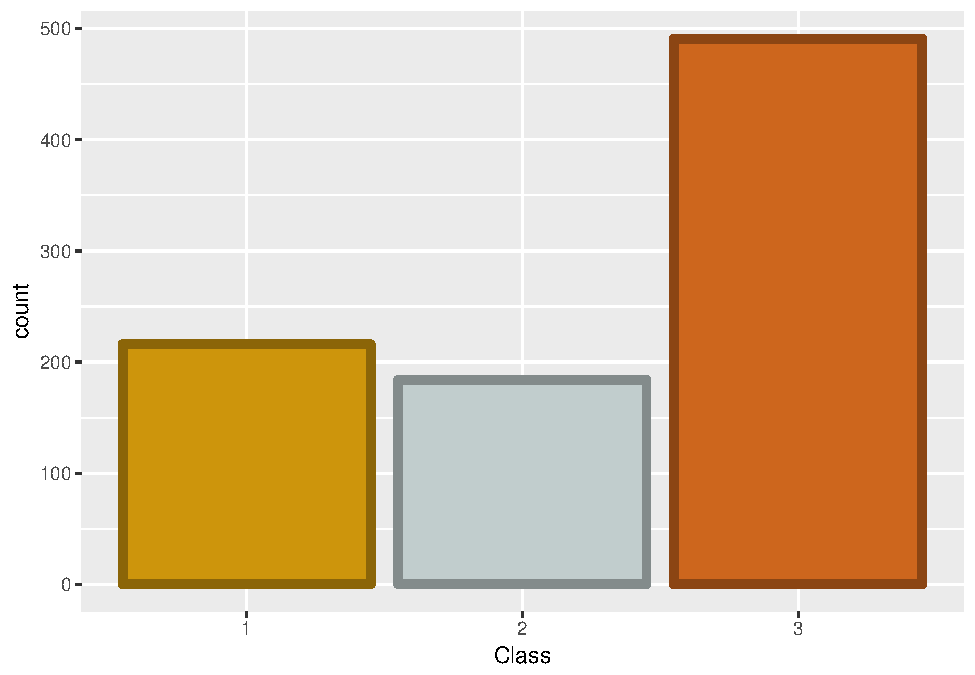
\includegraphics{titanicDataClean_files/figure-latex/set_library_plot2-1.pdf}
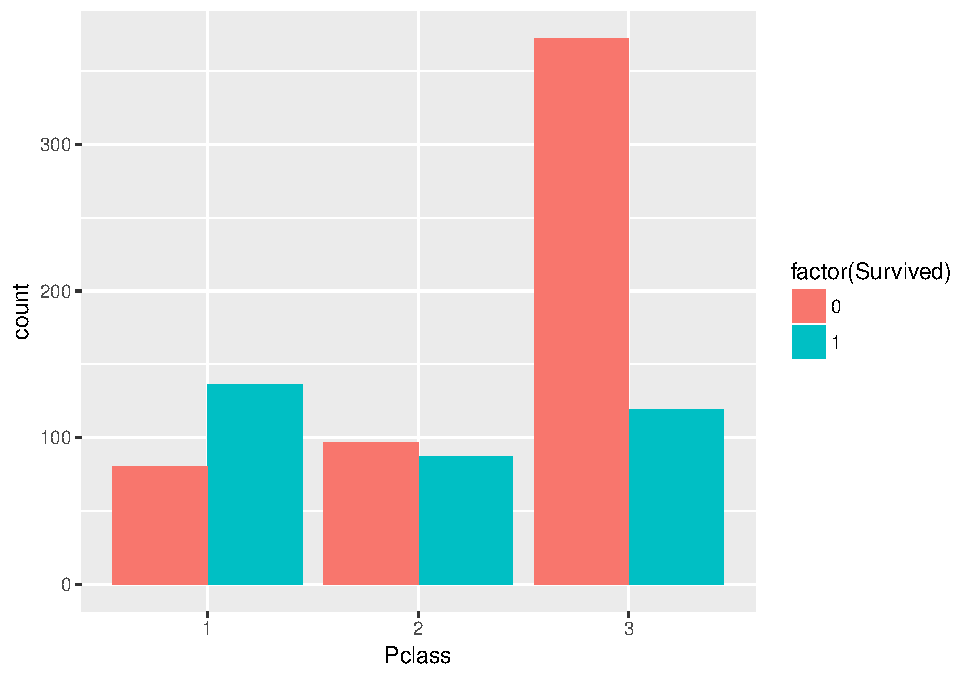
\includegraphics{titanicDataClean_files/figure-latex/set_library_plot2-2.pdf}

\subsubsection{Name}\label{name}

La longitud promedio de un nombre es de 27 caracteres con un máximo de
82.

\begin{Shaded}
\begin{Highlighting}[]
\CommentTok{# Resumen de las longitudes del nombre}
\KeywordTok{summary}\NormalTok{(}\KeywordTok{sapply}\NormalTok{(}\KeywordTok{as.character}\NormalTok{(}\KeywordTok{unique}\NormalTok{(titanic_train}\OperatorTok{$}\NormalTok{Name)),nchar))}
\end{Highlighting}
\end{Shaded}

\begin{verbatim}
##    Min. 1st Qu.  Median    Mean 3rd Qu.    Max. 
##   12,00   20,00   25,00   26,97   30,00   82,00
\end{verbatim}

\subsubsection{Sex}\label{sex}

Casi el doble de hombres:

\begin{Shaded}
\begin{Highlighting}[]
\CommentTok{#Casi el doble de hombres}
\KeywordTok{summary}\NormalTok{(titanic_train}\OperatorTok{$}\NormalTok{Sex)}
\end{Highlighting}
\end{Shaded}

\begin{verbatim}
## female   male 
##    314    577
\end{verbatim}

\begin{Shaded}
\begin{Highlighting}[]
\NormalTok{sb <-}\StringTok{ }\KeywordTok{ggplot}\NormalTok{(titanic_train, }\KeywordTok{aes}\NormalTok{(}\DataTypeTok{x=}\NormalTok{Sex)) }\OperatorTok{+}\StringTok{ }
\StringTok{  }\KeywordTok{geom_bar}\NormalTok{(}\DataTypeTok{fill=}\KeywordTok{c}\NormalTok{(}\KeywordTok{colors}\NormalTok{()[}\DecValTok{542}\NormalTok{], }\KeywordTok{colors}\NormalTok{()[}\DecValTok{121}\NormalTok{]), }
           \DataTypeTok{col=}\KeywordTok{c}\NormalTok{(}\KeywordTok{colors}\NormalTok{()[}\DecValTok{543}\NormalTok{], }\KeywordTok{colors}\NormalTok{()[}\DecValTok{123}\NormalTok{]), }\DataTypeTok{lwd =} \DecValTok{2}\NormalTok{) }\OperatorTok{+}\StringTok{ }
\StringTok{  }\KeywordTok{labs}\NormalTok{(}\DataTypeTok{x=}\StringTok{"Class"}\NormalTok{)}
\NormalTok{sb}
\end{Highlighting}
\end{Shaded}

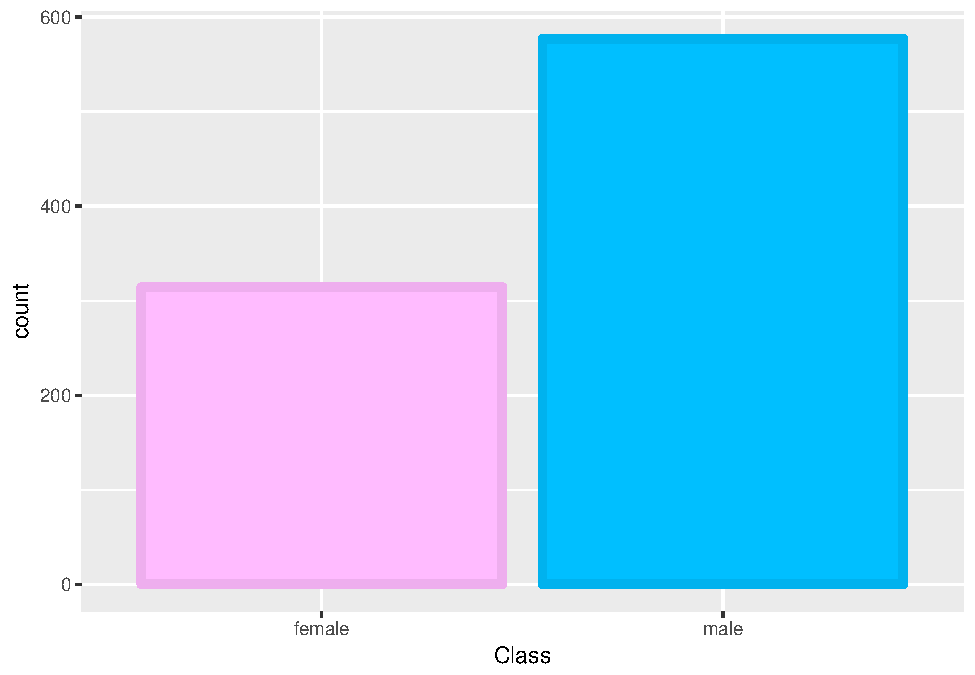
\includegraphics{titanicDataClean_files/figure-latex/var_sex-1.pdf}

\subsubsection{Age}\label{age}

Promedio de edad alrededor de los 30 años con 177 NA. Existe una
necesidad de encontrar una forma de imputar estos valores.

\begin{Shaded}
\begin{Highlighting}[]
\CommentTok{# # 177 NA's, la edad media es 28 años aka nacido en 1884 (inicio de la entrada)}
\KeywordTok{summary}\NormalTok{(titanic_train}\OperatorTok{$}\NormalTok{Age)}
\end{Highlighting}
\end{Shaded}

\begin{verbatim}
##    Min. 1st Qu.  Median    Mean 3rd Qu.    Max.    NA's 
##    0,42   20,12   28,00   29,70   38,00   80,00     177
\end{verbatim}

\begin{Shaded}
\begin{Highlighting}[]
\NormalTok{ap <-}\StringTok{ }\KeywordTok{ggplot}\NormalTok{(titanic_train, }\KeywordTok{aes}\NormalTok{(}\DataTypeTok{x=}\NormalTok{Age))}\OperatorTok{+}\KeywordTok{geom_density}\NormalTok{(}\DataTypeTok{adjust=}\NormalTok{.}\DecValTok{5}\NormalTok{)}
\NormalTok{ap}
\end{Highlighting}
\end{Shaded}

\begin{verbatim}
## Warning: Removed 177 rows containing non-finite values (stat_density).
\end{verbatim}

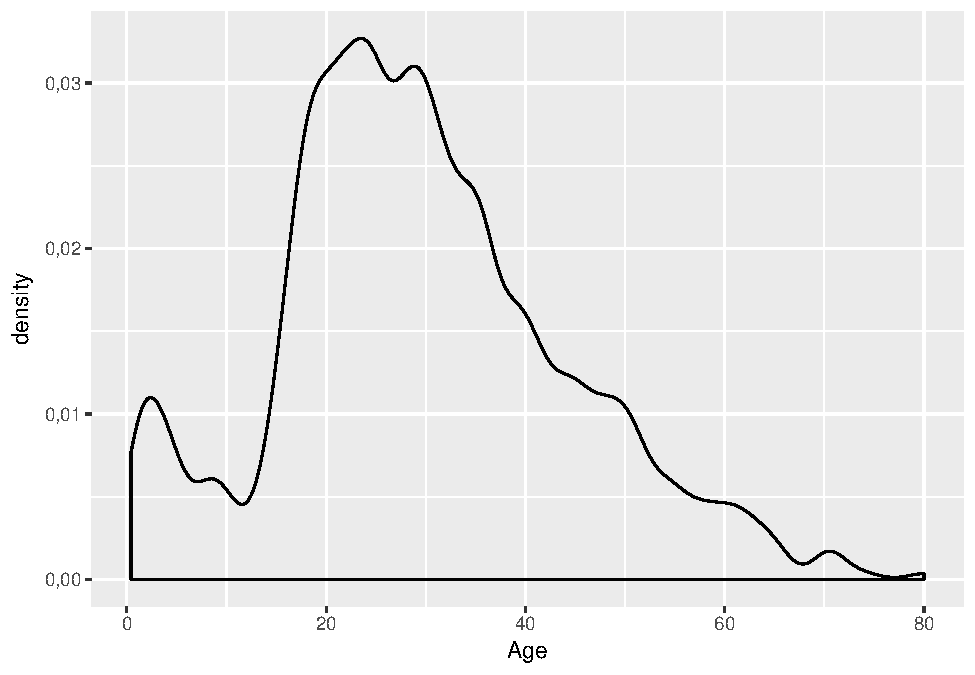
\includegraphics{titanicDataClean_files/figure-latex/var_age-1.pdf}

\subsubsection{Hermanos y cónyuges}\label{hermanos-y-conyuges}

La mayoría de las personas viajan solas. La mediana es 0, y solo
aproximadamente 1/4 de las personas están con hermanos o cónyuges.

\begin{Shaded}
\begin{Highlighting}[]
\KeywordTok{unique}\NormalTok{(titanic_train}\OperatorTok{$}\NormalTok{SibSp)}
\end{Highlighting}
\end{Shaded}

\begin{verbatim}
## [1] 1 0 3 4 2 5 8
\end{verbatim}

\begin{Shaded}
\begin{Highlighting}[]
\CommentTok{# Max Spouse es 1, crea datos de hermanos}
\CommentTok{# Max parents is 2, create children data}
\CommentTok{# Recopilar datos de riqueza de los puntos de embarque}
\NormalTok{titanic_train}\OperatorTok{$}\NormalTok{SibSp <-}\StringTok{ }\KeywordTok{as.integer}\NormalTok{(titanic_train}\OperatorTok{$}\NormalTok{SibSp) }\CommentTok{#posiblemente solo frente a variable familiar}
\KeywordTok{summary}\NormalTok{(titanic_train}\OperatorTok{$}\NormalTok{SibSp) }\CommentTok{#mediana es 0}
\end{Highlighting}
\end{Shaded}

\begin{verbatim}
##    Min. 1st Qu.  Median    Mean 3rd Qu.    Max. 
##   0,000   0,000   0,000   0,523   1,000   8,000
\end{verbatim}

\begin{Shaded}
\begin{Highlighting}[]
\KeywordTok{dim}\NormalTok{(titanic_train[titanic_train}\OperatorTok{$}\NormalTok{SibSp }\OperatorTok{>}\StringTok{ }\DecValTok{0}\NormalTok{,])}
\end{Highlighting}
\end{Shaded}

\begin{verbatim}
## [1] 283  11
\end{verbatim}

\begin{Shaded}
\begin{Highlighting}[]
\KeywordTok{dim}\NormalTok{(titanic_train[titanic_train}\OperatorTok{$}\NormalTok{SibSp }\OperatorTok{==}\StringTok{ }\DecValTok{0}\NormalTok{,])}
\end{Highlighting}
\end{Shaded}

\begin{verbatim}
## [1] 608  11
\end{verbatim}

\begin{Shaded}
\begin{Highlighting}[]
\KeywordTok{ggplot}\NormalTok{(titanic_train, }\KeywordTok{aes}\NormalTok{(}\DataTypeTok{x =}\NormalTok{ SibSp, }\DataTypeTok{fill =} \KeywordTok{factor}\NormalTok{(Survived))) }\OperatorTok{+}
\StringTok{  }\KeywordTok{geom_bar}\NormalTok{(}\DataTypeTok{stat=}\StringTok{'count'}\NormalTok{, }\DataTypeTok{position=}\StringTok{'dodge'}\NormalTok{) }\OperatorTok{+}
\StringTok{  }\KeywordTok{scale_x_continuous}\NormalTok{(}\DataTypeTok{breaks=}\KeywordTok{c}\NormalTok{(}\DecValTok{1}\OperatorTok{:}\DecValTok{7}\NormalTok{)) }\OperatorTok{+}
\StringTok{  }\KeywordTok{labs}\NormalTok{(}\DataTypeTok{x =} \StringTok{'SibSp'}\NormalTok{)}
\end{Highlighting}
\end{Shaded}

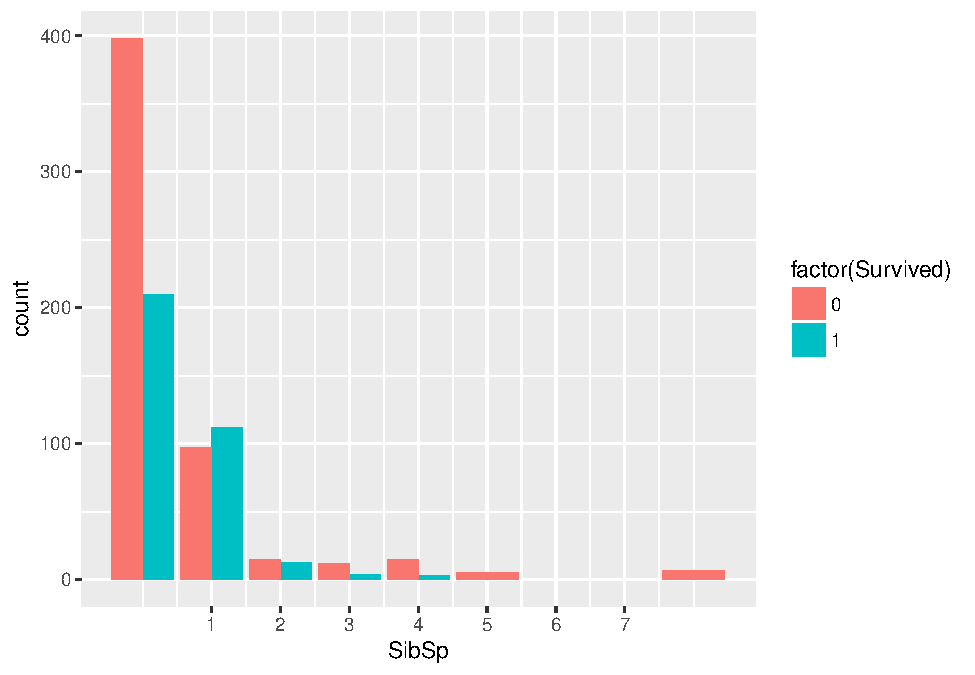
\includegraphics{titanicDataClean_files/figure-latex/var_spouses-1.pdf}

Estas tablas sugieren que la única configuración beneficiosa es tener 1
hermano o cónyuge. Ellos son el único grupo que tiene más probabilidades
de sobrevivir. Esto podría ser indicativo de madres solteras, o tal vez
de parejas, aunque Jack y Rose son un contador formidable de esa
proposición.

\begin{verbatim}
## Warning: Removed 2 rows containing missing values (geom_bar).
\end{verbatim}

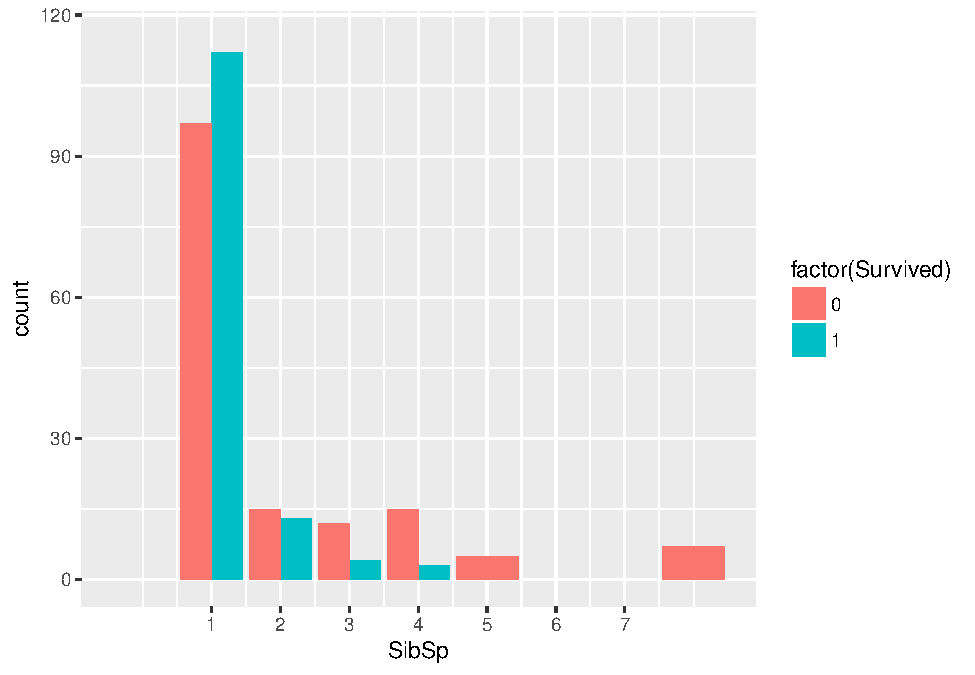
\includegraphics{titanicDataClean_files/figure-latex/unnamed-chunk-3-1.pdf}

\subsubsection{Padres e hijos}\label{padres-e-hijos}

Esto también sugiere que la mayoría de la gente no tiene familia.
Aproximadamente 1/4 tienen padres o niños a bordo.

\begin{Shaded}
\begin{Highlighting}[]
\KeywordTok{unique}\NormalTok{(titanic_train}\OperatorTok{$}\NormalTok{Parch) }
\end{Highlighting}
\end{Shaded}

\begin{verbatim}
## [1] 0 1 2 5 3 4 6
\end{verbatim}

\begin{Shaded}
\begin{Highlighting}[]
\KeywordTok{summary}\NormalTok{(titanic_train}\OperatorTok{$}\NormalTok{Parch) }
\end{Highlighting}
\end{Shaded}

\begin{verbatim}
##    Min. 1st Qu.  Median    Mean 3rd Qu.    Max. 
##  0,0000  0,0000  0,0000  0,3816  0,0000  6,0000
\end{verbatim}

Hay 213 personas que viajan con sus hijos o padres.

\begin{Shaded}
\begin{Highlighting}[]
\KeywordTok{dim}\NormalTok{(titanic_train[titanic_train}\OperatorTok{$}\NormalTok{Parch }\OperatorTok{>}\StringTok{ }\DecValTok{0}\NormalTok{,]) }
\end{Highlighting}
\end{Shaded}

\begin{verbatim}
## [1] 213  11
\end{verbatim}

Los otros 678 están solos.

\begin{Shaded}
\begin{Highlighting}[]
\KeywordTok{dim}\NormalTok{(titanic_train[titanic_train}\OperatorTok{$}\NormalTok{Parch }\OperatorTok{==}\StringTok{ }\DecValTok{0}\NormalTok{,])}
\end{Highlighting}
\end{Shaded}

\begin{verbatim}
## [1] 678  11
\end{verbatim}

Este primer cuadro muestra la abrumadora desventaja de viajar solo.

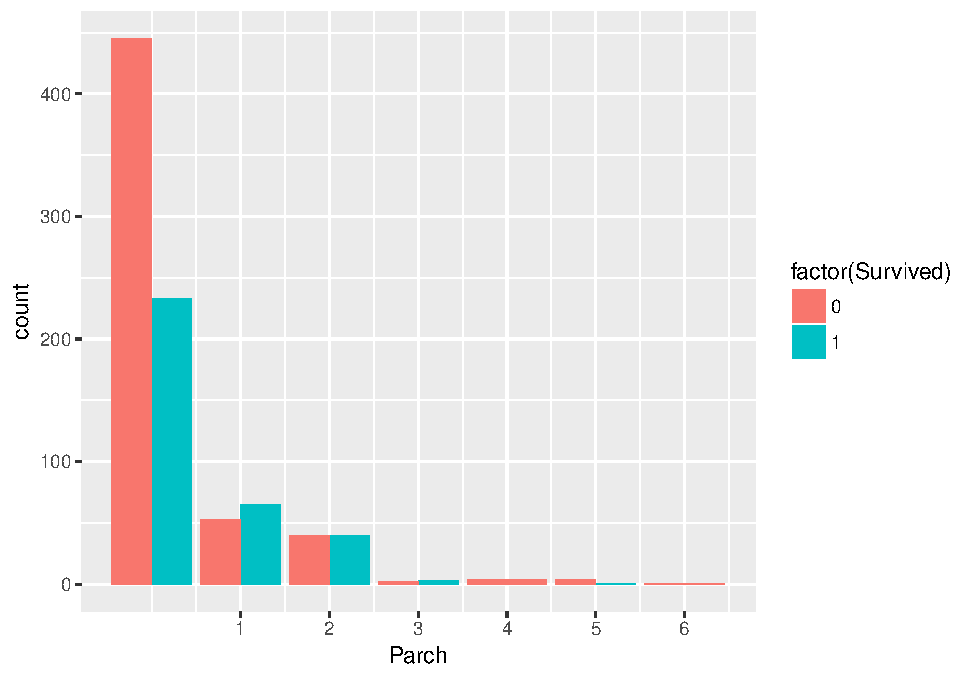
\includegraphics{titanicDataClean_files/figure-latex/unnamed-chunk-4-1.pdf}

Este muestra que tener una relación 1-3 niños/padres es potencialmente
beneficioso.

\begin{verbatim}
## Warning: Removed 2 rows containing missing values (geom_bar).
\end{verbatim}

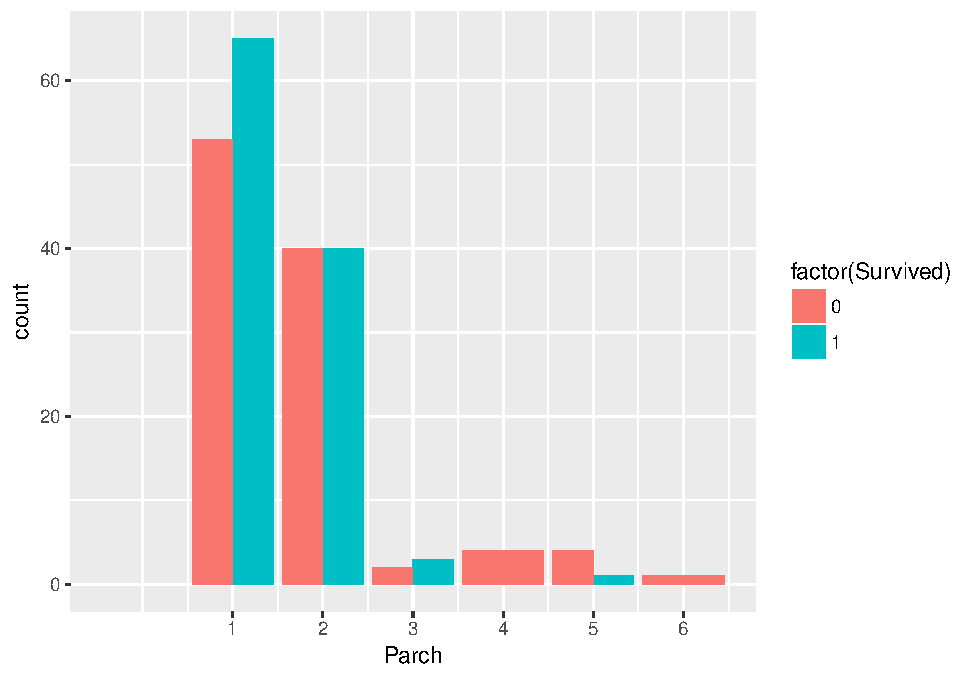
\includegraphics{titanicDataClean_files/figure-latex/unnamed-chunk-5-1.pdf}

\subsubsection{Ticket}\label{ticket}

Hay 681 identificadores de tickets únicos. Los boletos tienen
identificadores de prefijo y dígitos iniciales limitados que podrían
codificar más información sobre el pasajero.

\begin{verbatim}
## [1] 681
\end{verbatim}

Este gráfico muestra que algunos de los prefijos de tickt están
asociados con precios más altos. La tarifa ya debería dar cuenta de esta
variación, por lo tanto, a menos que podamos encontrar otra relación con
el prefijo, entonces no vale la pena incluir esta variable.

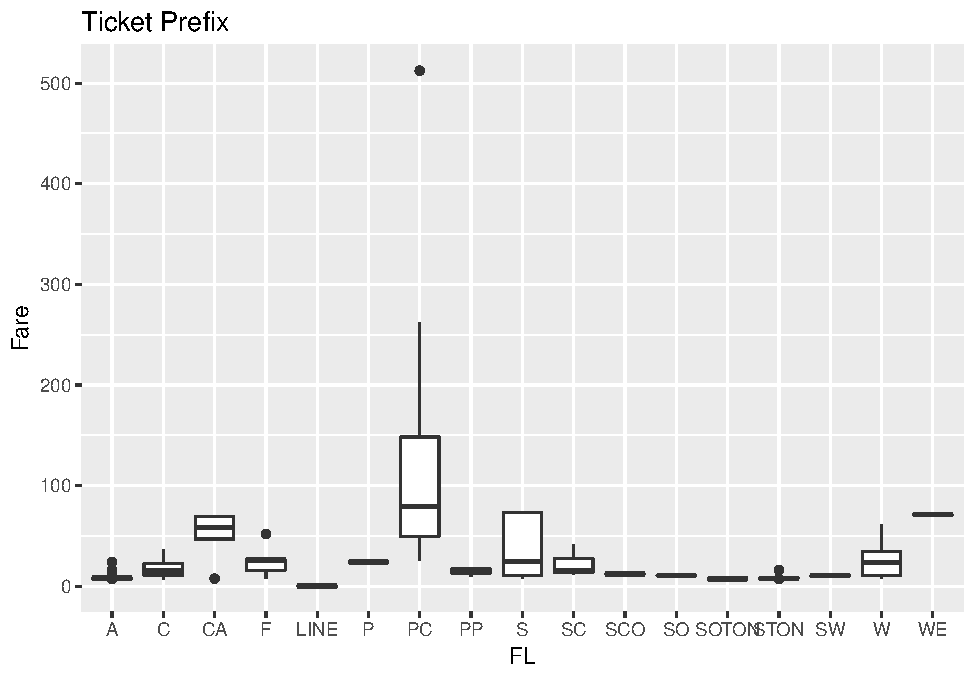
\includegraphics{titanicDataClean_files/figure-latex/plot-1.pdf}

Esto confirma que el ticket codifica más información, pero para que sea
útil tendrá que cavar más profundo. La gráfica a continuación muestra
que aquellos con el prefijo de ticket para PC tienen muchas más
probabilidades de sobrevivir. Este gráfico está confundido por el precio
del boleto. Algunos de los prefijos son intrigantes. A, CA, SOTON y W
tienen tasas de bajas extremadamente altas en relación con todas las
demás.

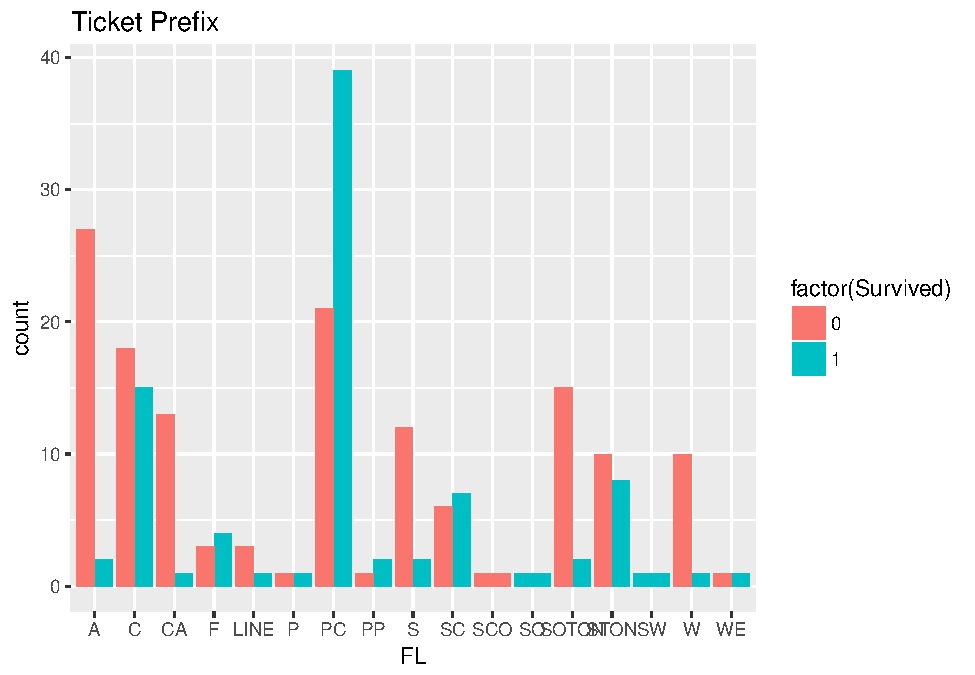
\includegraphics{titanicDataClean_files/figure-latex/ticketplot-1.pdf}

Si profundizamos un poco más, ¿qué tienen en común estos prefijos? Si
miramos la longitud de los componentes numéricos de los tickets,
encontramos algo interesante: Los sufijos que mencionamos generalmente
tienen números de ticket más cortos. El máximo es 2 menos, y la mediana
es 2 menos. Esto es particularmente interesante porque hay entradas sin
prefijos que también tienen entradas más cortas, así que tal vez
tengamos algo bueno.

\begin{Shaded}
\begin{Highlighting}[]
\NormalTok{tfix <-}\StringTok{ }\NormalTok{tpref[tpref}\OperatorTok{$}\NormalTok{FL }\OperatorTok\StringTok{ }\KeywordTok{c}\NormalTok{(}\StringTok{"A"}\NormalTok{, }\StringTok{"CA"}\NormalTok{, }\StringTok{"Soton"}\NormalTok{, }\StringTok{"W"}\NormalTok{),]}
\KeywordTok{summary}\NormalTok{(}\KeywordTok{sapply}\NormalTok{(}\KeywordTok{as.character}\NormalTok{(titanic_train}\OperatorTok{$}\NormalTok{FT),nchar))}
\end{Highlighting}
\end{Shaded}

\begin{verbatim}
##    Min. 1st Qu.  Median    Mean 3rd Qu.    Max.    NA's 
##   3,000   5,000   6,000   5,375   6,000   7,000       6
\end{verbatim}

\begin{Shaded}
\begin{Highlighting}[]
\KeywordTok{summary}\NormalTok{(}\KeywordTok{sapply}\NormalTok{(}\KeywordTok{as.character}\NormalTok{(tfix}\OperatorTok{$}\NormalTok{FT), nchar))}
\end{Highlighting}
\end{Shaded}

\begin{verbatim}
##    Min. 1st Qu.  Median    Mean 3rd Qu.    Max. 
##   3,000   4,000   4,000   4,315   5,000   5,000
\end{verbatim}

Regresaremos sobre esto más tarde una vez que completemos esta
decodificación.

\begin{Shaded}
\begin{Highlighting}[]
\NormalTok{titanic_train}\OperatorTok{$}\NormalTok{ticketlength <-}\StringTok{ }\KeywordTok{sapply}\NormalTok{(}\KeywordTok{as.character}\NormalTok{(titanic_train}\OperatorTok{$}\NormalTok{FT),nchar)}
\end{Highlighting}
\end{Shaded}

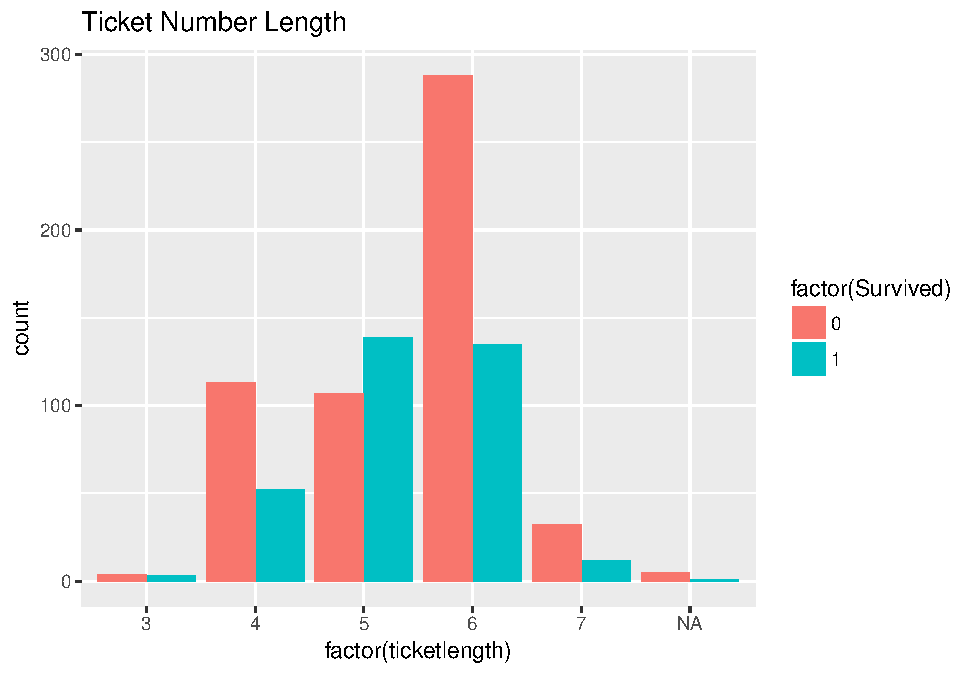
\includegraphics{titanicDataClean_files/figure-latex/plot23-1.pdf}
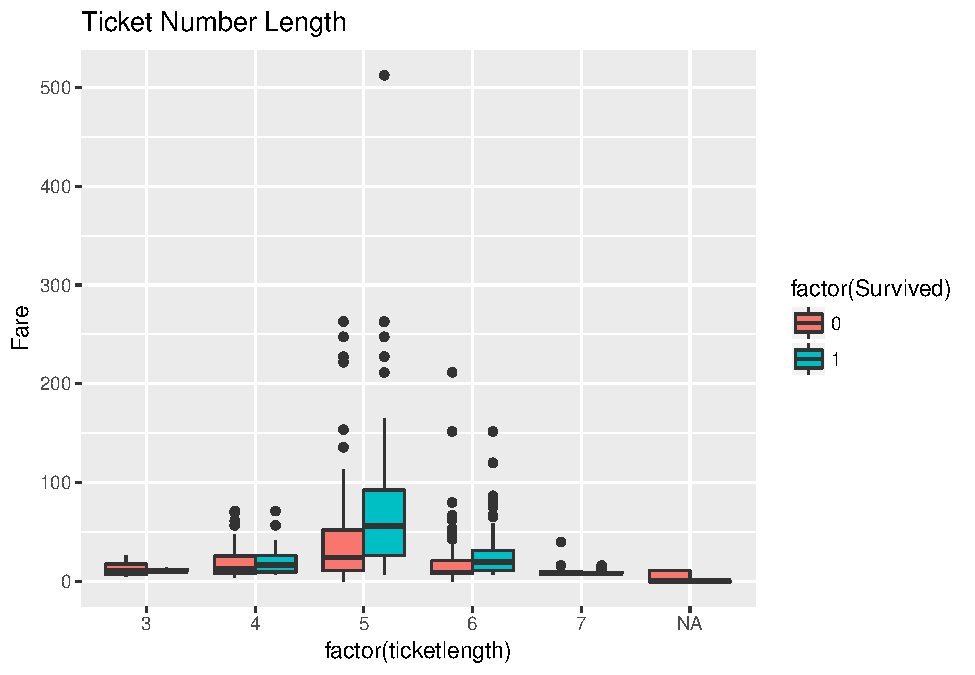
\includegraphics{titanicDataClean_files/figure-latex/plot23-2.pdf}

A riesgo de ir un paso demasiado lejos, veamos los números de los
boletos individuales. La premisa es que no son aleatorios y
potencialmente codifican datos de ubicación de pasajeros que podrían
afectar el resultado de la supervivencia. El desglose de los precios se
incluye junto para verificar el efecto de confusión.

Desde mi punto de vista, parece que hay efectos interesantes sucediendo
en los primeros 5 dígitos. La gran noticia es que no tenemos que
entenderlo completamente: ahí es donde entra el aprendizaje automático.

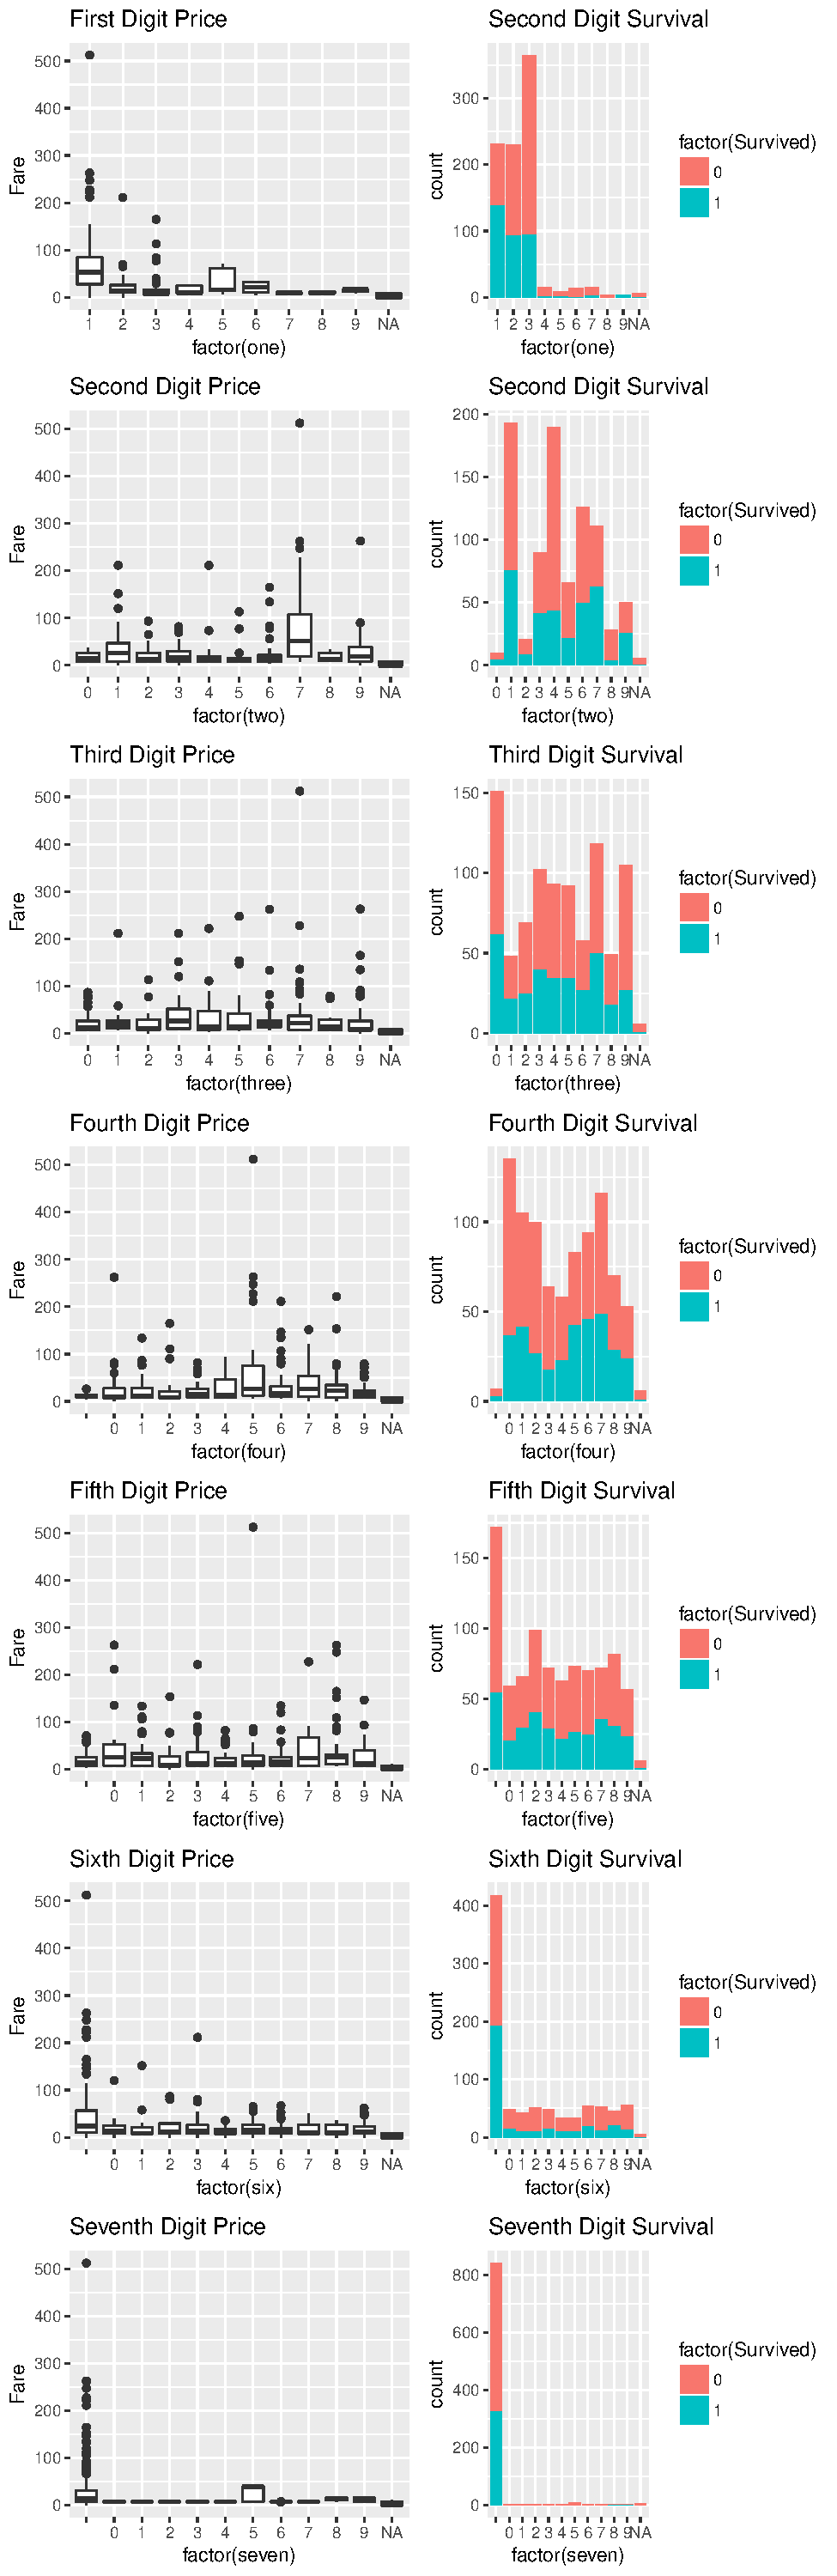
\includegraphics{titanicDataClean_files/figure-latex/plot2-1.pdf}

\subsubsection{Fare}\label{fare}

Aparentemente en el Titanic, solo los hombres obtienen viajes gratis.
Las mujeres pagan entre 5 y 24 dolares más por boleto, dependiendo de la
clase.

\begin{Shaded}
\begin{Highlighting}[]
\NormalTok{titanic_train[titanic_train}\OperatorTok{$}\NormalTok{Fare}\OperatorTok{==}\DecValTok{0}\NormalTok{,]}\OperatorTok{$}\NormalTok{Sex}
\end{Highlighting}
\end{Shaded}

\begin{verbatim}
##  [1] male male male male male male male male male male male male male male
## [15] male
## Levels: female male
\end{verbatim}

Hay 248 precios únicos de entradas.

\begin{Shaded}
\begin{Highlighting}[]
\KeywordTok{length}\NormalTok{(}\KeywordTok{unique}\NormalTok{(titanic_train}\OperatorTok{$}\NormalTok{Fare))}
\end{Highlighting}
\end{Shaded}

\begin{verbatim}
## [1] 248
\end{verbatim}

Como se esperaba, la primera clase es mucho más costosa.

\begin{Shaded}
\begin{Highlighting}[]
\NormalTok{titanic_train }\OperatorTok\StringTok{ }\KeywordTok{group_by}\NormalTok{(Pclass) }\OperatorTok\StringTok{ }\KeywordTok{summarise_each}\NormalTok{(}\KeywordTok{funs}\NormalTok{(min, max, mean, median),Fare) }
\end{Highlighting}
\end{Shaded}

\begin{verbatim}
## # A tibble: 3 x 5
##   Pclass Fare_min Fare_max Fare_mean Fare_median
##   <fctr>    <dbl>    <dbl>     <dbl>       <dbl>
## 1 1             0    512        84.2       60.3 
## 2 2             0     73.5      20.7       14.2 
## 3 3             0     69.6      13.7        8.05
\end{verbatim}

Resulta que las mujeres pagan 24 dolares más en promedio por boleto.

\begin{Shaded}
\begin{Highlighting}[]
\NormalTok{titanic_train }\OperatorTok\StringTok{ }\KeywordTok{group_by}\NormalTok{(Sex) }\OperatorTok\StringTok{ }\KeywordTok{summarise_each}\NormalTok{(}\KeywordTok{funs}\NormalTok{(min, max, mean, median),Fare)}
\end{Highlighting}
\end{Shaded}

\begin{verbatim}
## # A tibble: 2 x 5
##   Sex    Fare_min Fare_max Fare_mean Fare_median
##   <fctr>    <dbl>    <dbl>     <dbl>       <dbl>
## 1 female     6.75      512      44.5        23.0
## 2 male       0         512      25.5        10.5
\end{verbatim}

\subsubsection{Cabin}\label{cabin}

Hay 163 valores de cabina declarados con 148 únicos, faltan muchos. Es
posible que la información de la cabina se pueda imputar según el número
de boleto, el puerto de embarque y la clase.

\begin{Shaded}
\begin{Highlighting}[]
\KeywordTok{length}\NormalTok{(}\KeywordTok{unique}\NormalTok{(titanic_train}\OperatorTok{$}\NormalTok{Cabin))}
\end{Highlighting}
\end{Shaded}

\begin{verbatim}
## [1] 148
\end{verbatim}

\begin{verbatim}
## [1] 204
\end{verbatim}

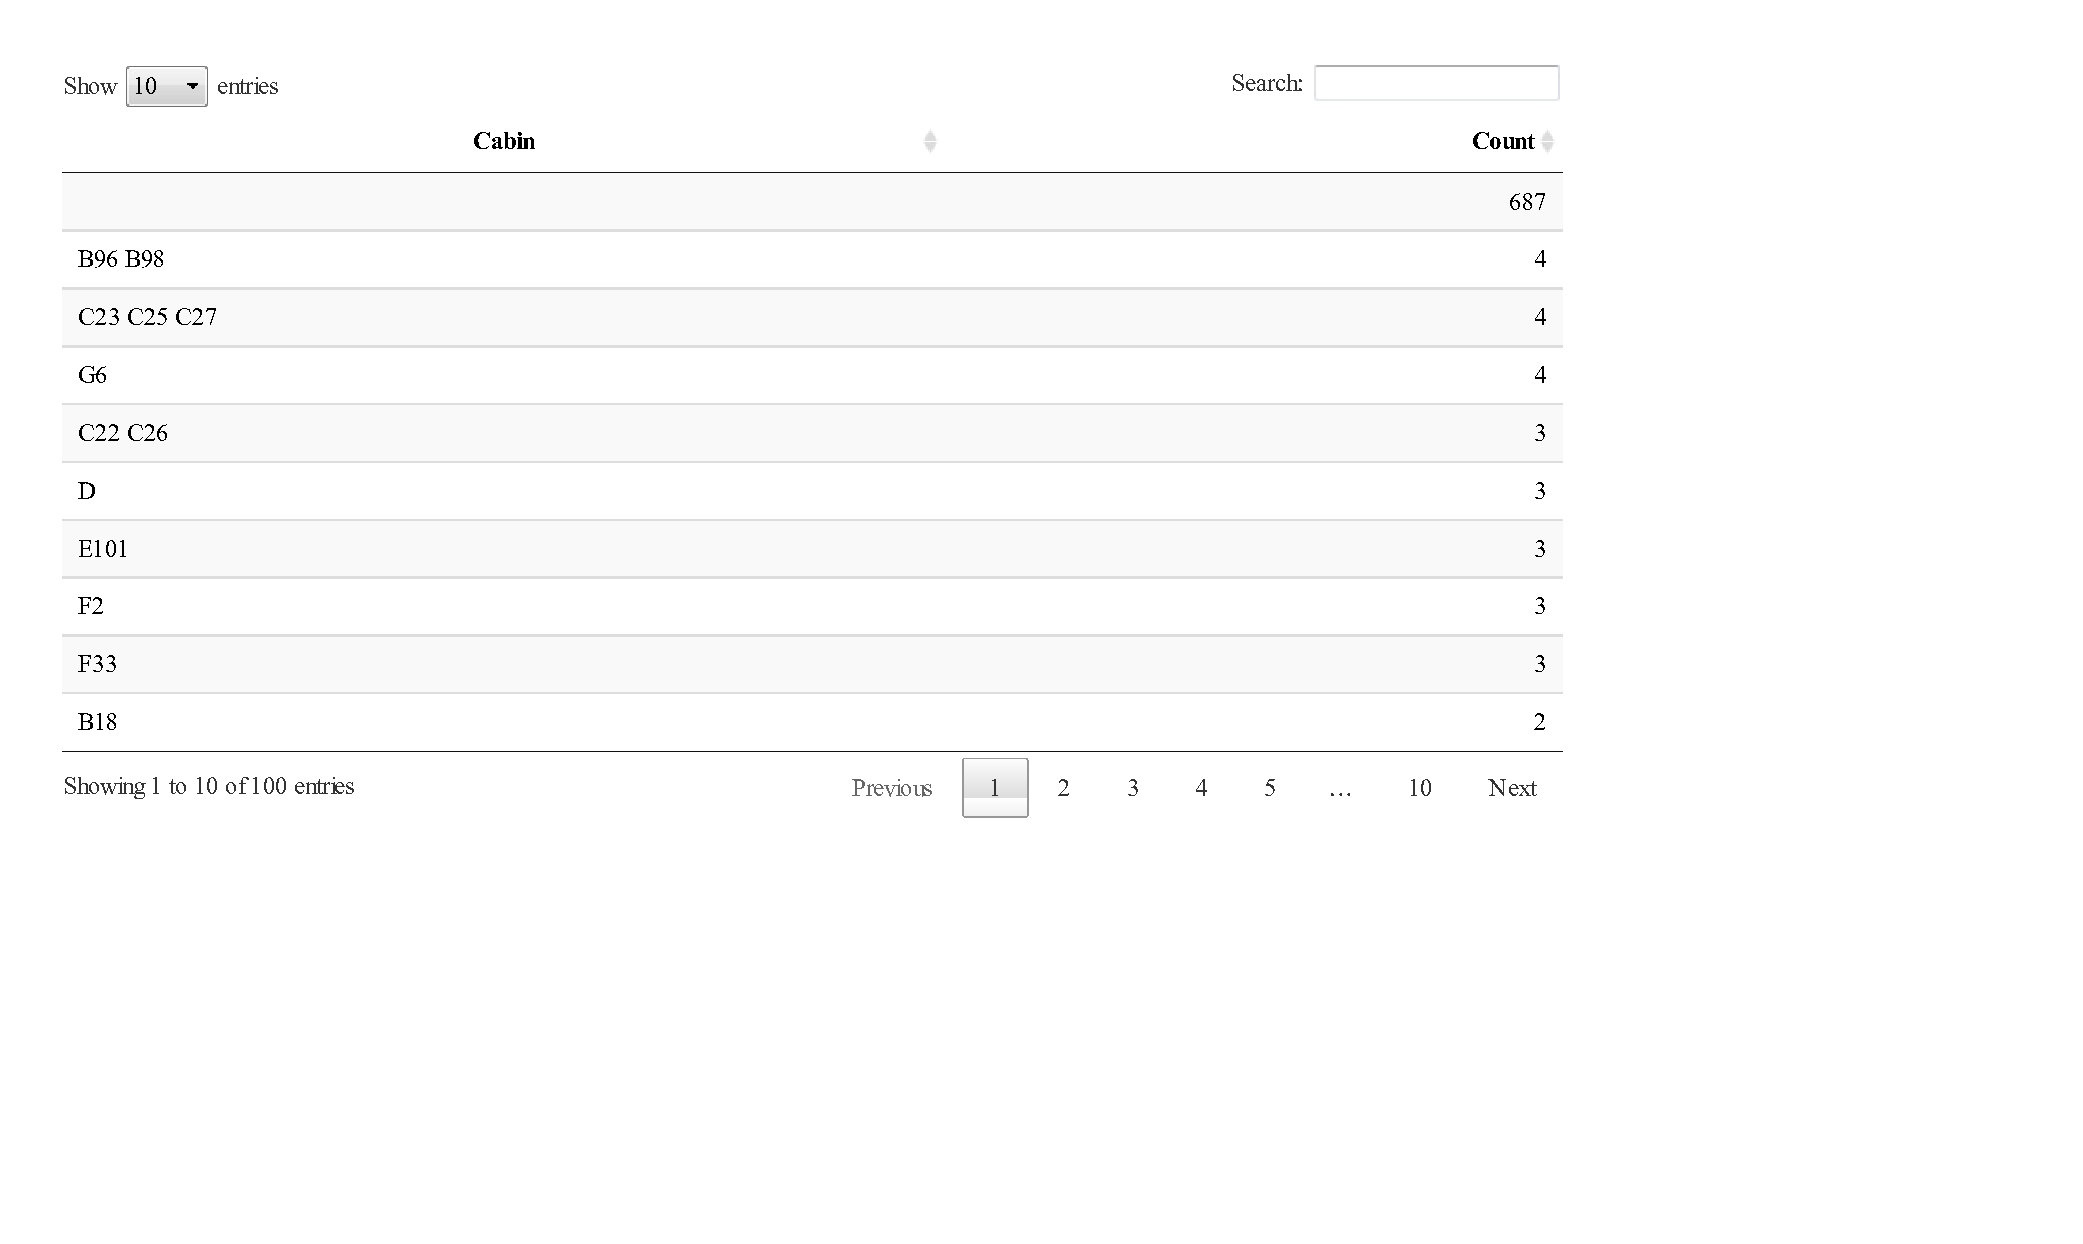
\includegraphics{titanicDataClean_files/figure-latex/cabin-1.pdf}

Creamos ahora una variable de la letra de Cabin.

\begin{Shaded}
\begin{Highlighting}[]
\NormalTok{titanic_train}\OperatorTok{$}\NormalTok{CL <-}\StringTok{ }\KeywordTok{substring}\NormalTok{(titanic_train}\OperatorTok{$}\NormalTok{Cabin, }\DecValTok{1}\NormalTok{, }\DecValTok{1}\NormalTok{)}
\NormalTok{titanic_train}\OperatorTok{$}\NormalTok{CL <-}\StringTok{ }\KeywordTok{as.factor}\NormalTok{(titanic_train}\OperatorTok{$}\NormalTok{CL)}
\KeywordTok{unique}\NormalTok{(titanic_train}\OperatorTok{$}\NormalTok{CL)}
\end{Highlighting}
\end{Shaded}

\begin{verbatim}
## [1]   C E G D A B F T
## Levels:  A B C D E F G T
\end{verbatim}

El subconjunto es desproporcionado para la primera clase en Cherbourg y
Southampton.

\begin{Shaded}
\begin{Highlighting}[]
\KeywordTok{summary}\NormalTok{(titanic_train[}\OperatorTok{!}\KeywordTok{substring}\NormalTok{(titanic_train}\OperatorTok{$}\NormalTok{Cabin, }\DecValTok{1}\NormalTok{, }\DecValTok{1}\NormalTok{) }\OperatorTok{==}\StringTok{ ""}\NormalTok{,]}\OperatorTok{$}\NormalTok{Embarked)}
\end{Highlighting}
\end{Shaded}

\begin{verbatim}
##       C   Q   S 
##   2  69   4 129
\end{verbatim}

\begin{Shaded}
\begin{Highlighting}[]
\KeywordTok{summary}\NormalTok{(titanic_train[}\OperatorTok{!}\KeywordTok{substring}\NormalTok{(titanic_train}\OperatorTok{$}\NormalTok{Cabin, }\DecValTok{1}\NormalTok{, }\DecValTok{1}\NormalTok{) }\OperatorTok{==}\StringTok{ ""}\NormalTok{,]}\OperatorTok{$}\NormalTok{Pclass)}
\end{Highlighting}
\end{Shaded}

\begin{verbatim}
##   1   2   3 
## 176  16  12
\end{verbatim}

El primer gráfico muestra que las cabinas B y C son más caras.

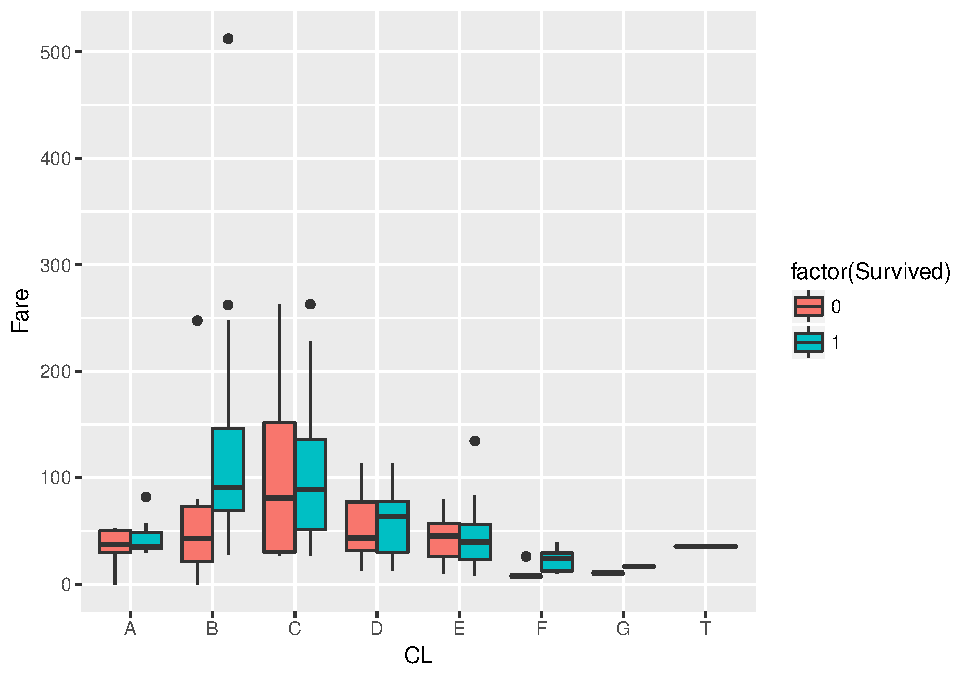
\includegraphics{titanicDataClean_files/figure-latex/cabinsplit-1.pdf}

El segundo gráfico muestra que puede haber algunas relaciones
interesantes aquí para la supervivencia. Es importante recordar que este
subconjunto ya es más probable que sobreviva debido a su estado de
primera clase.

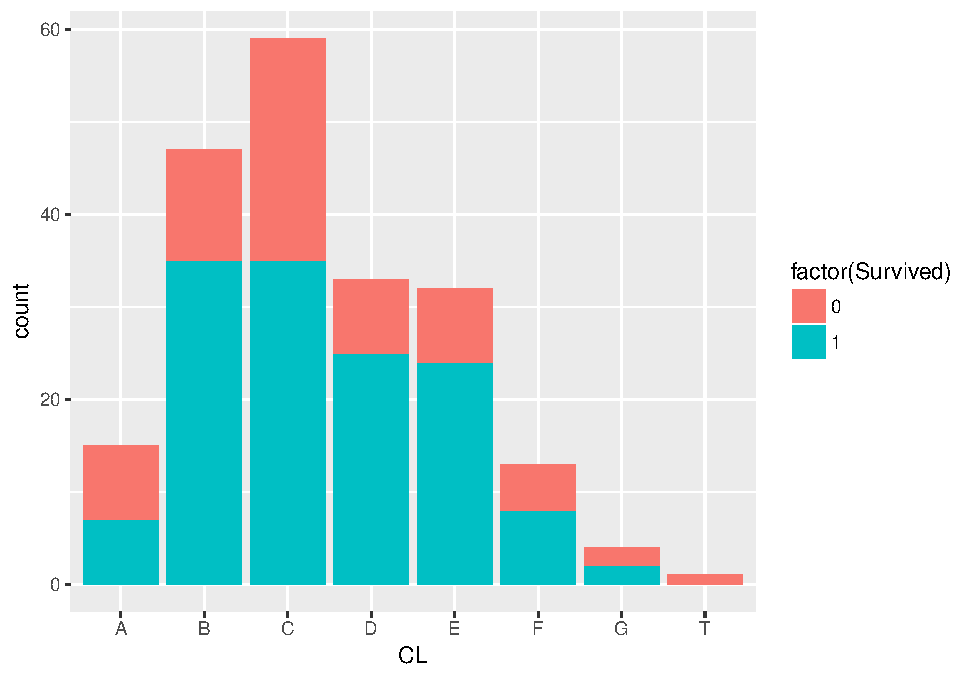
\includegraphics{titanicDataClean_files/figure-latex/cabinsplit2-1.pdf}

Según los datos, parece difícil imputar con precisión las asignaciones
de cabina para el resto del conjunto de datos. En cambio, creemos un
variable binaria para ``habitación asignada'' o ``no asignada''. Esto
podría representar una mayor variación en el conjunto de datos inicial.
Una de las hipótesis es que las personas que tienen asignada una
habitación tienen alguna posición o estatus y tienen prioridad de
elección, lo que puede reflejarse en relación con su supervivencia.

\begin{Shaded}
\begin{Highlighting}[]
\NormalTok{titanic_train}\OperatorTok{$}\NormalTok{Assigned <-}\StringTok{ }\DecValTok{0}
\NormalTok{titanic_train[}\OperatorTok{!}\KeywordTok{substring}\NormalTok{(titanic_train}\OperatorTok{$}\NormalTok{Cabin, }\DecValTok{1}\NormalTok{, }\DecValTok{1}\NormalTok{) }\OperatorTok{==}\StringTok{ ""}\NormalTok{,]}\OperatorTok{$}\NormalTok{Assigned <-}\StringTok{ }\DecValTok{1}
\end{Highlighting}
\end{Shaded}

\subsubsection{Embarked}\label{embarked}

Hay 3 ubicaciones de salida, la mayoría de las personas son de
Southampton, Cherburgo y Queenstown.

\begin{Shaded}
\begin{Highlighting}[]
\KeywordTok{unique}\NormalTok{(titanic_train}\OperatorTok{$}\NormalTok{Embarked) }
\end{Highlighting}
\end{Shaded}

\begin{verbatim}
## [1] S C Q  
## Levels:  C Q S
\end{verbatim}

\begin{Shaded}
\begin{Highlighting}[]
\KeywordTok{summary}\NormalTok{(titanic_train}\OperatorTok{$}\NormalTok{Embarked)}
\end{Highlighting}
\end{Shaded}

\begin{verbatim}
##       C   Q   S 
##   2 168  77 644
\end{verbatim}

Hay 2 valores faltantes para el punto de embarque. Lo que nos lleva a la
imputación.

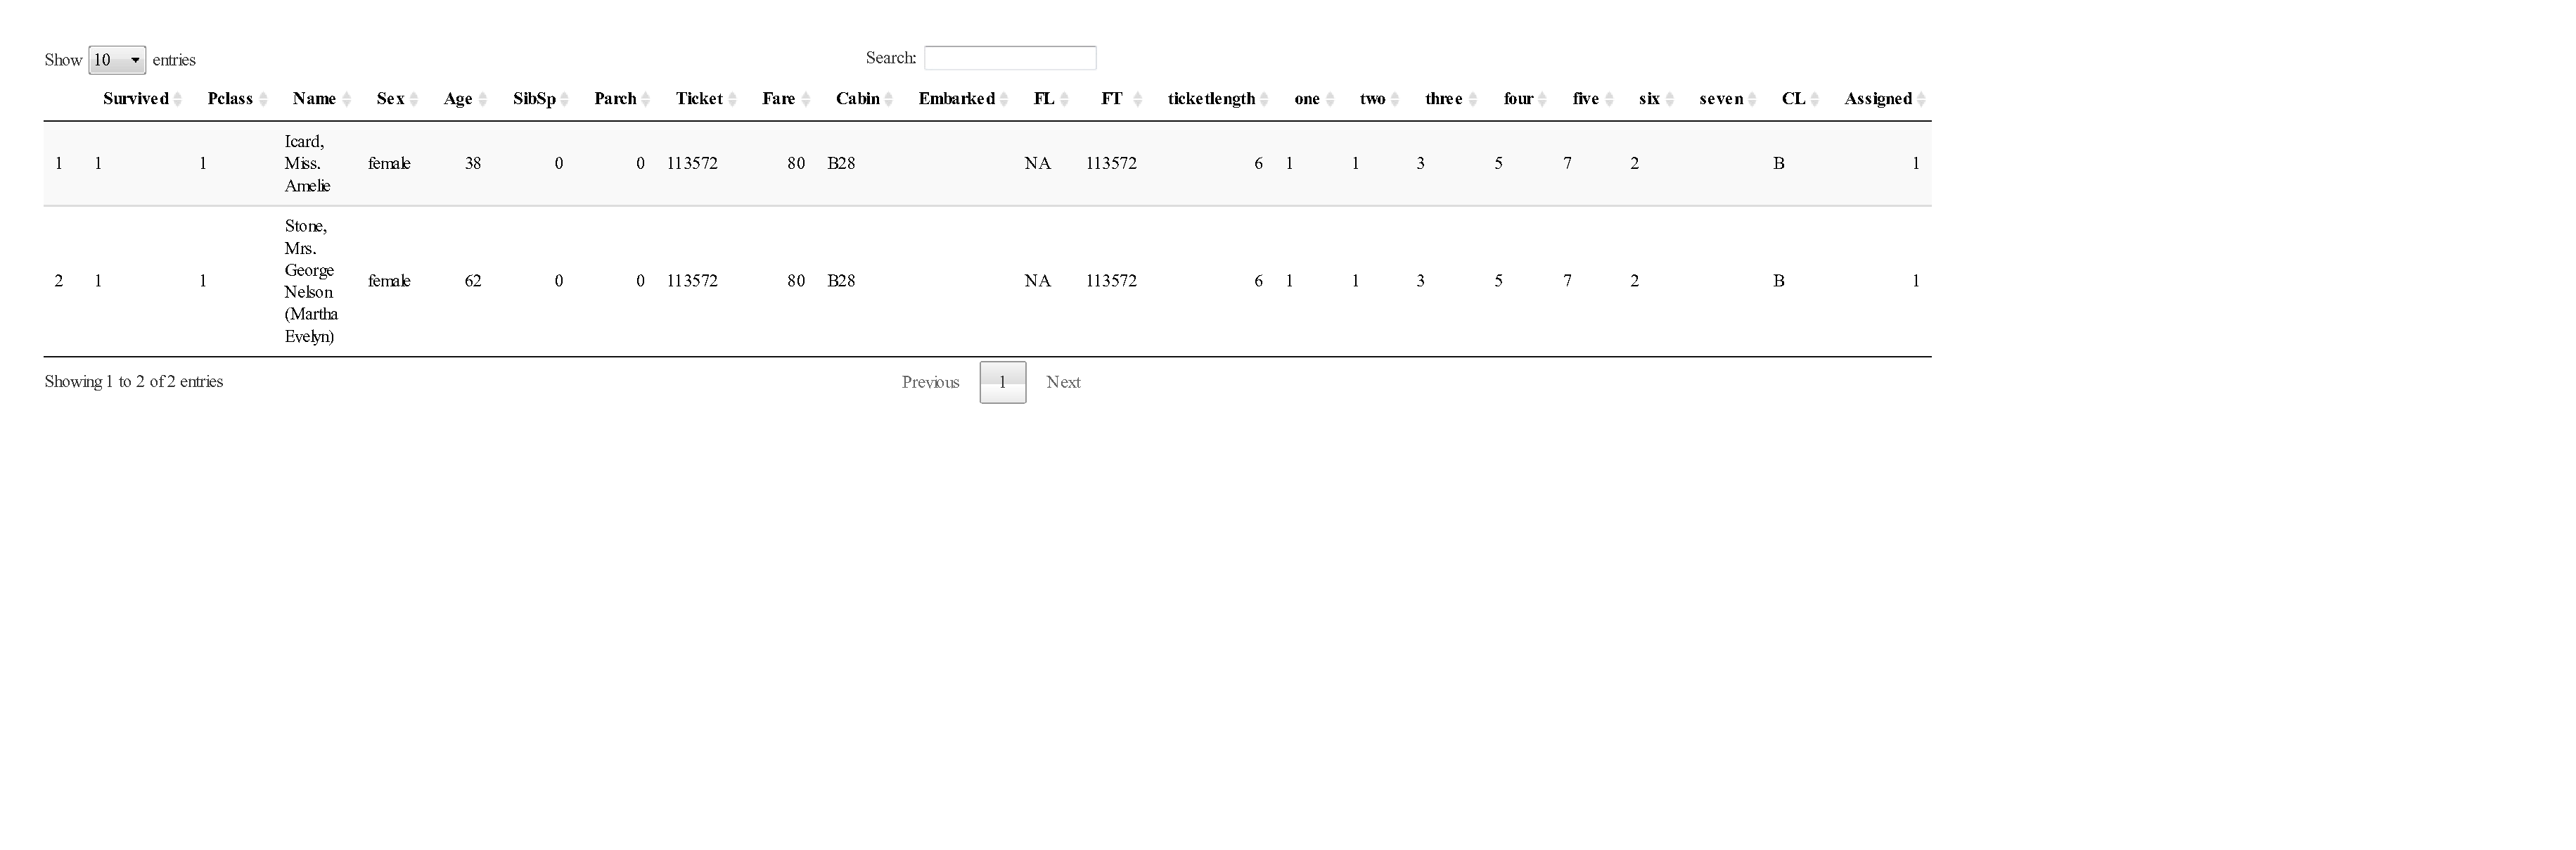
\includegraphics{titanicDataClean_files/figure-latex/miss-1.pdf}

\subsubsection{Ajuste de los datos con ceros o valores
nulos}\label{ajuste-de-los-datos-con-ceros-o-valores-nulos}

Los únicos valores faltantes se encuentran en las columnas Cabin, Age y
Embarked.

\begin{verbatim}
##     Survived       Pclass         Name          Sex          Age 
##            0            0            0            0           NA 
##        SibSp        Parch       Ticket         Fare        Cabin 
##            0            0            0            0          687 
##     Embarked           FL           FT ticketlength          one 
##            2            0           NA           NA           NA 
##          two        three         four         five          six 
##           NA           NA           NA           NA           NA 
##        seven           CL     Assigned 
##           NA          687            0
\end{verbatim}

\begin{verbatim}
##     Survived       Pclass         Name          Sex          Age 
##            0            0            0            0          177 
##        SibSp        Parch       Ticket         Fare        Cabin 
##            0            0            0            0            0 
##     Embarked           FL           FT ticketlength          one 
##            0            0            6            6            6 
##          two        three         four         five          six 
##            6            6            6            6            6 
##        seven           CL     Assigned 
##            6            0            0
\end{verbatim}

Ajustamos los datos faltantes en la variable Age:

\begin{Shaded}
\begin{Highlighting}[]
\NormalTok{titanic_train <-}\StringTok{ }\KeywordTok{as.data.frame}\NormalTok{(titanic_train)}
\CommentTok{#imputar los valores de edad faltantes con el paquete MICE}
\NormalTok{impute <-}\StringTok{ }\KeywordTok{mice}\NormalTok{(titanic_train[, }\OperatorTok{!}\KeywordTok{names}\NormalTok{(titanic_train) }\OperatorTok\StringTok{ }\KeywordTok{c}\NormalTok{(}\StringTok{'PassengerId'}\NormalTok{,}\StringTok{'Name'}\NormalTok{,}\StringTok{'Ticket'}\NormalTok{,}\StringTok{'Cabin'}\NormalTok{,}\StringTok{'Survived'}\NormalTok{, }\StringTok{'Assigned'}\NormalTok{,}\StringTok{'FL'}\NormalTok{,}\StringTok{'FT'}\NormalTok{,}\StringTok{'ticketlength'}\NormalTok{,}\StringTok{'one'}\NormalTok{,}\StringTok{'two'}\NormalTok{,}\StringTok{'three'}\NormalTok{,}\StringTok{'four'}\NormalTok{,}\StringTok{'five'}\NormalTok{,}\StringTok{'six'}\NormalTok{,}\StringTok{'seven'}\NormalTok{)], }\DataTypeTok{method=}\StringTok{'rf'}\NormalTok{)}

\NormalTok{trained_mouse <-}\StringTok{ }\KeywordTok{complete}\NormalTok{(impute)}
\end{Highlighting}
\end{Shaded}

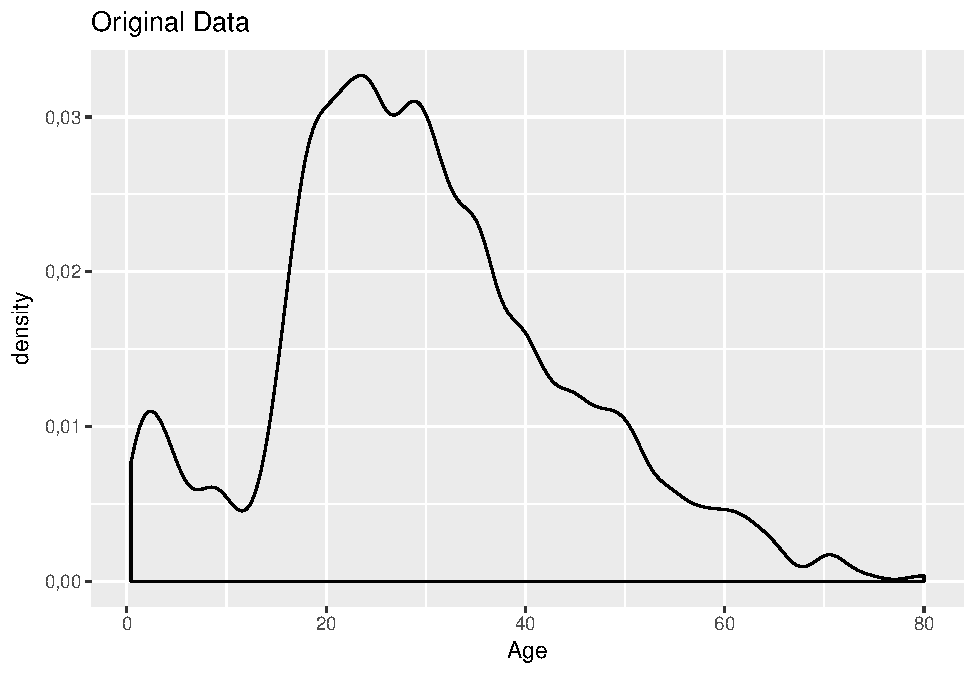
\includegraphics{titanicDataClean_files/figure-latex/pplot-1.pdf}
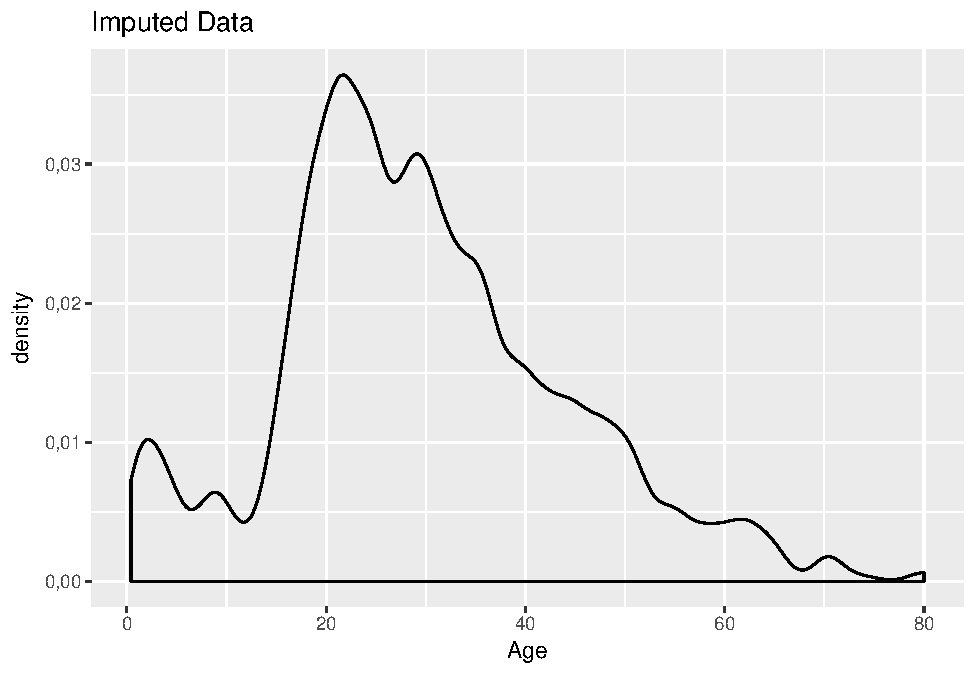
\includegraphics{titanicDataClean_files/figure-latex/pplot-2.pdf}

Dado que los resultados están razonablemente bien emparejados, podemos
reemplazar la columna original con los valores imputados.

\begin{Shaded}
\begin{Highlighting}[]
\NormalTok{titanic_train}\OperatorTok{$}\NormalTok{Age <-}\StringTok{ }\NormalTok{trained_mouse}\OperatorTok{$}\NormalTok{Age}
\end{Highlighting}
\end{Shaded}

\textbf{Ahora vamos a analizar y ajustar los valores en la variable
Enbarked.}

Ahora estamos en esos 2 valores de la variable Embarked que faltan. Lo
primero que viene a la mente es verificar con el valor de la variable
Cabin. A partir de los datos, todas las cabinas que comienzan en B se
embarcaron desde Southampton o Charbourg.

\begin{Shaded}
\begin{Highlighting}[]
\KeywordTok{unique}\NormalTok{(titanic_train[}\KeywordTok{grep}\NormalTok{(}\StringTok{"*^B"}\NormalTok{, titanic_train}\OperatorTok{$}\NormalTok{Cabin),]}\OperatorTok{$}\NormalTok{Embarked)}
\end{Highlighting}
\end{Shaded}

\begin{verbatim}
## [1] C   S
## Levels:  C Q S
\end{verbatim}

Los billetes de viaje cuestan 80 USD, que es muy similar a la tarifa
promedio de los pasajeros S en cabinas tipo B.

\begin{verbatim}
## # A tibble: 3 x 2
##   Embarked  Fare
##   <fctr>   <dbl>
## 1 ""        80.0
## 2 C        146  
## 3 S         85.4
\end{verbatim}

Sin embargo, la tarifa es más cercana a la mediana de la variable Fare
de pasajeros tipo C.

\begin{verbatim}
## # A tibble: 3 x 2
##   Embarked  Fare
##   <fctr>   <dbl>
## 1 ""        80.0
## 2 C         79.2
## 3 S         86.5
\end{verbatim}

Entonces, lo que parece ser un inocente valor perdido aislado es en
realidad una pregunta interesante sobre la imputación basada en la media
o la mediana.

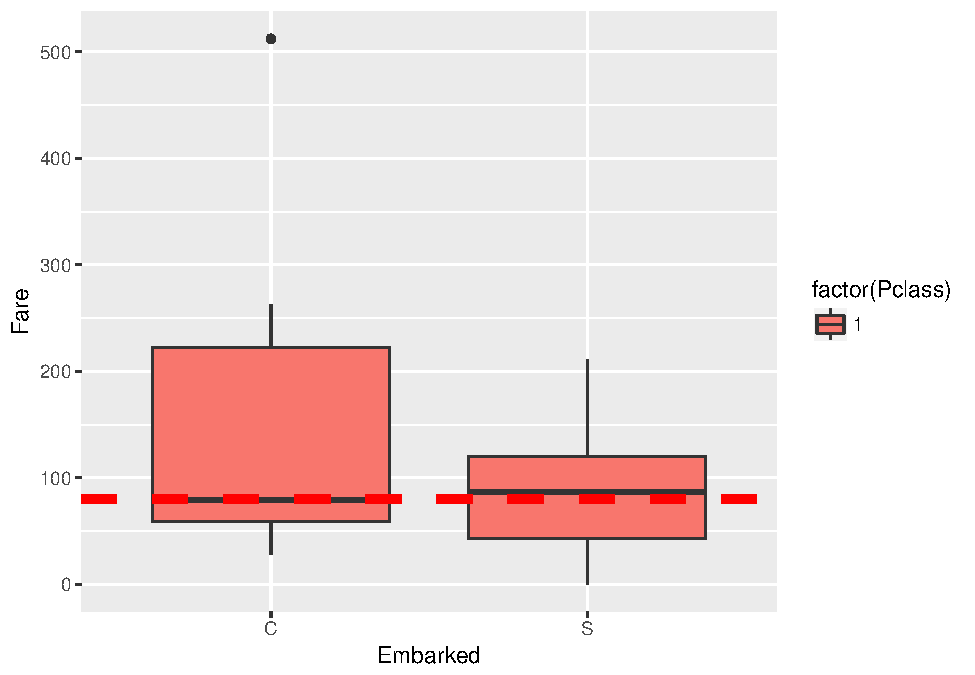
\includegraphics{titanicDataClean_files/figure-latex/bark-1.pdf}

Puede parecer razonable imputar por la mediana de las tarifas de C
porque ese es el valor más cercano. Sin embargo, si miramos hacia atrás
en la sección de tarifas, vemos que hay un 72,4\% de posibilidades de
que un pasajero determinado se embarque desde S.

\begin{verbatim}
##       C   Q   S 
##   2 168  77 644
\end{verbatim}

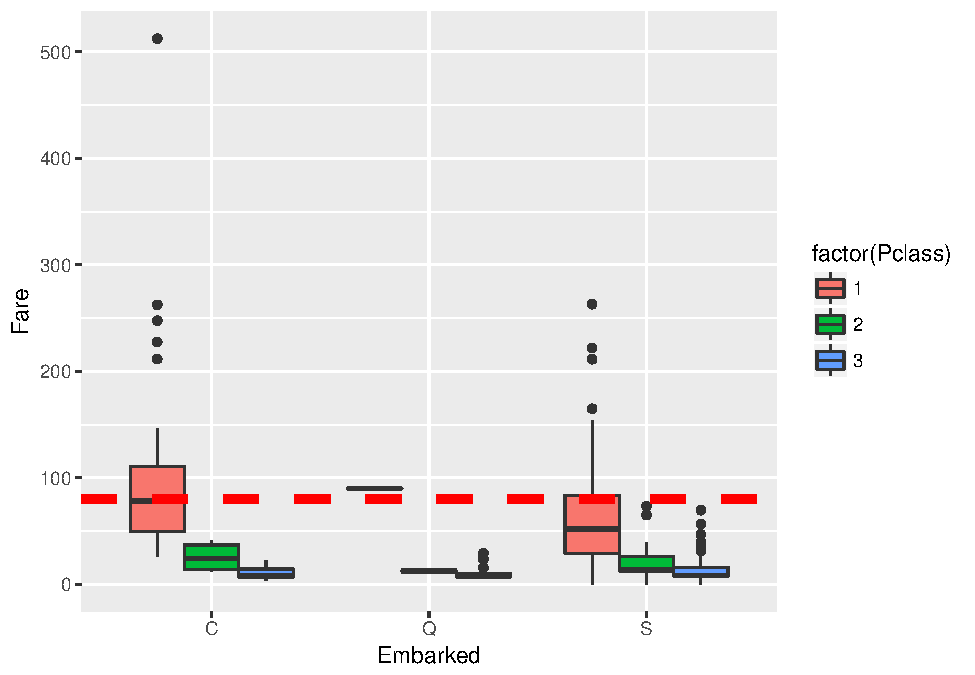
\includegraphics{titanicDataClean_files/figure-latex/split-1.pdf}

\begin{verbatim}
##     C  Q  S 
##  2 22  0 23
\end{verbatim}

Al final, decidí ampliar `S' a la variable y ver dónde eso nos conduce
en el análisis posterior.

\begin{Shaded}
\begin{Highlighting}[]
\NormalTok{titanic_train}\OperatorTok{$}\NormalTok{Embarked[}\KeywordTok{c}\NormalTok{(}\DecValTok{62}\NormalTok{, }\DecValTok{830}\NormalTok{)] <-}\StringTok{ 'S'}
\end{Highlighting}
\end{Shaded}

\section{Análisis de las variables del dataset
titanic}\label{analisis-de-las-variables-del-dataset-titanic}

Para los fines de este estudio, trabajamos con solo cuatro variables de
entrada y una variable de respuesta. Como se mencionó anteriormente, las
cuatro variables de entrada son Class, Sex, Age y Puerto de Embarque. La
variable de respuesta es si sobrevivieron o no.

Podemos recortar los datos según nuestras necesidades usando los
siguientes comandos:

\begin{Shaded}
\begin{Highlighting}[]
\NormalTok{df =}\StringTok{ }\NormalTok{titanic_train[,}\KeywordTok{c}\NormalTok{(}\DecValTok{1}\NormalTok{,}\DecValTok{2}\NormalTok{,}\DecValTok{4}\NormalTok{,}\DecValTok{5}\NormalTok{,}\DecValTok{11}\NormalTok{)]}
\end{Highlighting}
\end{Shaded}

También hacemos que Age sea una variable categórica de la siguiente
manera:

\begin{itemize}
\tightlist
\item
  Si age \textless{}= 18, entonces age = child
\item
  Si 18 \textless{} age \textless{}= 60, entonces age = adult
\item
  Si age \textgreater{} 60, entonces age = senior
\end{itemize}

\begin{Shaded}
\begin{Highlighting}[]
\NormalTok{df}\OperatorTok{$}\NormalTok{Age[df}\OperatorTok{$}\NormalTok{Age }\OperatorTok{<=}\StringTok{ }\DecValTok{18}\NormalTok{] =}\StringTok{ "child"}
\NormalTok{df}\OperatorTok{$}\NormalTok{Age[(df}\OperatorTok{$}\NormalTok{Age }\OperatorTok{>}\StringTok{ }\DecValTok{18}\NormalTok{) }\OperatorTok{&}\StringTok{ }\NormalTok{(df}\OperatorTok{$}\NormalTok{Age }\OperatorTok{<=}\StringTok{ }\DecValTok{60}\NormalTok{) }\OperatorTok{&}\StringTok{ }\NormalTok{(df}\OperatorTok{$}\NormalTok{Age }\OperatorTok{!=}\StringTok{ "child"}\NormalTok{)] =}\StringTok{ "adult"}
\NormalTok{df}\OperatorTok{$}\NormalTok{Age[(df}\OperatorTok{$}\NormalTok{Age }\OperatorTok{!=}\StringTok{ "child"}\NormalTok{) }\OperatorTok{&}\StringTok{ }\NormalTok{(df}\OperatorTok{$}\NormalTok{Age }\OperatorTok{!=}\StringTok{ "adult"}\NormalTok{)] =}\StringTok{ "senior"}
\NormalTok{df}\OperatorTok{$}\NormalTok{Age =}\StringTok{ }\KeywordTok{as.factor}\NormalTok{(df}\OperatorTok{$}\NormalTok{Age)}
\end{Highlighting}
\end{Shaded}

Después de realizar esta operación, nuestros datos se ven así:

\begin{longtable}[]{@{}rrrrr@{}}
\caption{Dataset seleccionado}\tabularnewline
\toprule
Survived & Pclass & Sex & Age & Embarked\tabularnewline
\midrule
\endfirsthead
\toprule
Survived & Pclass & Sex & Age & Embarked\tabularnewline
\midrule
\endhead
0 & 3 & male & adult & S\tabularnewline
1 & 1 & female & adult & C\tabularnewline
1 & 3 & female & adult & S\tabularnewline
1 & 1 & female & adult & S\tabularnewline
0 & 3 & male & adult & S\tabularnewline
0 & 3 & male & adult & Q\tabularnewline
\bottomrule
\end{longtable}

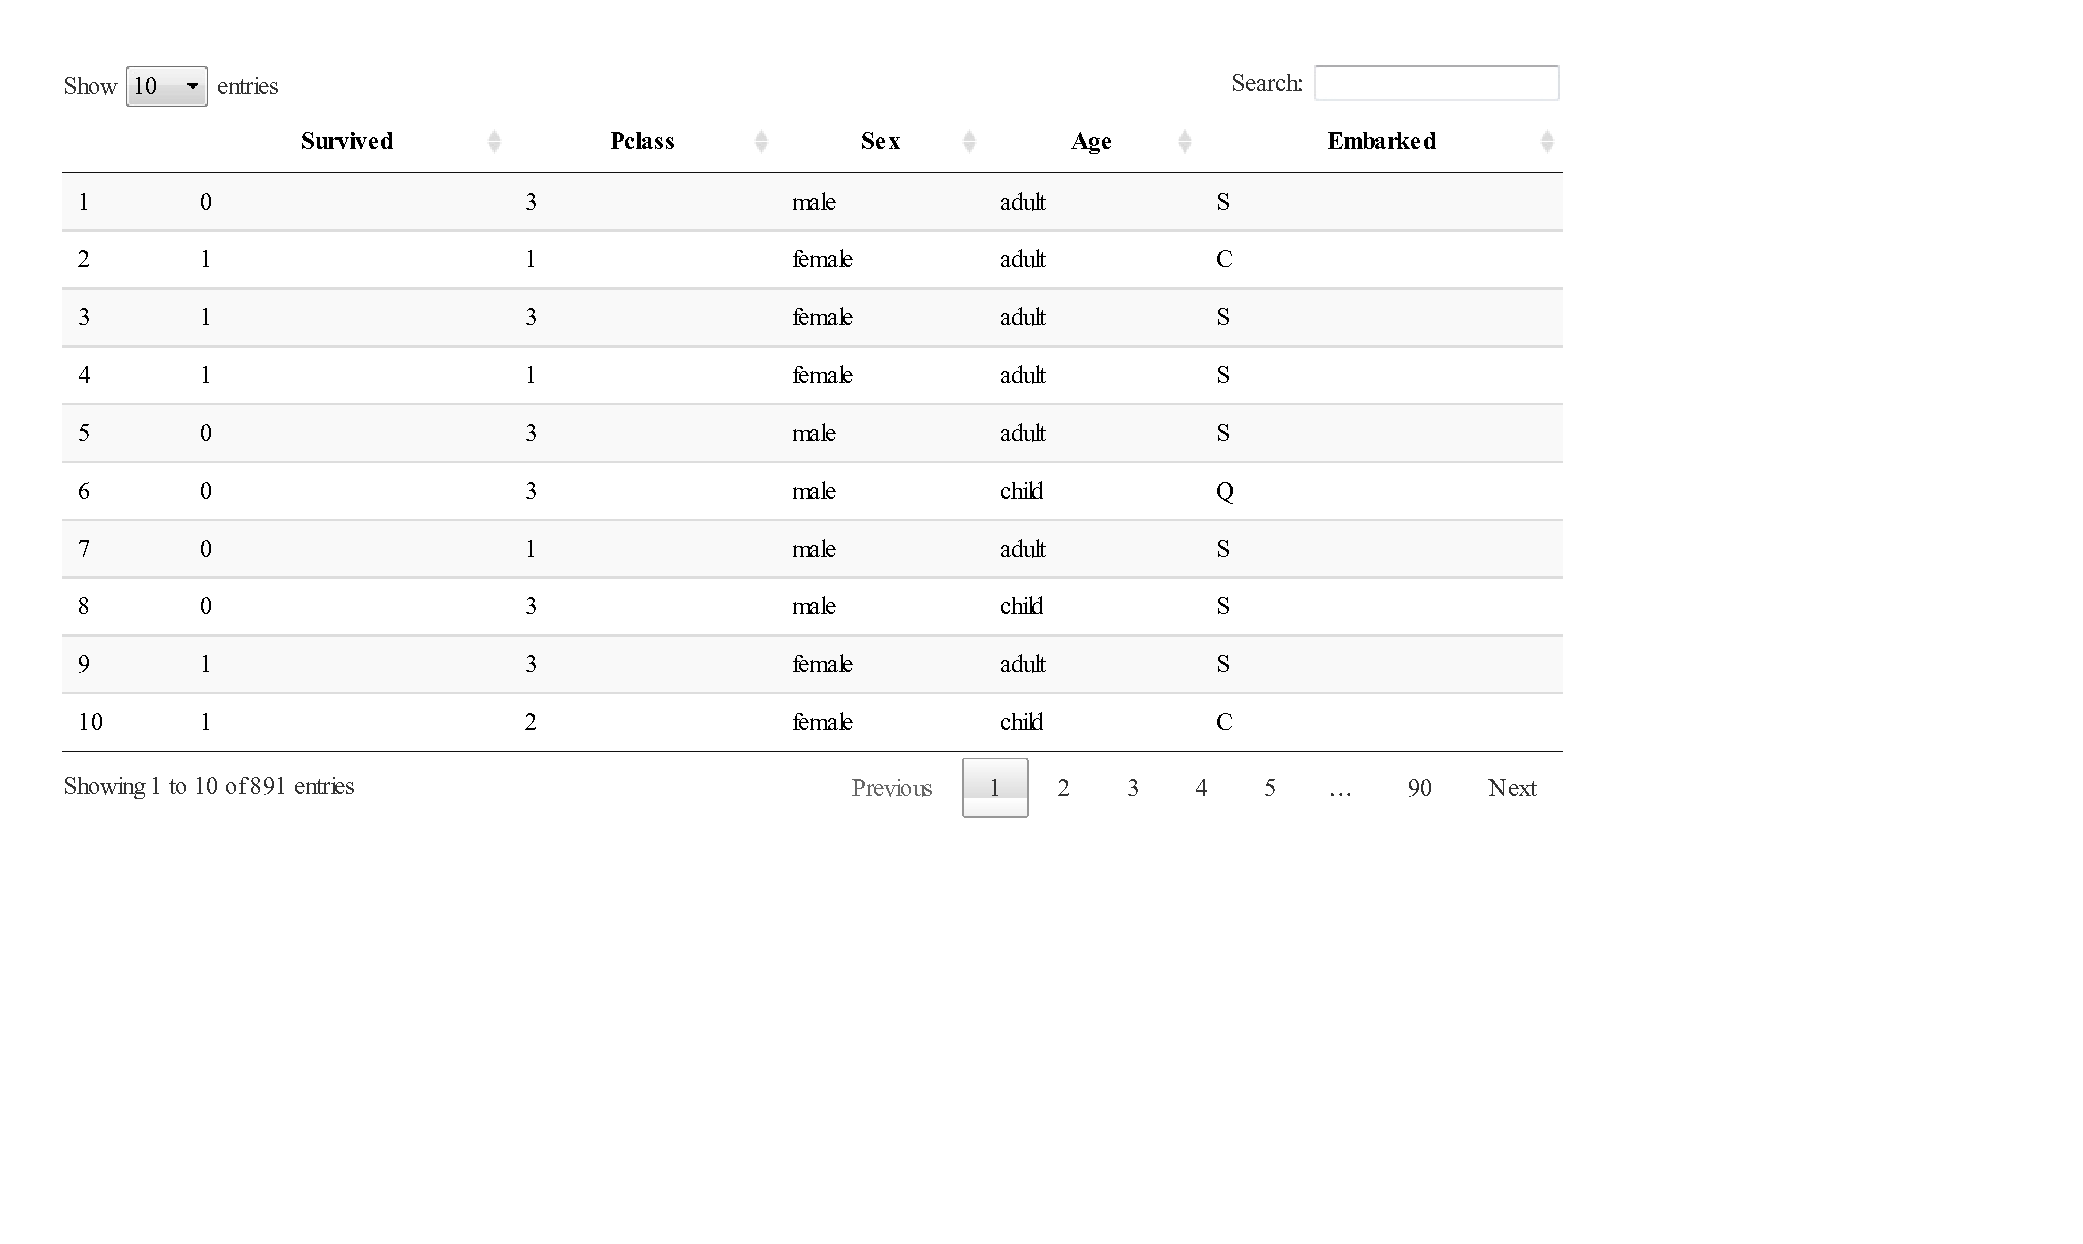
\includegraphics{titanicDataClean_files/figure-latex/class_2-1.pdf}

\begin{Shaded}
\begin{Highlighting}[]
\KeywordTok{summary}\NormalTok{(df)}
\end{Highlighting}
\end{Shaded}

\begin{verbatim}
##  Survived Pclass      Sex          Age      Embarked
##  0:549    1:216   female:314   adult :689    :  0   
##  1:342    2:184   male  :577   child :175   C:168   
##           3:491                senior: 27   Q: 77   
##                                             S:646
\end{verbatim}

\subsection{Diseño experimental}\label{diseno-experimental}

El análisis de datos está organizado de la siguiente manera:

\begin{itemize}
\tightlist
\item
  Computing efectos principales para los cuatro factores
\item
  Computing efectos de interacción para los seis pares de factores
  Análisis computarizado de la varianza (ANOVA) para los cuatro efectos
  principales y los seis efectos de interacción.
\end{itemize}

\subsubsection{Justificación del diseño}\label{justificacion-del-diseno}

La justificación racional detrás de este diseño es la siguiente.
Claramente, tenemos un conjunto de datos a mano que se compone de cuatro
variables de entrada, tres de las cuales son categóricas y la cuarta es
numérica discreta. La variable de respuesta también es categórica.

Lo primero que se me ocurre es analizar individualmente el efecto de
cada una de las variables de entrada en la variable de respuesta. Esto
no es más que calcular los efectos principales.

El segundo nivel de investigación que se me ocurre es comprobar si un
par de dos factores tiene un efecto sinérgico en la variable de
respuesta que parece ser más que el efecto combinado de los dos
factores. Esto no es más que computar los efectos de interacción.

En tercer lugar, desde un punto de vista puramente estadístico, estamos
tratando con muestras de cuatro variables aleatorias como entradas. Si
solo tuviéramos muestras de dos variables aleatorias, habríamos optado
por una prueba z o una prueba t. Sin embargo, dado que hay más de dos
variables aleatorias, se prefiere ANOVA, ya que hace exactamente eso.

Las siguientes subsecciones arrojan luz sobre los temas de
aleatorización, Replicación y Medidas repetidas, y Bloqueo desde un
punto de vista puramente teórico, así como desde el punto de vista de
este estudio.

\subsubsection{Aleatorización}\label{aleatorizacion}

La aleatorización se realiza para permitir la mayor fiabilidad y validez
de las estimaciones estadísticas de los efectos del tratamiento. Más
precisamente, se refiere a asignar aleatoriamente las unidades
experimentales a través de los grupos de tratamiento. La aleatorización
reduce el sesgo al minimizar el efecto de los factores de molestia o el
ruido estocástico en los datos.

En este estudio, los pasajeros del Titanic se dividieron en tres clases
separadas, determinadas por su precio de boleto y su riqueza y clase
social. Los pasajeros en primera clase eran los más ricos del lote e
incluían personas prominentes de clase alta, hombres de negocios,
políticos, personal militar de alto rango, industriales, banqueros, etc.
Los pasajeros de segunda clase incluían profesores, autores, clérigos,
turistas, etc. Pasajeros en tercera clase fueron emigrantes que se
mudaron a los Estados Unidos y Canadá. Además, los pasajeros fueron
variados en etnia también. Hubo pasajeros del Imperio Otomano, otros
tenían orígenes árabes, etc. Por lo tanto, para los fines de este
estudio, hubo una buena cantidad de aleatorización de los pasajeros en
función de su nacionalidad, etnia, condición económica, condición
social, riqueza, etc.

\subsubsection{Replicación y / o medidas
repetidas}\label{replicacion-y-o-medidas-repetidas}

La replicación se refiere a la repetición de un experimento para reducir
la variabilidad asociada con el fenómeno que se estudia. En cualquier
proceso de muestreo, la variación que es inherente no se puede eliminar,
pero lo mejor que se puede hacer es eliminar la variación causada por
causas especiales. Esto es lo que se logra mediante la Replicación.

Hay una línea delgada que separa la replicación de medidas repetidas. La
medición repetida se refiere al uso de los mismos sujetos dentro de cada
rama del estudio, incluido el grupo de control.

En este estudio, los datos disponibles están escritos en piedra.
Realizar la replicación significaría hacer que el barco del Titanic
navegue varias veces y recopilar los datos en todos esos viajes: algunos
de los cuales pueden hundirse y otros no. Realizar medidas repetidas
significaría hacer que la nave del Titanic navegue en un número de
universos paralelos con el mismo grupo de pasajeros. Claramente, ambos
no son prácticos y, por lo tanto, en nuestro estudio, no hay evidencia
de replicación o medidas repetidas.

\subsubsection{Bloqueo}\label{bloqueo}

El bloqueo se refiere a organizar unidades experimentales en grupos
(bloques) que son similares entre sí de alguna manera, forma o forma.
Estos bloques se analizan juntos para reducir la variabilidad conocida.
La idea principal detrás del bloqueo es que una variabilidad que ocurre
en cualquiera de las variables de entrada que no se pueden superar se
confunde con una interacción para eliminar su influencia en la variable
de respuesta.

La base teórica para el bloqueo se puede entender a partir de la
siguiente ecuación. Dadas dos variables aleatorias X e Y,

Var (X-Y) = Var (X) + Var (Y) -2Cov (X, Y)

La varianza de la diferencia se puede minimizar maximizando la
covarianza (o la correlación) entre X e Y.

En este estudio, hemos analizado los datos como un todo porque no había
ninguna razón para sospechar la existencia de variabilidad conocida para
ninguna de las variables de entrada consideradas.

\subsection{Análisis estadístico}\label{analisis-estadistico}

\subsubsection{Análisis exploratorio de
datos}\label{analisis-exploratorio-de-datos}

Resumen de los datos limpios:

\begin{Shaded}
\begin{Highlighting}[]
\KeywordTok{summary}\NormalTok{(df)}
\end{Highlighting}
\end{Shaded}

\begin{verbatim}
##  Survived Pclass      Sex          Age      Embarked
##  0:549    1:216   female:314   adult :689    :  0   
##  1:342    2:184   male  :577   child :175   C:168   
##           3:491                senior: 27   Q: 77   
##                                             S:646
\end{verbatim}

Visualizamos los histogramas de las cuatro variables de entrada:

\begin{Shaded}
\begin{Highlighting}[]
\KeywordTok{barplot}\NormalTok{(}\KeywordTok{table}\NormalTok{(df}\OperatorTok{$}\NormalTok{Pclass), }\DataTypeTok{xlab=}\StringTok{"Class"}\NormalTok{, }\DataTypeTok{ylab=}\StringTok{"Frequency"}\NormalTok{, }\DataTypeTok{main=}\StringTok{"Histograma de Passenger Class"}\NormalTok{)}
\end{Highlighting}
\end{Shaded}

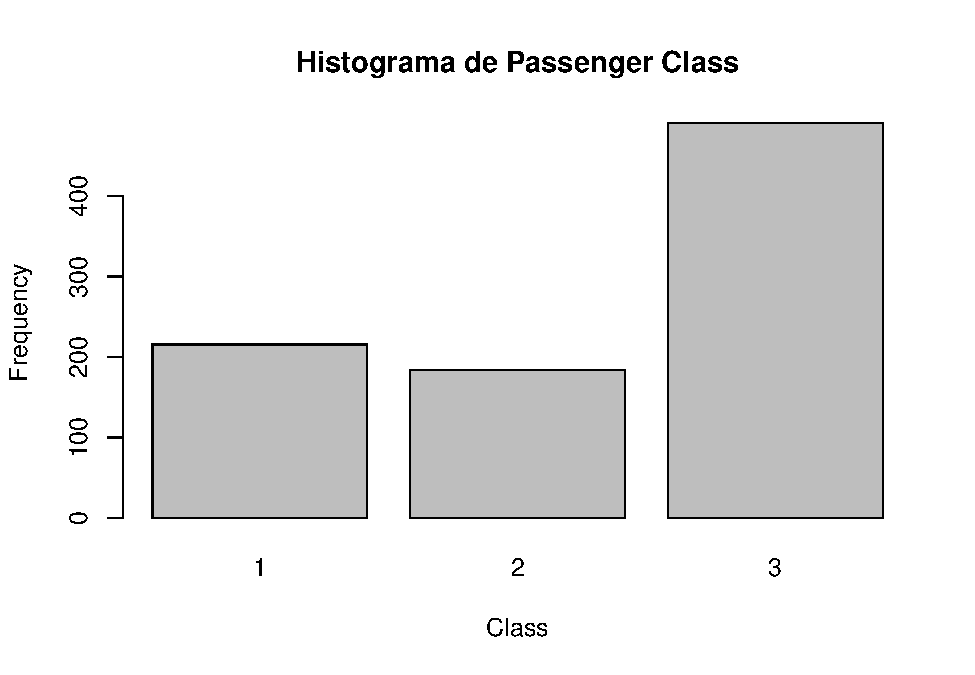
\includegraphics{titanicDataClean_files/figure-latex/unnamed-chunk-11-1.pdf}

\begin{Shaded}
\begin{Highlighting}[]
\KeywordTok{barplot}\NormalTok{(}\KeywordTok{table}\NormalTok{(df}\OperatorTok{$}\NormalTok{Sex), }\DataTypeTok{xlab=}\StringTok{"Sex"}\NormalTok{, }\DataTypeTok{ylab=}\StringTok{"Frequencia"}\NormalTok{, }\DataTypeTok{main=}\StringTok{"Histograma de Sex"}\NormalTok{)}
\end{Highlighting}
\end{Shaded}

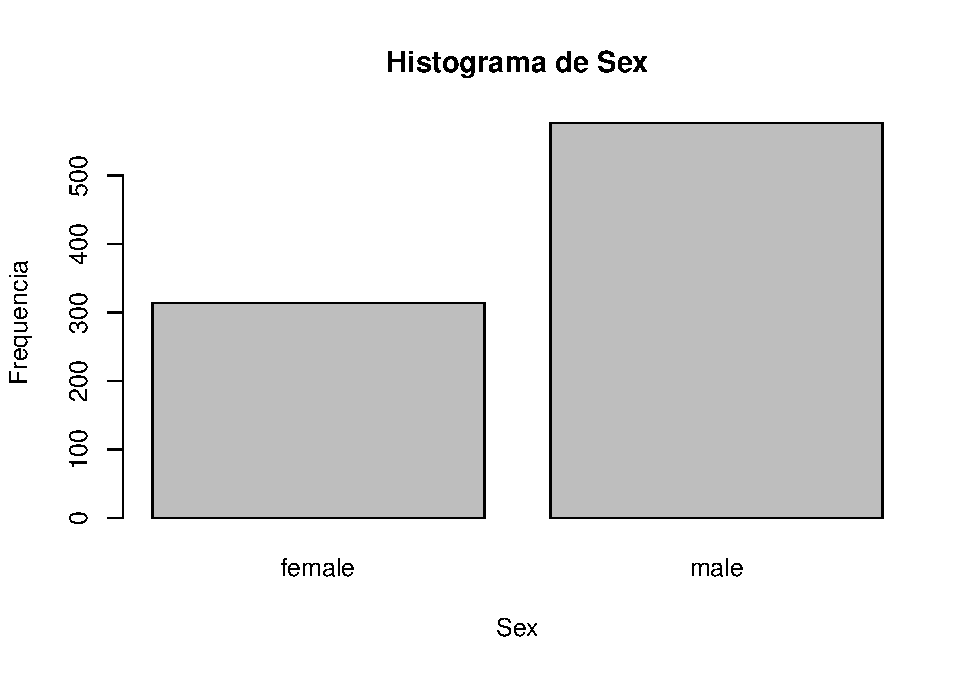
\includegraphics{titanicDataClean_files/figure-latex/unnamed-chunk-11-2.pdf}

\begin{Shaded}
\begin{Highlighting}[]
\KeywordTok{barplot}\NormalTok{(}\KeywordTok{table}\NormalTok{(df}\OperatorTok{$}\NormalTok{Age), }\DataTypeTok{xlab=}\StringTok{"Age"}\NormalTok{, }\DataTypeTok{ylab=}\StringTok{"Frequencia"}\NormalTok{, }\DataTypeTok{main=}\StringTok{"Histograma de Age"}\NormalTok{)}
\end{Highlighting}
\end{Shaded}

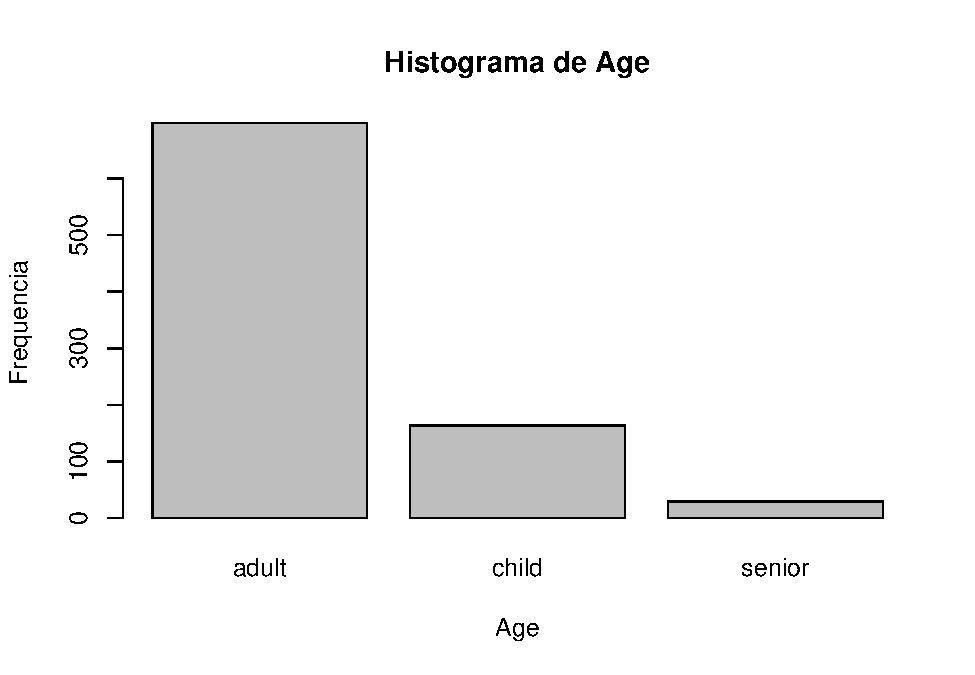
\includegraphics{titanicDataClean_files/figure-latex/unnamed-chunk-11-3.pdf}

\begin{Shaded}
\begin{Highlighting}[]
\KeywordTok{barplot}\NormalTok{(}\KeywordTok{table}\NormalTok{(df}\OperatorTok{$}\NormalTok{Embarked), }\DataTypeTok{xlab=}\StringTok{"Port of Embarkment"}\NormalTok{, }\DataTypeTok{ylab=}\StringTok{"Frequencia"}\NormalTok{, }\DataTypeTok{main=}\StringTok{"Histograma de Port of Embarkment"}\NormalTok{)}
\end{Highlighting}
\end{Shaded}

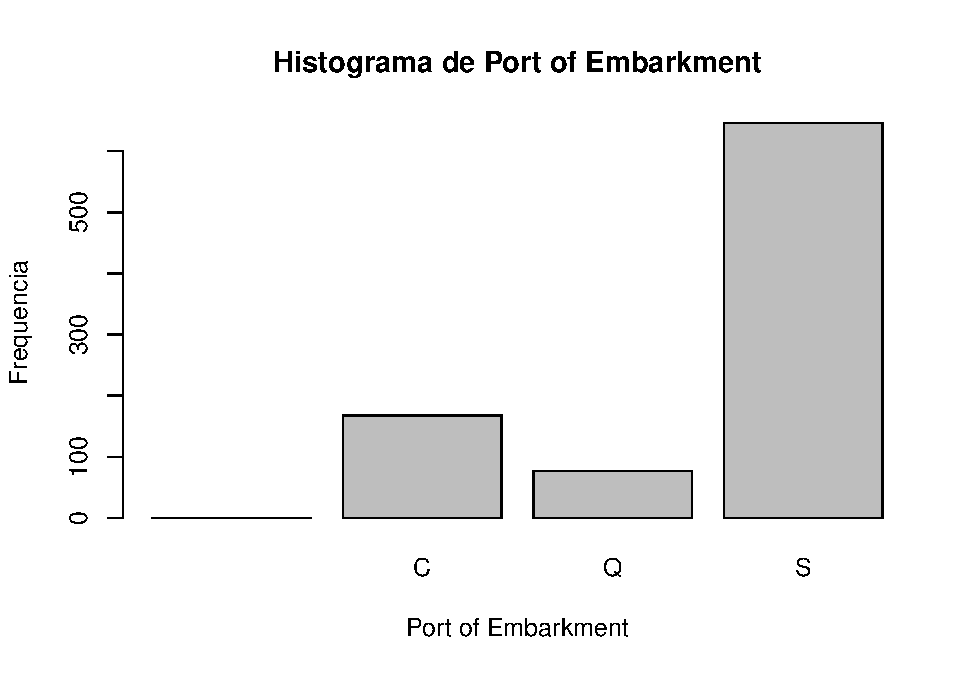
\includegraphics{titanicDataClean_files/figure-latex/unnamed-chunk-11-4.pdf}

\subsubsection{Test}\label{test}

Antes de comenzar con las pruebas, convertimos el dataframe categórico
en un dataframe numérico.

\begin{Shaded}
\begin{Highlighting}[]
\NormalTok{old_df =}\StringTok{ }\NormalTok{df}
\NormalTok{df}\OperatorTok{$}\NormalTok{Pclass =}\StringTok{ }\KeywordTok{as.integer}\NormalTok{(df}\OperatorTok{$}\NormalTok{Pclass)}
\NormalTok{df}\OperatorTok{$}\NormalTok{Sex =}\StringTok{ }\KeywordTok{as.integer}\NormalTok{(df}\OperatorTok{$}\NormalTok{Sex)}
\NormalTok{df}\OperatorTok{$}\NormalTok{Age =}\StringTok{ }\KeywordTok{as.integer}\NormalTok{(df}\OperatorTok{$}\NormalTok{Age)}
\NormalTok{df}\OperatorTok{$}\NormalTok{Embarked =}\StringTok{ }\KeywordTok{as.integer}\NormalTok{(df}\OperatorTok{$}\NormalTok{Embarked)}
\NormalTok{df}\OperatorTok{$}\NormalTok{Survived =}\StringTok{ }\KeywordTok{as.integer}\NormalTok{(df}\OperatorTok{$}\NormalTok{Survived)}
\KeywordTok{head}\NormalTok{(df)}
\end{Highlighting}
\end{Shaded}

\begin{verbatim}
##   Survived Pclass Sex Age Embarked
## 1        1      3   2   1        4
## 2        2      1   1   1        2
## 3        2      3   1   1        4
## 4        2      1   1   1        4
## 5        1      3   2   1        4
## 6        1      3   2   1        3
\end{verbatim}

Parece haber más sobrevivientes en promedio de la 1ra clase en
comparación con los otros dos. El número más bajo de sobrevivientes en
promedio fue de la 3ra clase.

\begin{Shaded}
\begin{Highlighting}[]
\NormalTok{me_pclass =}\StringTok{ }\KeywordTok{c}\NormalTok{(}\DecValTok{0}\NormalTok{,}\DecValTok{0}\NormalTok{,}\DecValTok{0}\NormalTok{)}
\NormalTok{me_pclass[}\DecValTok{1}\NormalTok{] =}\StringTok{ }\KeywordTok{mean}\NormalTok{(df}\OperatorTok{$}\NormalTok{Survived[df}\OperatorTok{$}\NormalTok{Pclass}\OperatorTok{==}\DecValTok{1}\NormalTok{])}
\NormalTok{me_pclass[}\DecValTok{2}\NormalTok{] =}\StringTok{ }\KeywordTok{mean}\NormalTok{(df}\OperatorTok{$}\NormalTok{Survived[df}\OperatorTok{$}\NormalTok{Pclass}\OperatorTok{==}\DecValTok{2}\NormalTok{])}
\NormalTok{me_pclass[}\DecValTok{3}\NormalTok{] =}\StringTok{ }\KeywordTok{mean}\NormalTok{(df}\OperatorTok{$}\NormalTok{Survived[df}\OperatorTok{$}\NormalTok{Pclass}\OperatorTok{==}\DecValTok{3}\NormalTok{])}
\KeywordTok{plot}\NormalTok{(me_pclass, }\DataTypeTok{type=}\StringTok{"o"}\NormalTok{, }\DataTypeTok{main=}\StringTok{"Efecto principal de Passenger Class"}\NormalTok{, }\DataTypeTok{xlab=}\StringTok{"Passenger Class"}\NormalTok{, }\DataTypeTok{ylab=}\StringTok{"Efecto principal"}\NormalTok{,}
     \DataTypeTok{xaxt=}\StringTok{"n"}\NormalTok{)}
\KeywordTok{axis}\NormalTok{(}\DecValTok{1}\NormalTok{, }\DataTypeTok{at=}\KeywordTok{c}\NormalTok{(}\DecValTok{1}\NormalTok{,}\DecValTok{2}\NormalTok{,}\DecValTok{3}\NormalTok{), }\DataTypeTok{labels=}\KeywordTok{c}\NormalTok{(}\StringTok{"1er"}\NormalTok{, }\StringTok{"2nd"}\NormalTok{, }\StringTok{"3er"}\NormalTok{))}
\end{Highlighting}
\end{Shaded}

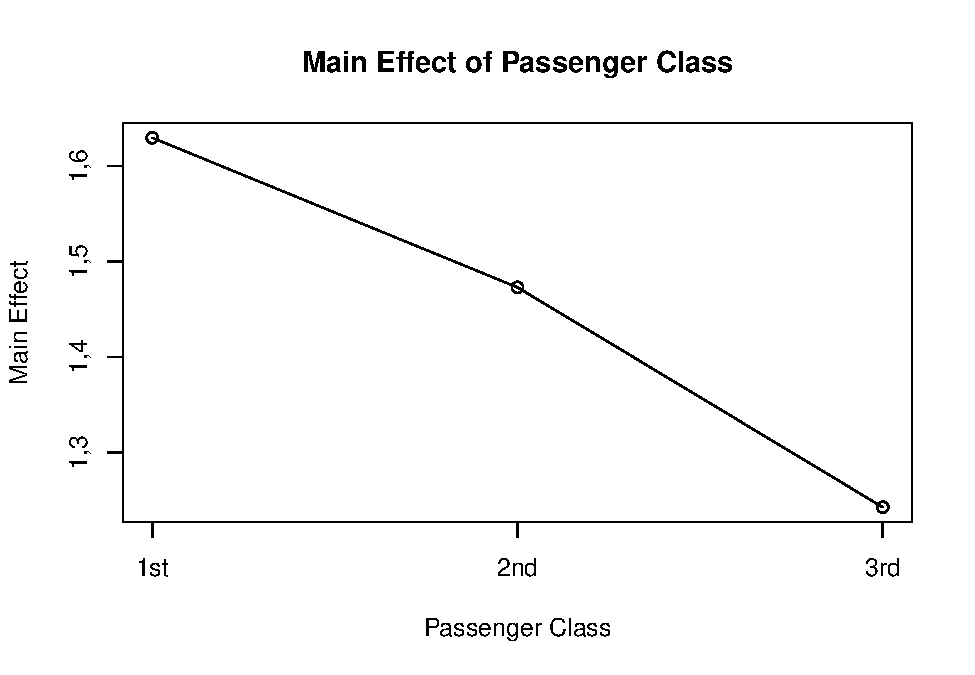
\includegraphics{titanicDataClean_files/figure-latex/unnamed-chunk-13-1.pdf}

Las sobrevivientes femeninas eran mucho más numerosas que los hombres.

\begin{Shaded}
\begin{Highlighting}[]
\NormalTok{me_sex =}\StringTok{ }\KeywordTok{c}\NormalTok{(}\DecValTok{0}\NormalTok{,}\DecValTok{0}\NormalTok{)}
\NormalTok{me_sex[}\DecValTok{1}\NormalTok{] =}\StringTok{ }\KeywordTok{mean}\NormalTok{(df}\OperatorTok{$}\NormalTok{Survived[df}\OperatorTok{$}\NormalTok{Sex}\OperatorTok{==}\DecValTok{1}\NormalTok{])}
\NormalTok{me_sex[}\DecValTok{2}\NormalTok{] =}\StringTok{ }\KeywordTok{mean}\NormalTok{(df}\OperatorTok{$}\NormalTok{Survived[df}\OperatorTok{$}\NormalTok{Sex}\OperatorTok{==}\DecValTok{2}\NormalTok{])}
\KeywordTok{plot}\NormalTok{(me_sex, }\DataTypeTok{type=}\StringTok{"o"}\NormalTok{, }\DataTypeTok{main=}\StringTok{"Efecto principal de Sex"}\NormalTok{, }\DataTypeTok{xlab=}\StringTok{"Sex"}\NormalTok{, }\DataTypeTok{ylab=}\StringTok{"Efecto principal"}\NormalTok{, }\DataTypeTok{xaxt=}\StringTok{"n"}\NormalTok{)}
\KeywordTok{axis}\NormalTok{(}\DecValTok{1}\NormalTok{, }\DataTypeTok{at=}\KeywordTok{c}\NormalTok{(}\DecValTok{1}\NormalTok{,}\DecValTok{2}\NormalTok{), }\DataTypeTok{labels=}\KeywordTok{c}\NormalTok{(}\StringTok{"Mujer"}\NormalTok{, }\StringTok{"Hombre"}\NormalTok{))}
\end{Highlighting}
\end{Shaded}

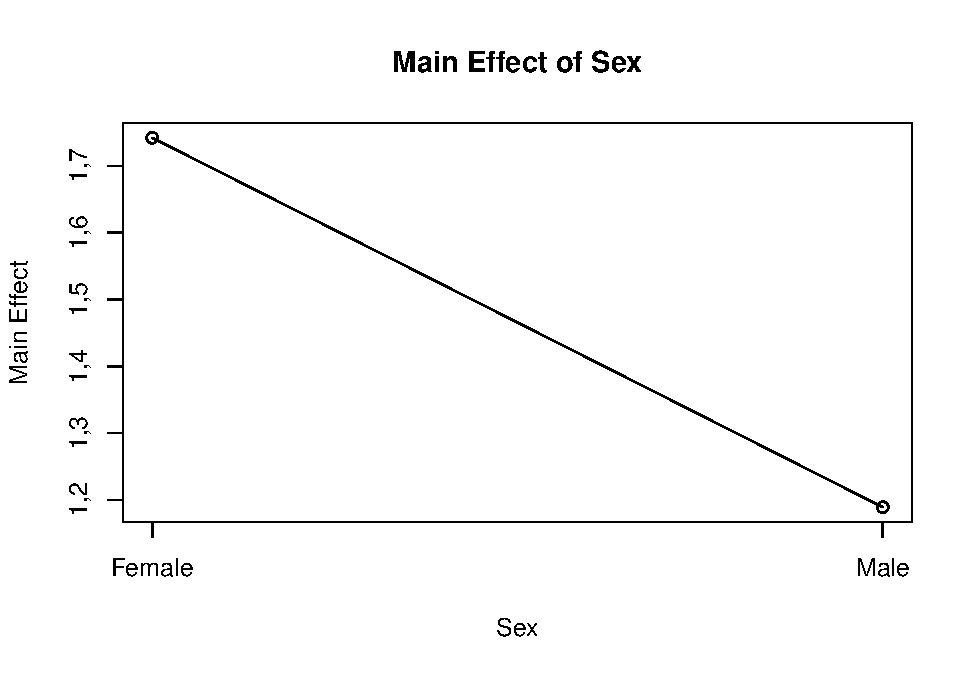
\includegraphics{titanicDataClean_files/figure-latex/unnamed-chunk-14-1.pdf}

Los supervivientes máximos en promedio de la categoría de edad eran
niños, seguidos de adultos y personas mayores.

\begin{Shaded}
\begin{Highlighting}[]
\NormalTok{me_age =}\StringTok{ }\KeywordTok{c}\NormalTok{(}\DecValTok{0}\NormalTok{,}\DecValTok{0}\NormalTok{,}\DecValTok{0}\NormalTok{)}
\NormalTok{me_age[}\DecValTok{1}\NormalTok{] =}\StringTok{ }\KeywordTok{mean}\NormalTok{(df}\OperatorTok{$}\NormalTok{Survived[df}\OperatorTok{$}\NormalTok{Age}\OperatorTok{==}\DecValTok{1}\NormalTok{])}
\NormalTok{me_age[}\DecValTok{2}\NormalTok{] =}\StringTok{ }\KeywordTok{mean}\NormalTok{(df}\OperatorTok{$}\NormalTok{Survived[df}\OperatorTok{$}\NormalTok{Age}\OperatorTok{==}\DecValTok{2}\NormalTok{])}
\NormalTok{me_age[}\DecValTok{3}\NormalTok{] =}\StringTok{ }\KeywordTok{mean}\NormalTok{(df}\OperatorTok{$}\NormalTok{Survived[df}\OperatorTok{$}\NormalTok{Age}\OperatorTok{==}\DecValTok{3}\NormalTok{])}
\KeywordTok{plot}\NormalTok{(me_age, }\DataTypeTok{type=}\StringTok{"o"}\NormalTok{, }\DataTypeTok{main=}\StringTok{"Efecto principal de Age"}\NormalTok{, }\DataTypeTok{xlab=}\StringTok{"Age"}\NormalTok{, }\DataTypeTok{ylab=}\StringTok{"Efecto principal"}\NormalTok{, }\DataTypeTok{xaxt=}\StringTok{"n"}\NormalTok{)}
\KeywordTok{axis}\NormalTok{(}\DecValTok{1}\NormalTok{, }\DataTypeTok{at=}\KeywordTok{c}\NormalTok{(}\DecValTok{1}\NormalTok{,}\DecValTok{2}\NormalTok{,}\DecValTok{3}\NormalTok{), }\DataTypeTok{labels=}\KeywordTok{c}\NormalTok{(}\StringTok{"Adult"}\NormalTok{, }\StringTok{"Children"}\NormalTok{, }\StringTok{"Senior Citizen"}\NormalTok{))}
\end{Highlighting}
\end{Shaded}

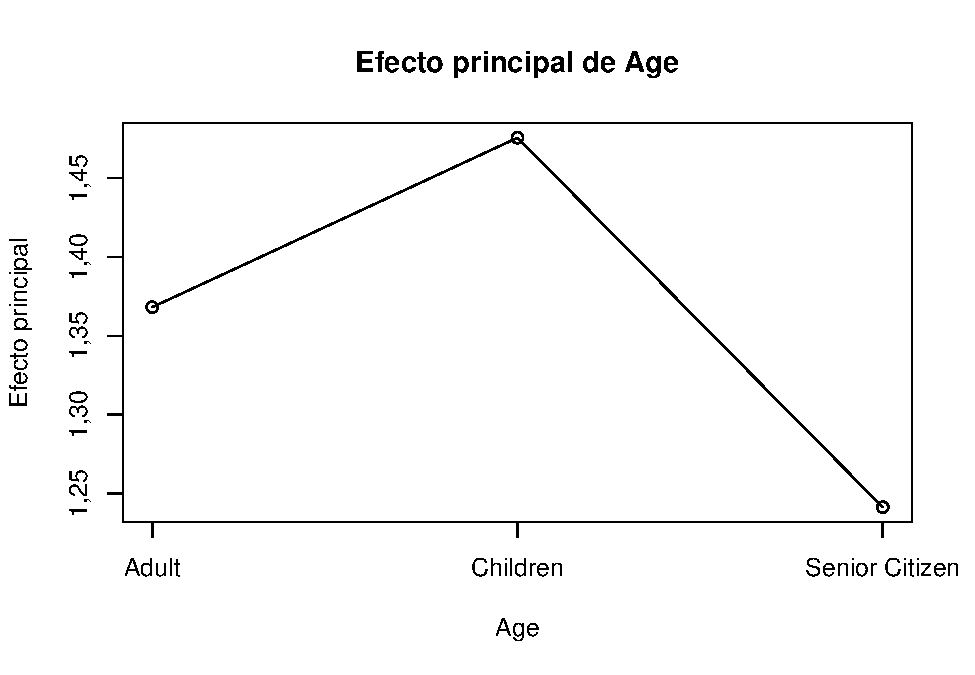
\includegraphics{titanicDataClean_files/figure-latex/unnamed-chunk-15-1.pdf}

La gente que abordó el Titanic en Cherbourg tenía el número máximo de
supervivientes en promedio, seguidos de los que abordaron el barco en
Southampton y finalmente en Queenstown.

\begin{Shaded}
\begin{Highlighting}[]
\NormalTok{me_emb =}\StringTok{ }\KeywordTok{c}\NormalTok{(}\DecValTok{0}\NormalTok{,}\DecValTok{0}\NormalTok{,}\DecValTok{0}\NormalTok{)}
\NormalTok{me_emb[}\DecValTok{1}\NormalTok{] =}\StringTok{ }\KeywordTok{mean}\NormalTok{(df}\OperatorTok{$}\NormalTok{Survived[df}\OperatorTok{$}\NormalTok{Embarked}\OperatorTok{==}\DecValTok{1}\NormalTok{])}
\NormalTok{me_emb[}\DecValTok{2}\NormalTok{] =}\StringTok{ }\KeywordTok{mean}\NormalTok{(df}\OperatorTok{$}\NormalTok{Survived[df}\OperatorTok{$}\NormalTok{Embarked}\OperatorTok{==}\DecValTok{2}\NormalTok{])}
\NormalTok{me_emb[}\DecValTok{3}\NormalTok{] =}\StringTok{ }\KeywordTok{mean}\NormalTok{(df}\OperatorTok{$}\NormalTok{Survived[df}\OperatorTok{$}\NormalTok{Embarked}\OperatorTok{==}\DecValTok{3}\NormalTok{])}
\KeywordTok{plot}\NormalTok{(me_emb, }\DataTypeTok{type=}\StringTok{"o"}\NormalTok{, }\DataTypeTok{main=}\StringTok{"Efecto principal de Port of Embarkment"}\NormalTok{, }\DataTypeTok{xlab=}\StringTok{"Port of Embarkment"}\NormalTok{, }\DataTypeTok{ylab=}\StringTok{"Efecto principal"}\NormalTok{,}
     \DataTypeTok{xaxt=}\StringTok{"n"}\NormalTok{)}
\KeywordTok{axis}\NormalTok{(}\DecValTok{1}\NormalTok{, }\DataTypeTok{at=}\KeywordTok{c}\NormalTok{(}\DecValTok{1}\NormalTok{,}\DecValTok{2}\NormalTok{,}\DecValTok{3}\NormalTok{), }\DataTypeTok{labels=}\KeywordTok{c}\NormalTok{(}\StringTok{"Cherbourg"}\NormalTok{, }\StringTok{"Queenstown"}\NormalTok{, }\StringTok{"Southampton"}\NormalTok{))}
\end{Highlighting}
\end{Shaded}

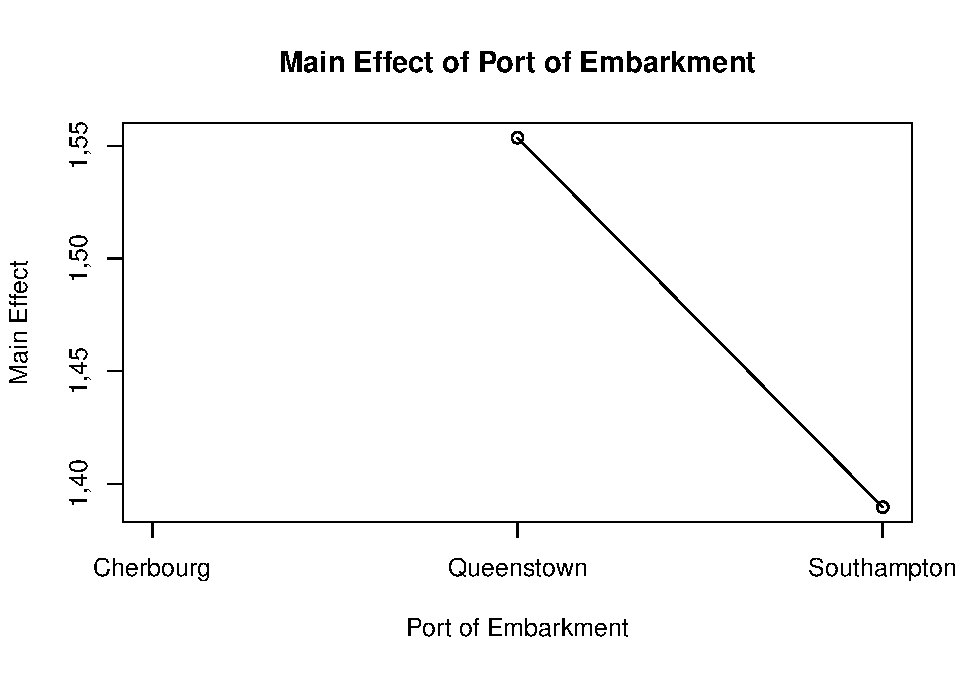
\includegraphics{titanicDataClean_files/figure-latex/unnamed-chunk-16-1.pdf}

Existe un claro efecto de interacción entre la clase de pasajeros y el
sexo. Los pasajeros femeninos de primera y segunda clase tuvieron un
mayor número de sobrevivientes que las pasajeras de tercera clase. Los
pasajeros varones de primera clase tenían un número promedio mayor de
sobrevivientes que los pasajeros masculinos de segunda y tercera clase.

\begin{Shaded}
\begin{Highlighting}[]
\KeywordTok{interaction.plot}\NormalTok{(df}\OperatorTok{$}\NormalTok{Pclass, df}\OperatorTok{$}\NormalTok{Sex, df}\OperatorTok{$}\NormalTok{Survived, }\DataTypeTok{xlab=}\StringTok{"Passenger Class"}\NormalTok{, }\DataTypeTok{ylab=}\StringTok{"Número promedio de sobrevivientes"}\NormalTok{,}
                  \DataTypeTok{main=}\StringTok{"Efecto de interacción entre Passenger Class y Sex"}\NormalTok{, }\DataTypeTok{legend=}\OtherTok{FALSE}\NormalTok{)}
\KeywordTok{legend}\NormalTok{(}\StringTok{"topright"}\NormalTok{, }\KeywordTok{c}\NormalTok{(}\StringTok{"Mujer"}\NormalTok{,}\StringTok{"Hombre"}\NormalTok{), }\DataTypeTok{lty=}\KeywordTok{c}\NormalTok{(}\StringTok{"dashed"}\NormalTok{, }\StringTok{"solid"}\NormalTok{), }\DataTypeTok{title=}\StringTok{"Sex"}\NormalTok{)}
\end{Highlighting}
\end{Shaded}

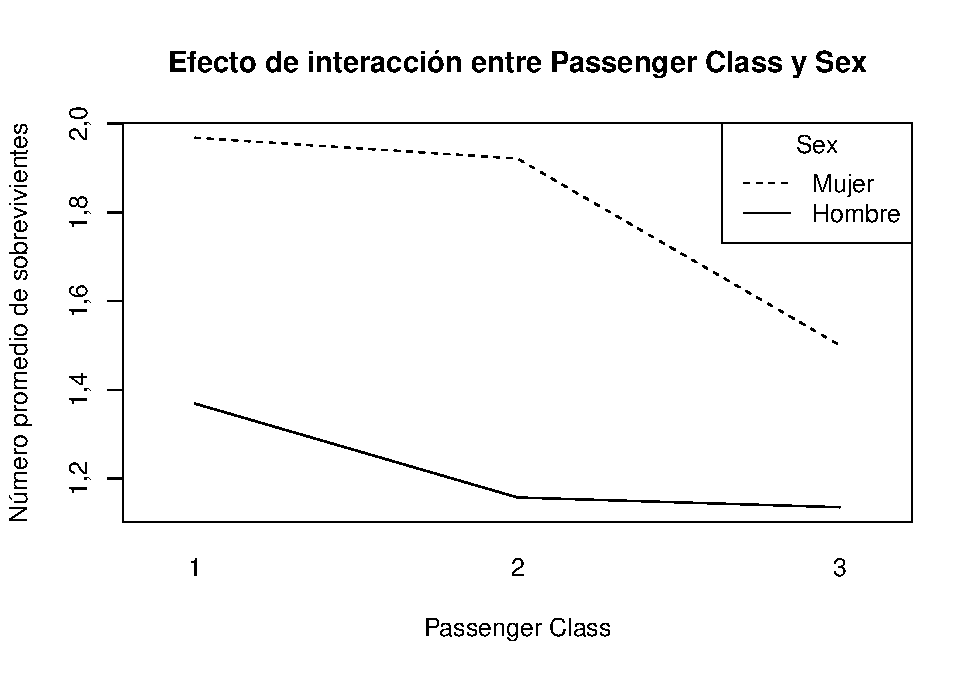
\includegraphics{titanicDataClean_files/figure-latex/unnamed-chunk-17-1.pdf}

Hay un efecto de interacción entre la clase de pasajero y la edad. En
general, los adultos tenían una media de sobrevivientes mejor que las
personas mayores, que eran mejores que los niños. Más adultos de 1ra
clase sobrevivieron que la 2da clase, que tuvo más sobrevivientes que la
3ra clase. Lo mismo es la tendencia para las personas mayores también.
Sin embargo, el número promedio de sobrevivientes fue más alto para los
niños de 2a clase y el más bajo para los niños de 1ra clase.

\begin{Shaded}
\begin{Highlighting}[]
\KeywordTok{interaction.plot}\NormalTok{(df}\OperatorTok{$}\NormalTok{Pclass, df}\OperatorTok{$}\NormalTok{Age, df}\OperatorTok{$}\NormalTok{Survived, }\DataTypeTok{xlab=}\StringTok{"Passenger Class"}\NormalTok{, }\DataTypeTok{ylab=}\StringTok{"Número promedio de sobrevivientes"}\NormalTok{,}
                 \DataTypeTok{main=}\StringTok{"Efecto de interacción entre Passenger Class y Age"}\NormalTok{, }\DataTypeTok{legend=}\OtherTok{FALSE}\NormalTok{)}
\KeywordTok{legend}\NormalTok{(}\StringTok{"topright"}\NormalTok{, }\KeywordTok{c}\NormalTok{(}\StringTok{"Adult"}\NormalTok{,}\StringTok{"Child"}\NormalTok{, }\StringTok{"Senior"}\NormalTok{), }\DataTypeTok{lty=}\KeywordTok{c}\NormalTok{(}\StringTok{"dashed"}\NormalTok{, }\StringTok{"solid"}\NormalTok{, }\StringTok{"dotted"}\NormalTok{), }\DataTypeTok{title=}\StringTok{"Age"}\NormalTok{)}
\end{Highlighting}
\end{Shaded}

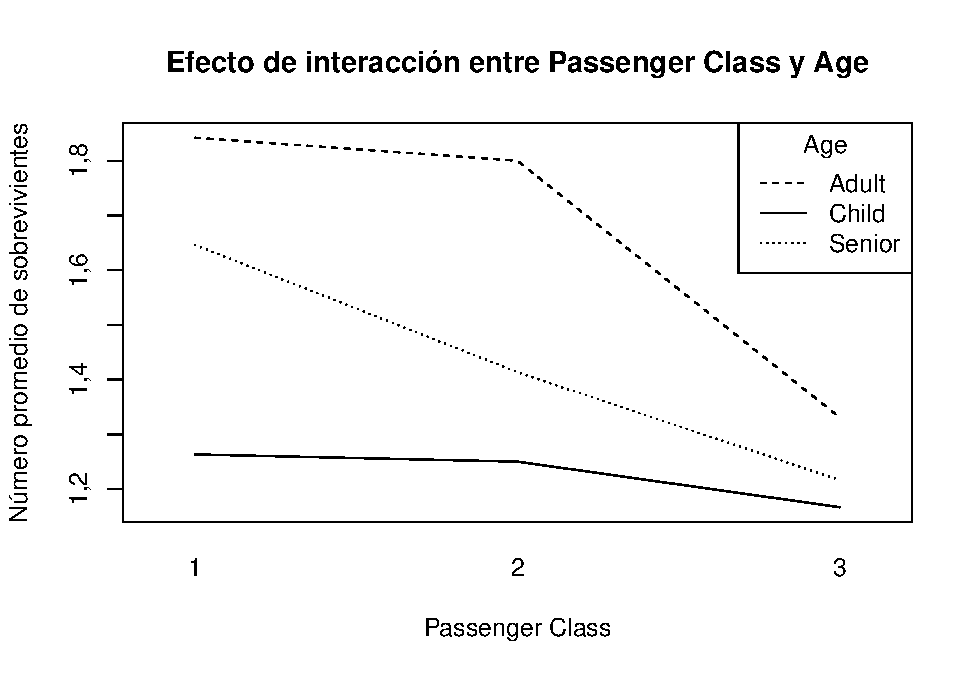
\includegraphics{titanicDataClean_files/figure-latex/unnamed-chunk-18-1.pdf}

También hay un efecto de interacción entre la Clase de Pasajero y el
Puerto de Embarque. Para los pasajeros que abordaron el barco desde
Queenstown y Southampton, los pasajeros de primera clase sobrevivieron
más y los pasajeros de tercera clase sobrevivieron lo mínimo. Para los
pasajeros que abordaron el barco desde Cherbourg, el número medio de
supervivientes era casi el mismo para los pasajeros de 1ra y 2da clase,
que eran mayores que los pasajeros de 3ra clase. Para los pasajeros de
segunda y tercera clase que abordaron desde Cherbourg y Queenstown, no
parece haber ningún efecto de interacción.

\begin{Shaded}
\begin{Highlighting}[]
\KeywordTok{interaction.plot}\NormalTok{(df}\OperatorTok{$}\NormalTok{Pclass, df}\OperatorTok{$}\NormalTok{Embarked, df}\OperatorTok{$}\NormalTok{Survived, }\DataTypeTok{xlab=}\StringTok{"Passenger Class"}\NormalTok{, }\DataTypeTok{ylab=}\StringTok{"Número promedio de sobrevivientes"}\NormalTok{,}
                 \DataTypeTok{main=}\StringTok{"Efecto de interacción entre Passenger Class y Port of Embarkment"}\NormalTok{, }\DataTypeTok{legend=}\OtherTok{FALSE}\NormalTok{)}
\KeywordTok{legend}\NormalTok{(}\StringTok{"topright"}\NormalTok{, }\KeywordTok{c}\NormalTok{(}\StringTok{"Cherbourg"}\NormalTok{,}\StringTok{"Queenstown"}\NormalTok{,}\StringTok{"Southampton"}\NormalTok{), }\DataTypeTok{lty=}\KeywordTok{c}\NormalTok{(}\StringTok{"dashed"}\NormalTok{, }\StringTok{"solid"}\NormalTok{, }\StringTok{"dotted"}\NormalTok{),}
       \DataTypeTok{title=}\StringTok{"Port of Embarkment"}\NormalTok{)}
\end{Highlighting}
\end{Shaded}

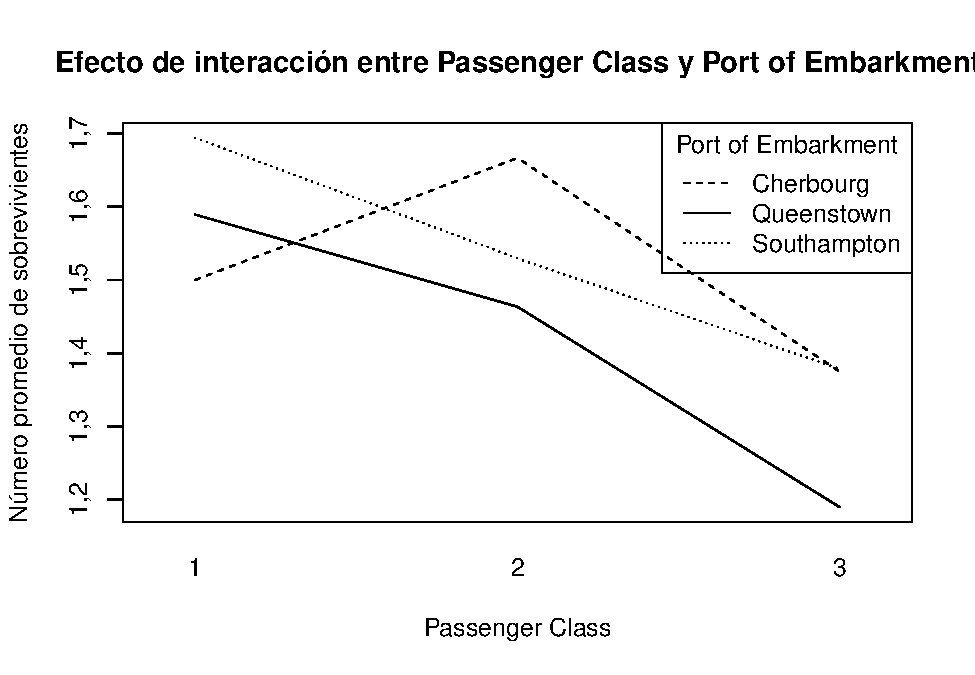
\includegraphics{titanicDataClean_files/figure-latex/unnamed-chunk-19-1.pdf}

Es interesante observar que en un momento tan crítico (cuando el barco
se hundía), el número medio de supervivientes para la 1ra clase era
mucho menor que las otras dos clases. Esto esencialmente refleja y
refuerza su poder y estatura en la sociedad: se les dio la prioridad de
alcanzar la seguridad, incluso en un momento en que todo el barco se
hundía y casi todos tenían una oportunidad sustancial de encontrarse con
su muerte ese día.

Parece haber un efecto de interacción entre la edad y el sexo. Hubo más
sobrevivientes de hombres que adultos varones, que fueron mayores que
los varones. Por el contrario, hubo más sobrevivientes de niñas que
mujeres de la tercera edad, que fueron mayores que las mujeres adultas.
En general, hubo más mujeres supervivientes en comparación con los
hombres en todos los grupos de edad.

\begin{Shaded}
\begin{Highlighting}[]
\KeywordTok{interaction.plot}\NormalTok{(df}\OperatorTok{$}\NormalTok{Sex, df}\OperatorTok{$}\NormalTok{Age, df}\OperatorTok{$}\NormalTok{Survived, }\DataTypeTok{xlab=}\StringTok{"Sex"}\NormalTok{, }\DataTypeTok{ylab=}\StringTok{"Número promedio de sobrevivientes"}\NormalTok{,}
                 \DataTypeTok{main=}\StringTok{"Efecto de interacción entre Sex y Age"}\NormalTok{, }\DataTypeTok{legend=}\OtherTok{FALSE}\NormalTok{, }\DataTypeTok{xtick=}\OtherTok{FALSE}\NormalTok{, }\DataTypeTok{xaxt=}\StringTok{"n"}\NormalTok{)}
\KeywordTok{axis}\NormalTok{(}\DecValTok{1}\NormalTok{, }\KeywordTok{c}\NormalTok{(}\DecValTok{1}\NormalTok{,}\DecValTok{2}\NormalTok{), }\DataTypeTok{labels=}\KeywordTok{c}\NormalTok{(}\StringTok{"Female"}\NormalTok{, }\StringTok{"Male"}\NormalTok{))}
\KeywordTok{legend}\NormalTok{(}\StringTok{"topright"}\NormalTok{, }\KeywordTok{c}\NormalTok{(}\StringTok{"Adult"}\NormalTok{,}\StringTok{"Child"}\NormalTok{, }\StringTok{"Senior"}\NormalTok{), }\DataTypeTok{lty=}\KeywordTok{c}\NormalTok{(}\StringTok{"dashed"}\NormalTok{, }\StringTok{"solid"}\NormalTok{, }\StringTok{"dotted"}\NormalTok{), }\DataTypeTok{title=}\StringTok{"Age"}\NormalTok{)}
\end{Highlighting}
\end{Shaded}

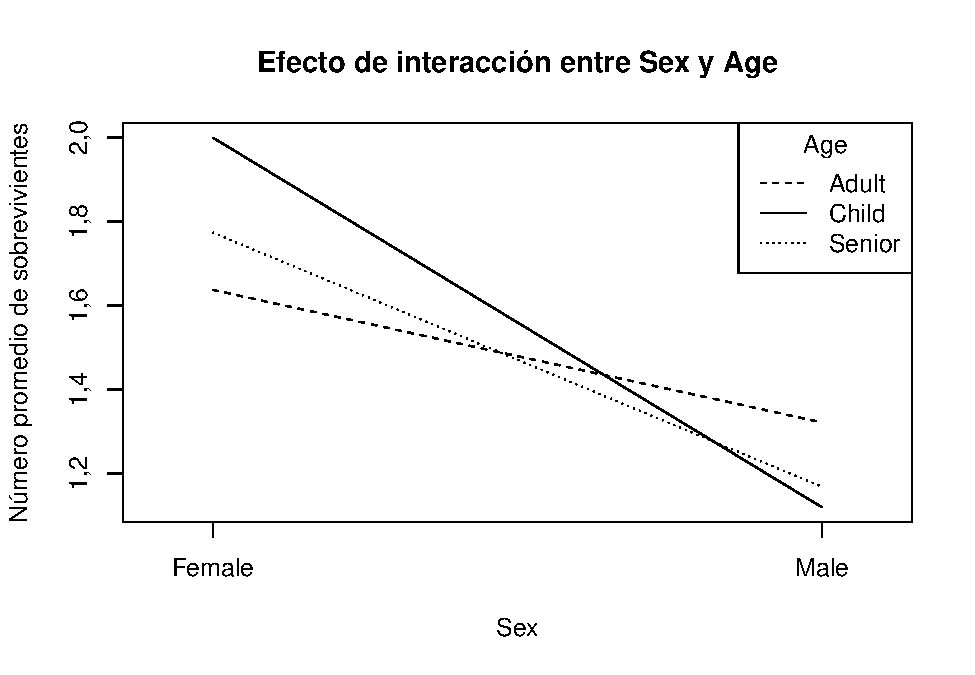
\includegraphics{titanicDataClean_files/figure-latex/unnamed-chunk-20-1.pdf}

No parece haber ningún efecto de interacción entre Sexo y Puerto de
Embarque.

\begin{Shaded}
\begin{Highlighting}[]
\KeywordTok{interaction.plot}\NormalTok{(df}\OperatorTok{$}\NormalTok{Sex, df}\OperatorTok{$}\NormalTok{Embarked, df}\OperatorTok{$}\NormalTok{Survived, }\DataTypeTok{xlab=}\StringTok{"Sex"}\NormalTok{, }\DataTypeTok{ylab=}\StringTok{"Número promedio de sobrevivientes"}\NormalTok{, }
                 \DataTypeTok{main=}\StringTok{"Efecto de interacción entre Sex y Port of Embarkment"}\NormalTok{, }\DataTypeTok{legend=}\OtherTok{FALSE}\NormalTok{, }\DataTypeTok{xtick =} \OtherTok{FALSE}\NormalTok{, }\DataTypeTok{xaxt=}\StringTok{"n"}\NormalTok{)}
\KeywordTok{axis}\NormalTok{(}\DecValTok{1}\NormalTok{, }\KeywordTok{c}\NormalTok{(}\DecValTok{1}\NormalTok{,}\DecValTok{2}\NormalTok{), }\DataTypeTok{labels=}\KeywordTok{c}\NormalTok{(}\StringTok{"Female"}\NormalTok{, }\StringTok{"Male"}\NormalTok{))}
\KeywordTok{legend}\NormalTok{(}\StringTok{"topright"}\NormalTok{, }\KeywordTok{c}\NormalTok{(}\StringTok{"Cherbourg"}\NormalTok{,}\StringTok{"Queenstown"}\NormalTok{,}\StringTok{"Southampton"}\NormalTok{), }\DataTypeTok{lty=}\KeywordTok{c}\NormalTok{(}\StringTok{"dashed"}\NormalTok{, }\StringTok{"solid"}\NormalTok{, }\StringTok{"dotted"}\NormalTok{),}
       \DataTypeTok{title=}\StringTok{"Port of Embarkment"}\NormalTok{)}
\end{Highlighting}
\end{Shaded}

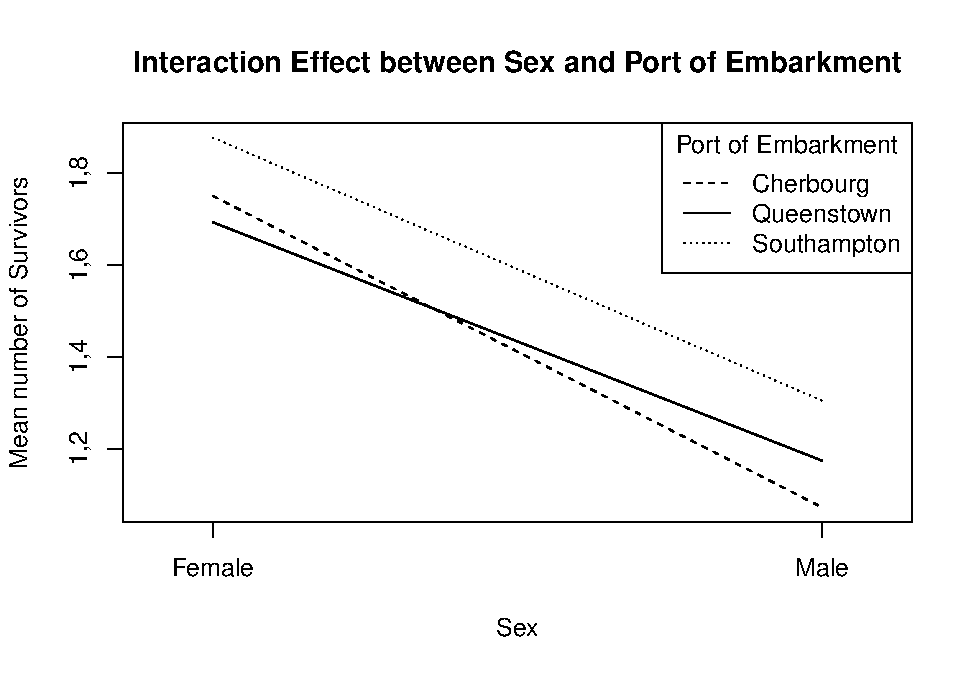
\includegraphics{titanicDataClean_files/figure-latex/unnamed-chunk-21-1.pdf}

Hay un efecto de interacción entre la edad y el puerto de embarque. Los
jubilados de Southampton y Cherbourg sobrevivieron en menor número que
los que abordaron el barco desde Queenstown. Para adultos y niños, las
personas que abordaron en Southampton sobrevivieron más que las de
Queenstown, que eran más que las de Cherbourg. No parece haber un efecto
de interacción en la parte adultos-niños del gráfico.

\begin{Shaded}
\begin{Highlighting}[]
\KeywordTok{interaction.plot}\NormalTok{(df}\OperatorTok{$}\NormalTok{Age, df}\OperatorTok{$}\NormalTok{Embarked, df}\OperatorTok{$}\NormalTok{Survived, }\DataTypeTok{xlab=}\StringTok{"Age"}\NormalTok{, }\DataTypeTok{ylab=}\StringTok{"Número promedio de sobrevivientes"}\NormalTok{, }
                 \DataTypeTok{main=}\StringTok{"Efecto de interacción entre Age y Port of Embarkment"}\NormalTok{, }\DataTypeTok{legend=}\OtherTok{FALSE}\NormalTok{, }\DataTypeTok{xtick =} \OtherTok{FALSE}\NormalTok{, }\DataTypeTok{xaxt=}\StringTok{"n"}\NormalTok{)}
\KeywordTok{axis}\NormalTok{(}\DecValTok{1}\NormalTok{, }\KeywordTok{c}\NormalTok{(}\DecValTok{1}\NormalTok{,}\DecValTok{2}\NormalTok{,}\DecValTok{3}\NormalTok{), }\DataTypeTok{labels=}\KeywordTok{c}\NormalTok{(}\StringTok{"Adults"}\NormalTok{, }\StringTok{"Children"}\NormalTok{, }\StringTok{"Senior Citizens"}\NormalTok{))}
\KeywordTok{legend}\NormalTok{(}\StringTok{"topright"}\NormalTok{, }\KeywordTok{c}\NormalTok{(}\StringTok{"Cherbourg"}\NormalTok{,}\StringTok{"Queenstown"}\NormalTok{,}\StringTok{"Southampton"}\NormalTok{), }\DataTypeTok{lty=}\KeywordTok{c}\NormalTok{(}\StringTok{"dashed"}\NormalTok{, }\StringTok{"solid"}\NormalTok{, }\StringTok{"dotted"}\NormalTok{),}
       \DataTypeTok{title=}\StringTok{"Port of Embarkment"}\NormalTok{)}
\end{Highlighting}
\end{Shaded}

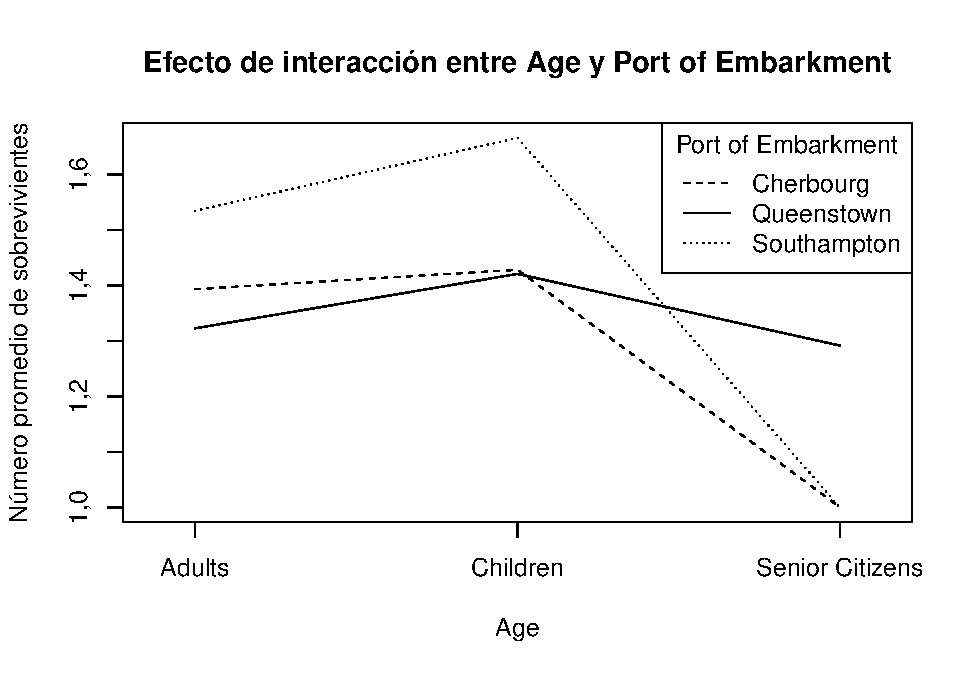
\includegraphics{titanicDataClean_files/figure-latex/unnamed-chunk-22-1.pdf}

\subsection{ANOVA}\label{anova}

Los principales efectos de Clase de Pasajero, Sexo y Puerto de Embarque
son significativos. Hubo más sobrevivientes en la primera clase en
comparación con la segunda y tercera clase. Hubo más mujeres
sobrevivientes. No hay un efecto significativo de la edad, lo que
significa que el número medio de supervivientes de todos los grupos de
edad fue casi el mismo.

\begin{Shaded}
\begin{Highlighting}[]
\NormalTok{me1 =}\StringTok{ }\KeywordTok{aov}\NormalTok{(df}\OperatorTok{$}\NormalTok{Survived }\OperatorTok{~}\StringTok{ }\NormalTok{df}\OperatorTok{$}\NormalTok{Pclass)}
\KeywordTok{anova}\NormalTok{(me1)}
\end{Highlighting}
\end{Shaded}

\begin{verbatim}
## Analysis of Variance Table
## 
## Response: df$Survived
##            Df  Sum Sq Mean Sq F value    Pr(>F)    
## df$Pclass   1  24,143 24,1429  115,03 < 2,2e-16 ***
## Residuals 889 186,584  0,2099                      
## ---
## Signif. codes:  0 '***' 0,001 '**' 0,01 '*' 0,05 '.' 0,1 ' ' 1
\end{verbatim}

\begin{Shaded}
\begin{Highlighting}[]
\NormalTok{me2 =}\StringTok{ }\KeywordTok{aov}\NormalTok{(df}\OperatorTok{$}\NormalTok{Survived }\OperatorTok{~}\StringTok{ }\NormalTok{df}\OperatorTok{$}\NormalTok{Sex)}
\KeywordTok{anova}\NormalTok{(me2)}
\end{Highlighting}
\end{Shaded}

\begin{verbatim}
## Analysis of Variance Table
## 
## Response: df$Survived
##            Df  Sum Sq Mean Sq F value    Pr(>F)    
## df$Sex      1  62,213  62,213  372,41 < 2,2e-16 ***
## Residuals 889 148,514   0,167                      
## ---
## Signif. codes:  0 '***' 0,001 '**' 0,01 '*' 0,05 '.' 0,1 ' ' 1
\end{verbatim}

\begin{Shaded}
\begin{Highlighting}[]
\NormalTok{me3 =}\StringTok{ }\KeywordTok{aov}\NormalTok{(df}\OperatorTok{$}\NormalTok{Survived }\OperatorTok{~}\StringTok{ }\NormalTok{df}\OperatorTok{$}\NormalTok{Age)}
\KeywordTok{anova}\NormalTok{(me3)}
\end{Highlighting}
\end{Shaded}

\begin{verbatim}
## Analysis of Variance Table
## 
## Response: df$Survived
##            Df  Sum Sq Mean Sq F value Pr(>F)
## df$Age      1   0,166 0,16606  0,7011 0,4026
## Residuals 889 210,561 0,23685
\end{verbatim}

\begin{Shaded}
\begin{Highlighting}[]
\NormalTok{me4 =}\StringTok{ }\KeywordTok{aov}\NormalTok{(df}\OperatorTok{$}\NormalTok{Survived }\OperatorTok{~}\StringTok{ }\NormalTok{df}\OperatorTok{$}\NormalTok{Embarked)}
\KeywordTok{anova}\NormalTok{(me4)}
\end{Highlighting}
\end{Shaded}

\begin{verbatim}
## Analysis of Variance Table
## 
## Response: df$Survived
##              Df  Sum Sq Mean Sq F value    Pr(>F)    
## df$Embarked   1   5,925  5,9246  25,717 4,811e-07 ***
## Residuals   889 204,803  0,2304                      
## ---
## Signif. codes:  0 '***' 0,001 '**' 0,01 '*' 0,05 '.' 0,1 ' ' 1
\end{verbatim}

Existen importantes efectos principales de Clase de Pasajero, Sexo y
Puerto de Embarque. Esto se ve reforzado una vez más por los ANOVA de
interacción bidireccional. Los efectos de interacción de la Clase de
Pasajeros son significativos con Sexo y Edad, pero no con Puerto de
Embarque. Los efectos de interacción del sexo no son significativos con
la edad o el puerto de embarque. El efecto de interacción de Age with
Port of Embarkment no es significativo.

\begin{Shaded}
\begin{Highlighting}[]
\NormalTok{ie12 =}\StringTok{ }\KeywordTok{aov}\NormalTok{(df}\OperatorTok{$}\NormalTok{Survived }\OperatorTok{~}\StringTok{ }\NormalTok{df}\OperatorTok{$}\NormalTok{Pclass }\OperatorTok{*}\StringTok{ }\NormalTok{df}\OperatorTok{$}\NormalTok{Sex)}
\KeywordTok{anova}\NormalTok{(ie12)}
\end{Highlighting}
\end{Shaded}

\begin{verbatim}
## Analysis of Variance Table
## 
## Response: df$Survived
##                   Df  Sum Sq Mean Sq F value    Pr(>F)    
## df$Pclass          1  24,143  24,143 164,061 < 2,2e-16 ***
## df$Sex             1  53,337  53,337 362,450 < 2,2e-16 ***
## df$Pclass:df$Sex   1   2,718   2,718  18,471 1,916e-05 ***
## Residuals        887 130,529   0,147                      
## ---
## Signif. codes:  0 '***' 0,001 '**' 0,01 '*' 0,05 '.' 0,1 ' ' 1
\end{verbatim}

\begin{Shaded}
\begin{Highlighting}[]
\NormalTok{ie13 =}\StringTok{ }\KeywordTok{aov}\NormalTok{(df}\OperatorTok{$}\NormalTok{Survived }\OperatorTok{~}\StringTok{ }\NormalTok{df}\OperatorTok{$}\NormalTok{Pclass }\OperatorTok{*}\StringTok{ }\NormalTok{df}\OperatorTok{$}\NormalTok{Age)}
\KeywordTok{anova}\NormalTok{(ie13)}
\end{Highlighting}
\end{Shaded}

\begin{verbatim}
## Analysis of Variance Table
## 
## Response: df$Survived
##                   Df  Sum Sq Mean Sq  F value    Pr(>F)    
## df$Pclass          1  24,143 24,1429 116,0401 < 2,2e-16 ***
## df$Age             1   0,439  0,4391   2,1104  0,146659    
## df$Pclass:df$Age   1   1,599  1,5991   7,6861  0,005681 ** 
## Residuals        887 184,546  0,2081                       
## ---
## Signif. codes:  0 '***' 0,001 '**' 0,01 '*' 0,05 '.' 0,1 ' ' 1
\end{verbatim}

\begin{Shaded}
\begin{Highlighting}[]
\NormalTok{ie14 =}\StringTok{ }\KeywordTok{aov}\NormalTok{(df}\OperatorTok{$}\NormalTok{Survived }\OperatorTok{~}\StringTok{ }\NormalTok{df}\OperatorTok{$}\NormalTok{Pclass }\OperatorTok{*}\StringTok{ }\NormalTok{df}\OperatorTok{$}\NormalTok{Embarked)}
\KeywordTok{anova}\NormalTok{(ie14)}
\end{Highlighting}
\end{Shaded}

\begin{verbatim}
## Analysis of Variance Table
## 
## Response: df$Survived
##                        Df  Sum Sq Mean Sq F value    Pr(>F)    
## df$Pclass               1  24,143 24,1429 116,817 < 2,2e-16 ***
## df$Embarked             1   2,754  2,7540  13,325 0,0002771 ***
## df$Pclass:df$Embarked   1   0,512  0,5115   2,475 0,1160273    
## Residuals             887 183,319  0,2067                      
## ---
## Signif. codes:  0 '***' 0,001 '**' 0,01 '*' 0,05 '.' 0,1 ' ' 1
\end{verbatim}

\begin{Shaded}
\begin{Highlighting}[]
\NormalTok{ie23 =}\StringTok{ }\KeywordTok{aov}\NormalTok{(df}\OperatorTok{$}\NormalTok{Survived }\OperatorTok{~}\StringTok{ }\NormalTok{df}\OperatorTok{$}\NormalTok{Sex }\OperatorTok{*}\StringTok{ }\NormalTok{df}\OperatorTok{$}\NormalTok{Age)}
\KeywordTok{anova}\NormalTok{(ie23)}
\end{Highlighting}
\end{Shaded}

\begin{verbatim}
## Analysis of Variance Table
## 
## Response: df$Survived
##                Df  Sum Sq Mean Sq  F value  Pr(>F)    
## df$Sex          1  62,213  62,213 373,1891 < 2e-16 ***
## df$Age          1   0,001   0,001   0,0044 0,94710    
## df$Sex:df$Age   1   0,644   0,644   3,8657 0,04959 *  
## Residuals     887 147,869   0,167                     
## ---
## Signif. codes:  0 '***' 0,001 '**' 0,01 '*' 0,05 '.' 0,1 ' ' 1
\end{verbatim}

\begin{Shaded}
\begin{Highlighting}[]
\NormalTok{ie24 =}\StringTok{ }\KeywordTok{aov}\NormalTok{(df}\OperatorTok{$}\NormalTok{Survived }\OperatorTok{~}\StringTok{ }\NormalTok{df}\OperatorTok{$}\NormalTok{Sex }\OperatorTok{*}\StringTok{ }\NormalTok{df}\OperatorTok{$}\NormalTok{Embarked)}
\KeywordTok{anova}\NormalTok{(ie24)}
\end{Highlighting}
\end{Shaded}

\begin{verbatim}
## Analysis of Variance Table
## 
## Response: df$Survived
##                     Df  Sum Sq Mean Sq  F value    Pr(>F)    
## df$Sex               1  62,213  62,213 378,4640 < 2,2e-16 ***
## df$Embarked          1   2,526   2,526  15,3691 9,524e-05 ***
## df$Sex:df$Embarked   1   0,180   0,180   1,0932    0,2961    
## Residuals          887 145,808   0,164                       
## ---
## Signif. codes:  0 '***' 0,001 '**' 0,01 '*' 0,05 '.' 0,1 ' ' 1
\end{verbatim}

\begin{Shaded}
\begin{Highlighting}[]
\NormalTok{ie34 =}\StringTok{ }\KeywordTok{aov}\NormalTok{(df}\OperatorTok{$}\NormalTok{Survived }\OperatorTok{~}\StringTok{ }\NormalTok{df}\OperatorTok{$}\NormalTok{Age }\OperatorTok{*}\StringTok{ }\NormalTok{df}\OperatorTok{$}\NormalTok{Embarked)}
\KeywordTok{anova}\NormalTok{(ie34)}
\end{Highlighting}
\end{Shaded}

\begin{verbatim}
## Analysis of Variance Table
## 
## Response: df$Survived
##                     Df  Sum Sq Mean Sq F value    Pr(>F)    
## df$Age               1   0,166  0,1661  0,7204    0,3963    
## df$Embarked          1   5,869  5,8694 25,4604 5,478e-07 ***
## df$Age:df$Embarked   1   0,212  0,2116  0,9180    0,3383    
## Residuals          887 204,480  0,2305                      
## ---
## Signif. codes:  0 '***' 0,001 '**' 0,01 '*' 0,05 '.' 0,1 ' ' 1
\end{verbatim}

\subsubsection{Estimacion}\label{estimacion}

En base al análisis de datos exploratorios, efectos principales, efectos
de interacción bidireccional y ANOVA para todos los efectos principales
y de interacción, podemos estimar que si el buque del Titanic volviera a
zarpar (para el caso, cualquier barco) y si fuera para terminar con el
mismo destino, entonces, en promedio, habría más sobrevivientes de la
clase alta, más sobrevivientes que son mujeres y niños y más
sobrevivientes que abordaron el barco en Cherbourg.

\subsubsection{Diagnóstico y verificación de adecuación del
modelo}\label{diagnostico-y-verificacion-de-adecuacion-del-modelo}

El diagrama Q-Q es una herramienta para comparar dos distribuciones
entre sí en base a la comparación de sus cuantiles. Ninguno de los
gráficos de Q-Q a continuación se adhieren a la línea, lo que significa
que los datos son de naturaleza altamente no lineal. Además, la no
linealidad de los puntos sugiere que los datos no se distribuyen
normalmente.

El gráfico residual se utiliza en el análisis de datos estadísticos para
detectar la no linealidad de los datos, varianzas de errores desiguales
y valores atípicos. En la mayoría de las siguientes parcelas residuales
vs fit, los residuos no rebotan aleatoriamente alrededor de la línea
cero, pero parecen ajustarse a una línea que tiene una pendiente
negativa. Esto sugiere que los datos no son de naturaleza lineal. Los
residuos forman aproximadamente una banda horizontal alrededor de la
línea cero, lo que sugiere que las varianzas de los términos de error
son iguales. Por último, no hay residuos que se destaquen del patrón
básico de los residuos, lo que sugiere que no hay valores atípicos.

Estas observaciones sugieren que el conjunto de datos no ha cumplido
todas las suposiciones para implementar ANOVA. Y esto es cierto porque,
como se explicó anteriormente, no hubo alcance de replicación y medidas
repetidas. Sin embargo, aún obtenemos resultados razonables porque hubo
algunas suposiciones para ANOVA que eran verdaderas en el conjunto de
datos.

\begin{Shaded}
\begin{Highlighting}[]
\KeywordTok{qqnorm}\NormalTok{(}\KeywordTok{residuals}\NormalTok{(me1))}
\KeywordTok{qqline}\NormalTok{(}\KeywordTok{residuals}\NormalTok{(me1))}
\end{Highlighting}
\end{Shaded}

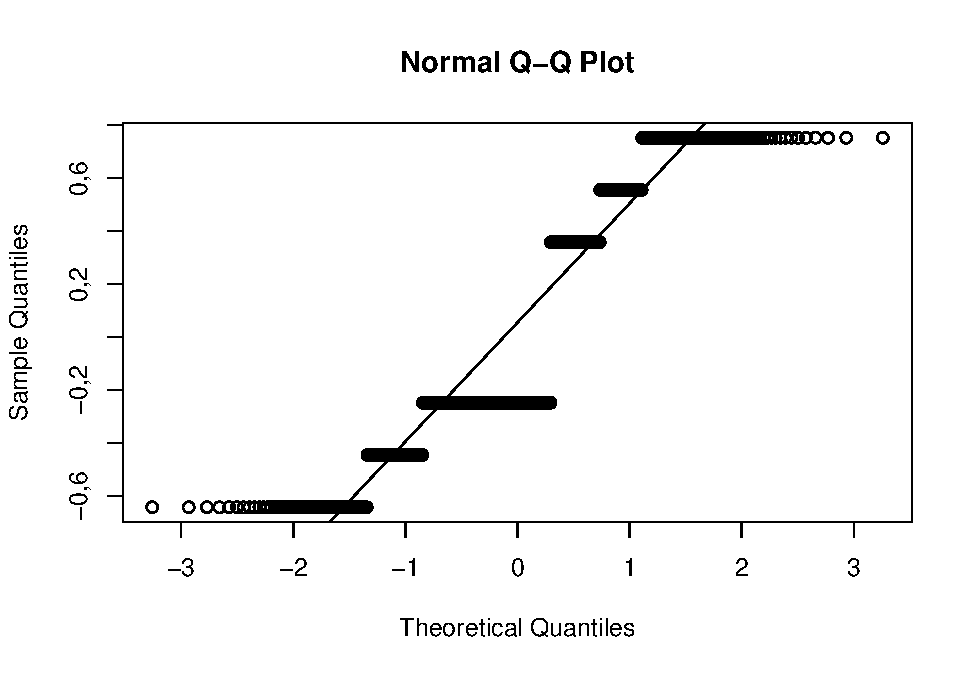
\includegraphics{titanicDataClean_files/figure-latex/unnamed-chunk-25-1.pdf}

\begin{Shaded}
\begin{Highlighting}[]
\KeywordTok{plot}\NormalTok{(}\KeywordTok{fitted}\NormalTok{(me1), }\KeywordTok{residuals}\NormalTok{(me1))}
\end{Highlighting}
\end{Shaded}

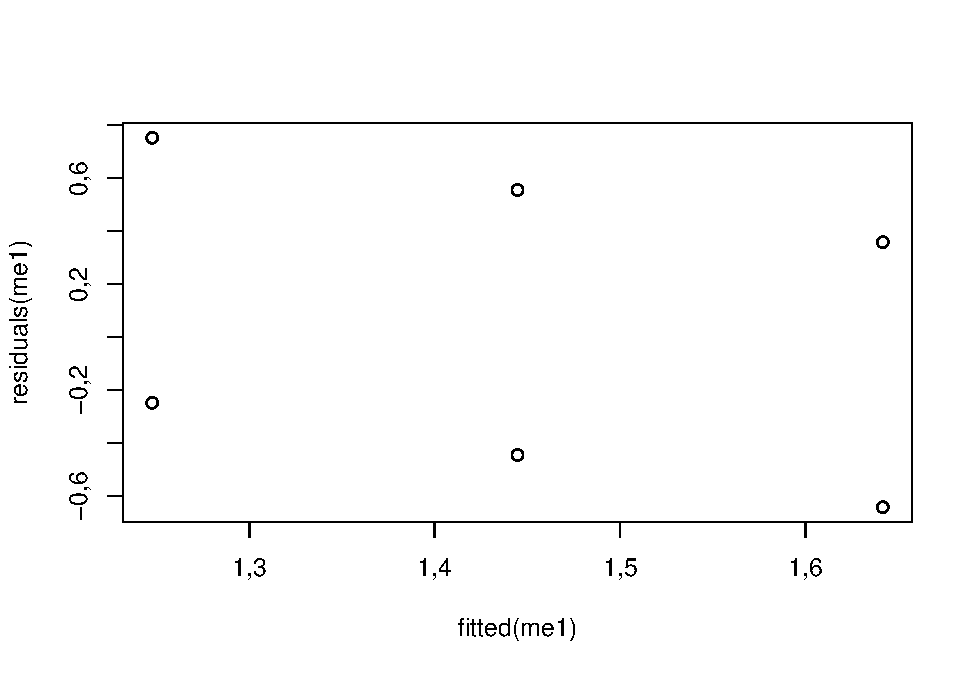
\includegraphics{titanicDataClean_files/figure-latex/unnamed-chunk-25-2.pdf}

\begin{Shaded}
\begin{Highlighting}[]
\KeywordTok{qqnorm}\NormalTok{(}\KeywordTok{residuals}\NormalTok{(me2))}
\KeywordTok{qqline}\NormalTok{(}\KeywordTok{residuals}\NormalTok{(me2))}
\end{Highlighting}
\end{Shaded}

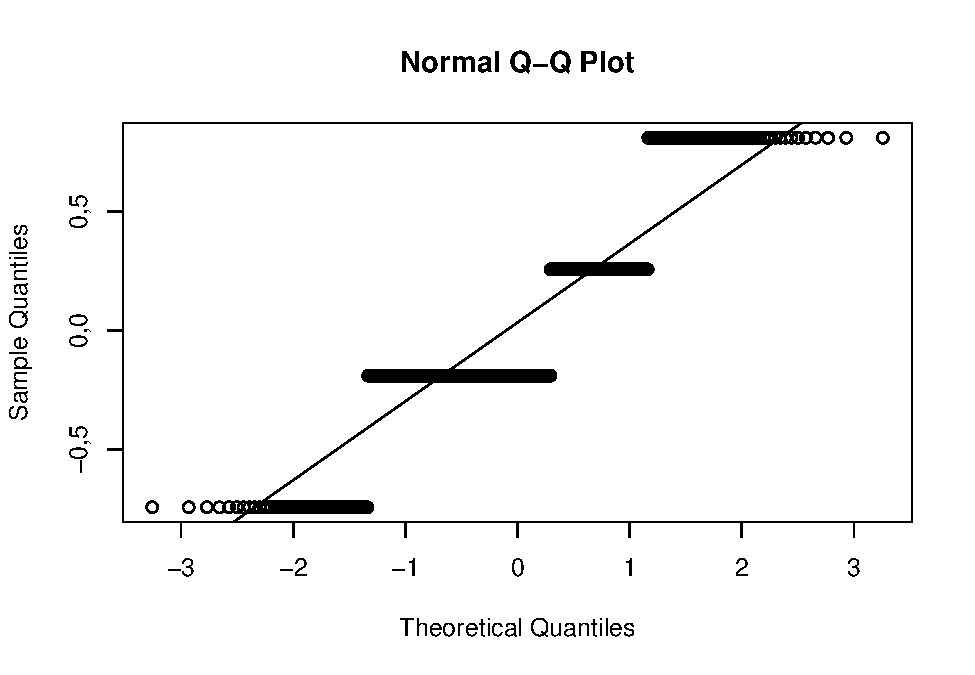
\includegraphics{titanicDataClean_files/figure-latex/unnamed-chunk-25-3.pdf}

\begin{Shaded}
\begin{Highlighting}[]
\KeywordTok{plot}\NormalTok{(}\KeywordTok{fitted}\NormalTok{(me2), }\KeywordTok{residuals}\NormalTok{(me2))}
\end{Highlighting}
\end{Shaded}

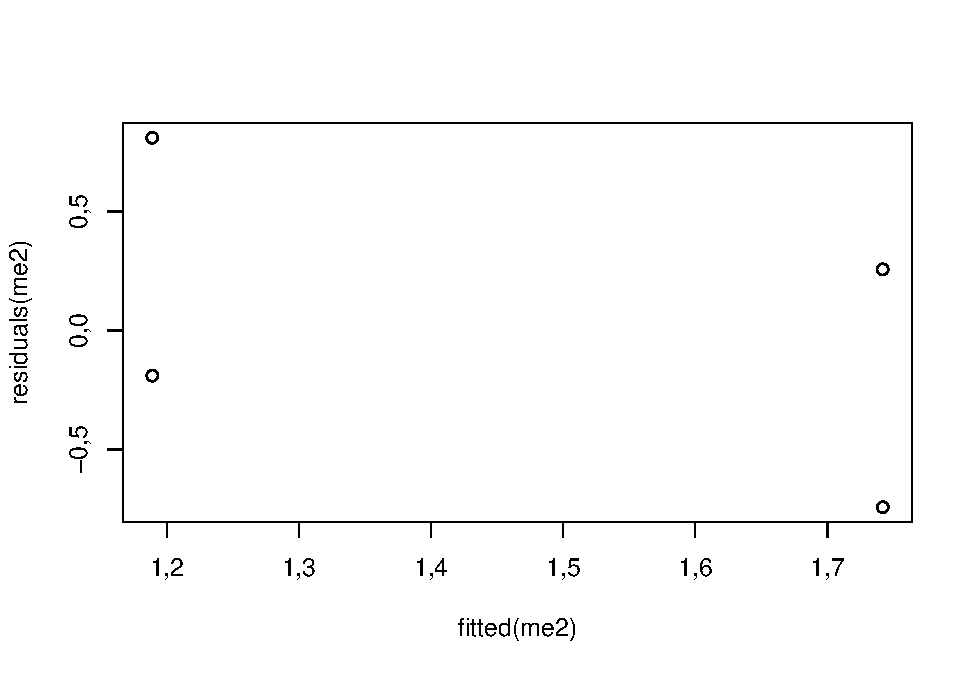
\includegraphics{titanicDataClean_files/figure-latex/unnamed-chunk-25-4.pdf}

\begin{Shaded}
\begin{Highlighting}[]
\KeywordTok{qqnorm}\NormalTok{(}\KeywordTok{residuals}\NormalTok{(me3))}
\KeywordTok{qqline}\NormalTok{(}\KeywordTok{residuals}\NormalTok{(me3))}
\end{Highlighting}
\end{Shaded}

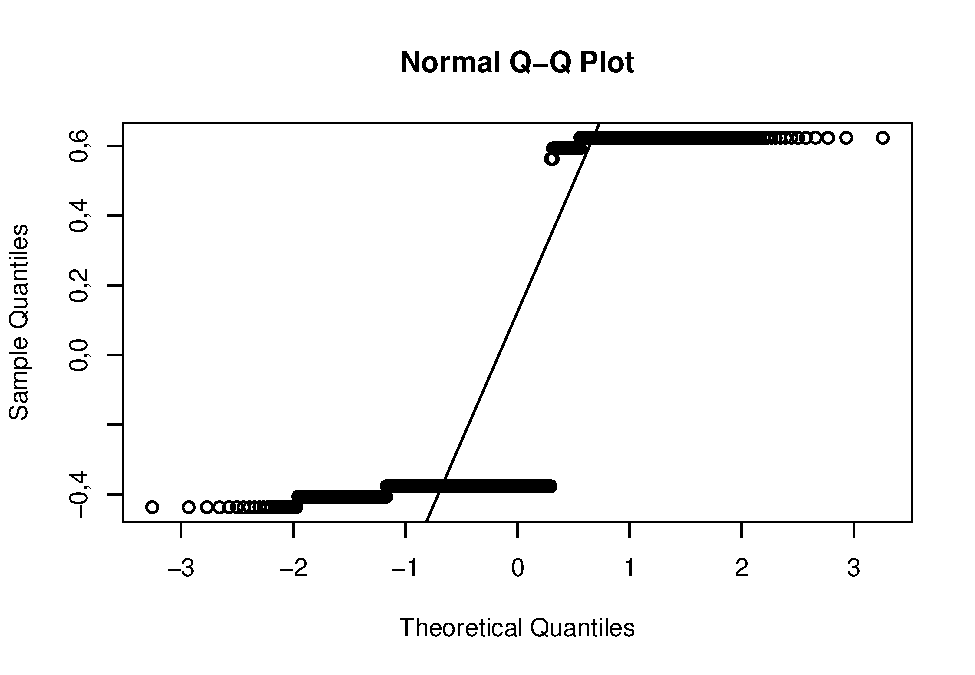
\includegraphics{titanicDataClean_files/figure-latex/unnamed-chunk-25-5.pdf}

\begin{Shaded}
\begin{Highlighting}[]
\KeywordTok{plot}\NormalTok{(}\KeywordTok{fitted}\NormalTok{(me3), }\KeywordTok{residuals}\NormalTok{(me3))}
\end{Highlighting}
\end{Shaded}

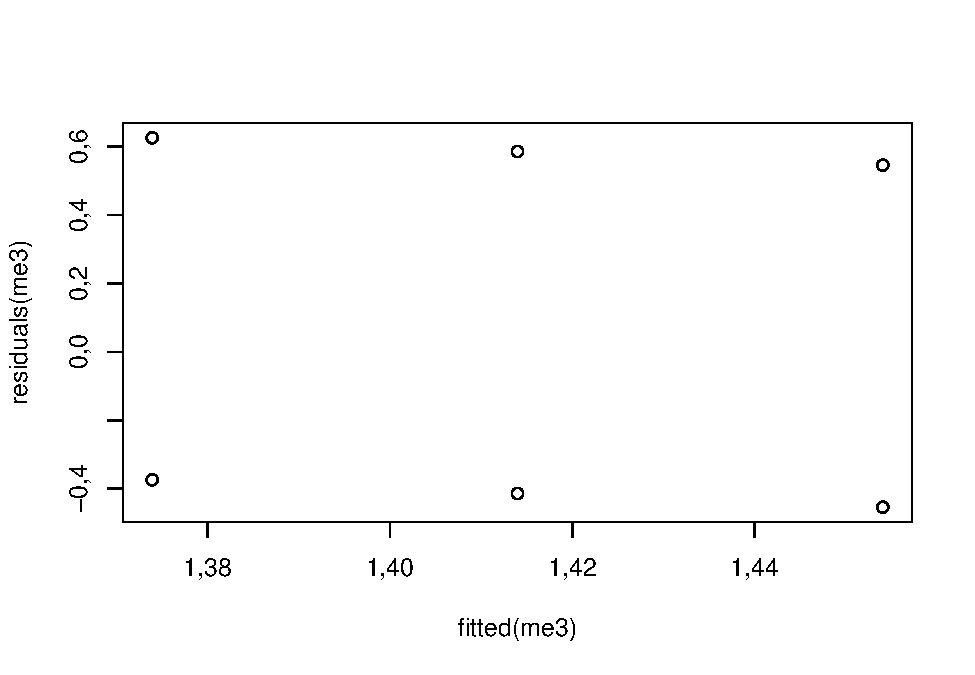
\includegraphics{titanicDataClean_files/figure-latex/unnamed-chunk-25-6.pdf}

\begin{Shaded}
\begin{Highlighting}[]
\KeywordTok{qqnorm}\NormalTok{(}\KeywordTok{residuals}\NormalTok{(me4))}
\KeywordTok{qqline}\NormalTok{(}\KeywordTok{residuals}\NormalTok{(me4))}
\end{Highlighting}
\end{Shaded}

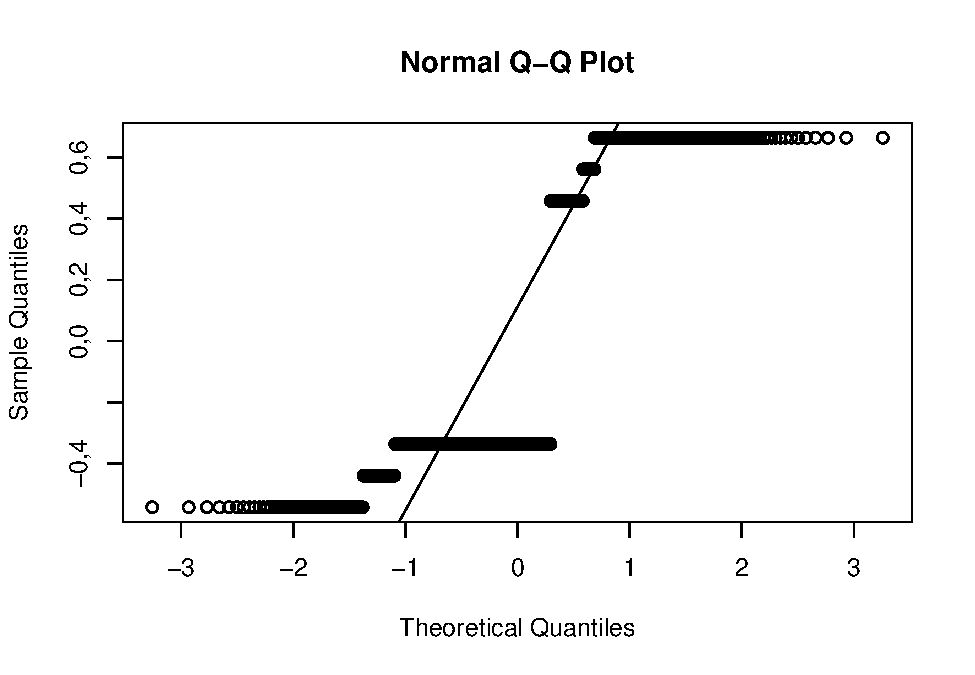
\includegraphics{titanicDataClean_files/figure-latex/unnamed-chunk-25-7.pdf}

\begin{Shaded}
\begin{Highlighting}[]
\KeywordTok{plot}\NormalTok{(}\KeywordTok{fitted}\NormalTok{(me4), }\KeywordTok{residuals}\NormalTok{(me4))}
\end{Highlighting}
\end{Shaded}

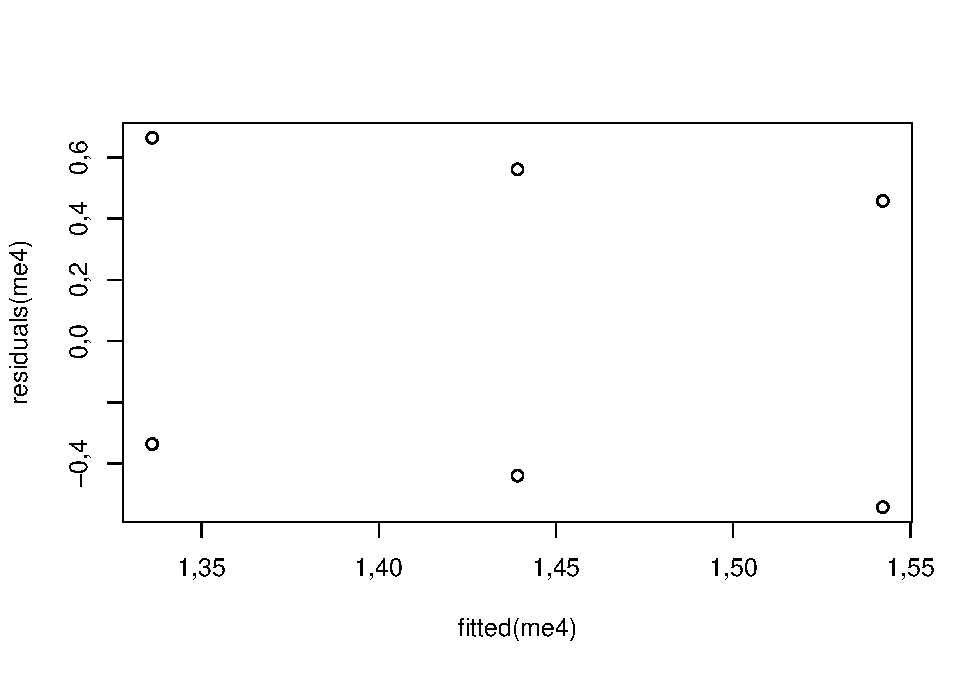
\includegraphics{titanicDataClean_files/figure-latex/unnamed-chunk-25-8.pdf}

\begin{Shaded}
\begin{Highlighting}[]
\KeywordTok{qqnorm}\NormalTok{(}\KeywordTok{residuals}\NormalTok{(ie12))}
\KeywordTok{qqline}\NormalTok{(}\KeywordTok{residuals}\NormalTok{(ie12))}
\end{Highlighting}
\end{Shaded}

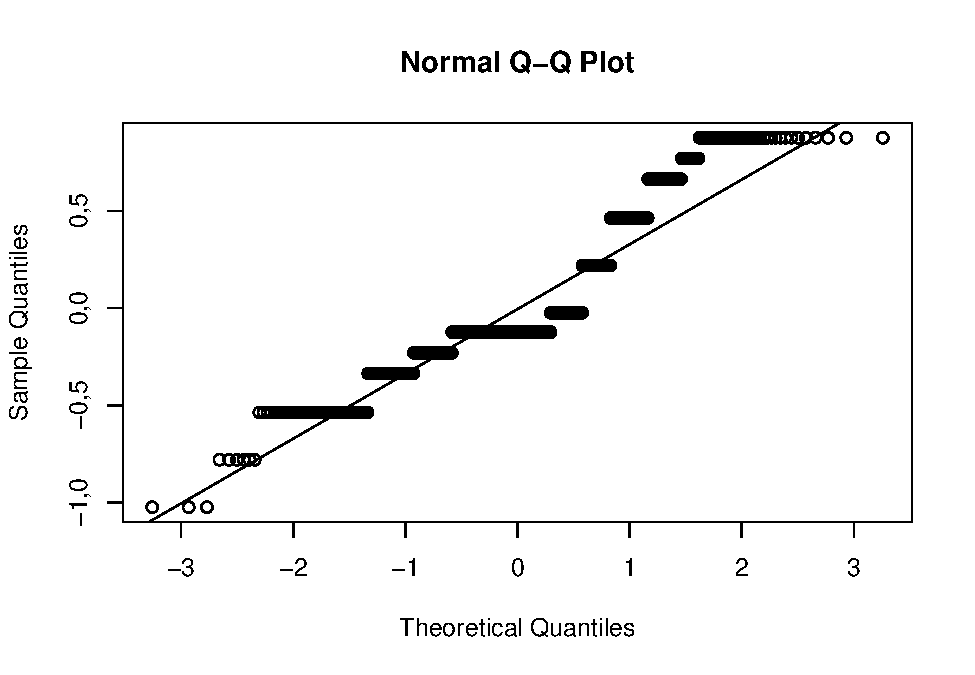
\includegraphics{titanicDataClean_files/figure-latex/unnamed-chunk-25-9.pdf}

\begin{Shaded}
\begin{Highlighting}[]
\KeywordTok{plot}\NormalTok{(}\KeywordTok{fitted}\NormalTok{(ie12), }\KeywordTok{residuals}\NormalTok{(ie12))}
\end{Highlighting}
\end{Shaded}

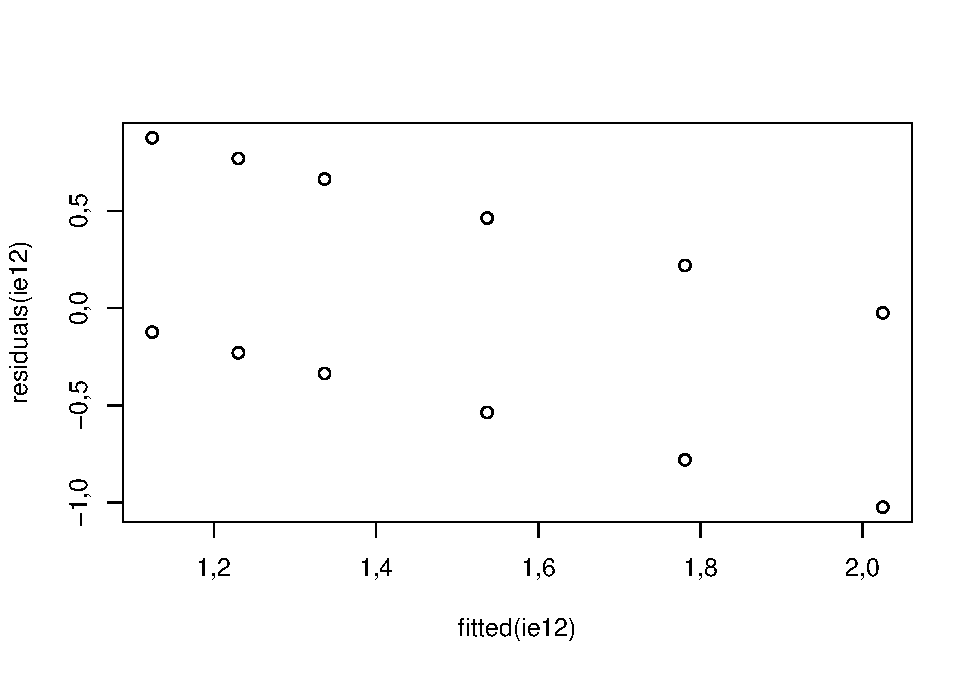
\includegraphics{titanicDataClean_files/figure-latex/unnamed-chunk-25-10.pdf}

\begin{Shaded}
\begin{Highlighting}[]
\KeywordTok{qqnorm}\NormalTok{(}\KeywordTok{residuals}\NormalTok{(ie13))}
\KeywordTok{qqline}\NormalTok{(}\KeywordTok{residuals}\NormalTok{(ie13))}
\end{Highlighting}
\end{Shaded}

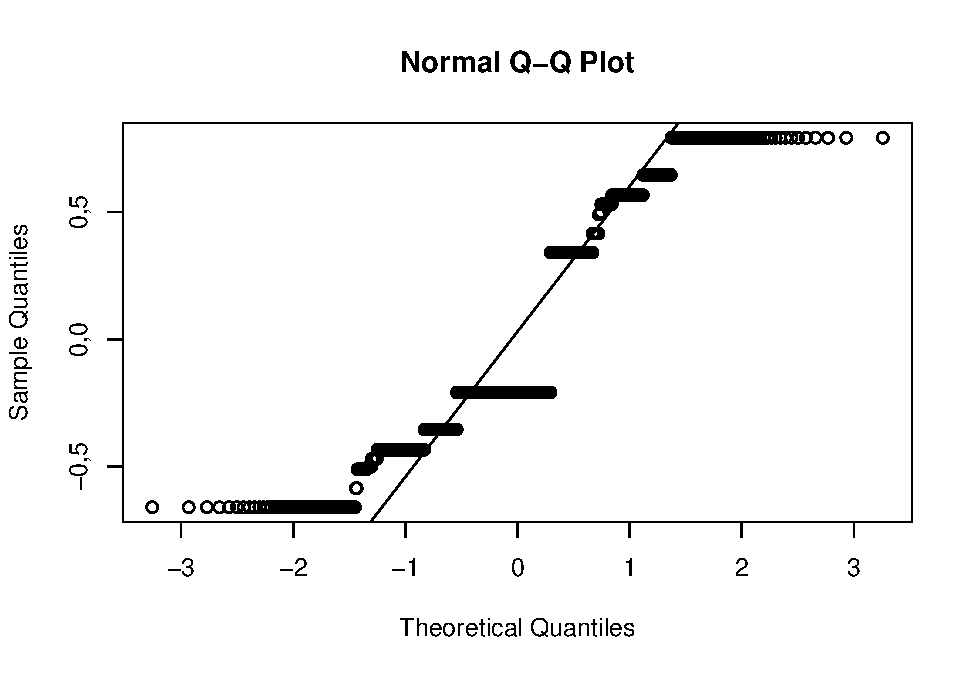
\includegraphics{titanicDataClean_files/figure-latex/unnamed-chunk-25-11.pdf}

\begin{Shaded}
\begin{Highlighting}[]
\KeywordTok{plot}\NormalTok{(}\KeywordTok{fitted}\NormalTok{(ie13), }\KeywordTok{residuals}\NormalTok{(ie13))}
\end{Highlighting}
\end{Shaded}

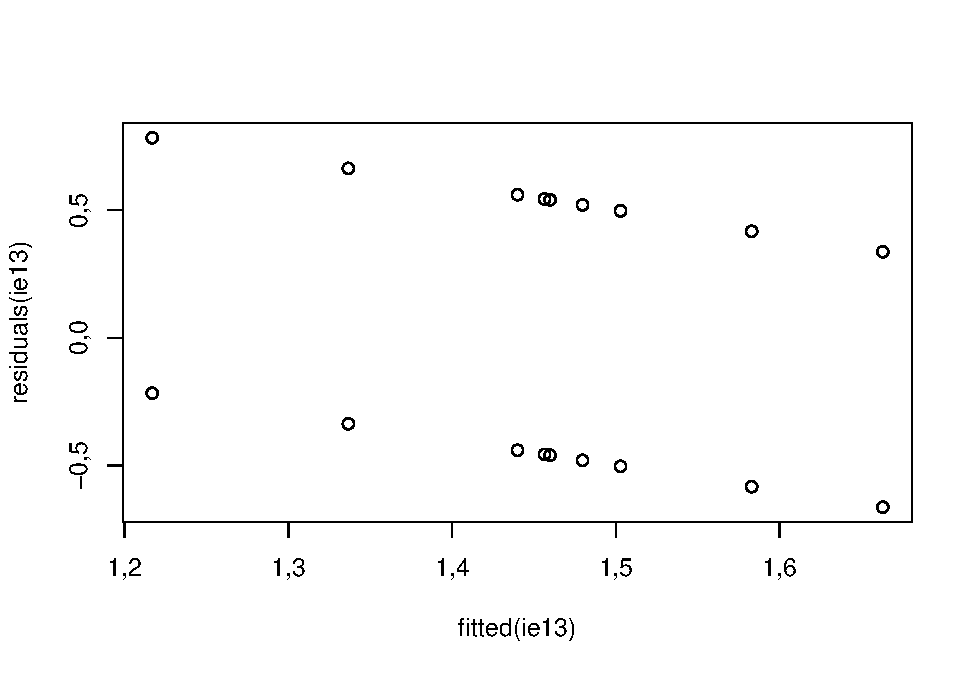
\includegraphics{titanicDataClean_files/figure-latex/unnamed-chunk-25-12.pdf}

\begin{Shaded}
\begin{Highlighting}[]
\KeywordTok{qqnorm}\NormalTok{(}\KeywordTok{residuals}\NormalTok{(ie14))}
\KeywordTok{qqline}\NormalTok{(}\KeywordTok{residuals}\NormalTok{(ie14))}
\end{Highlighting}
\end{Shaded}

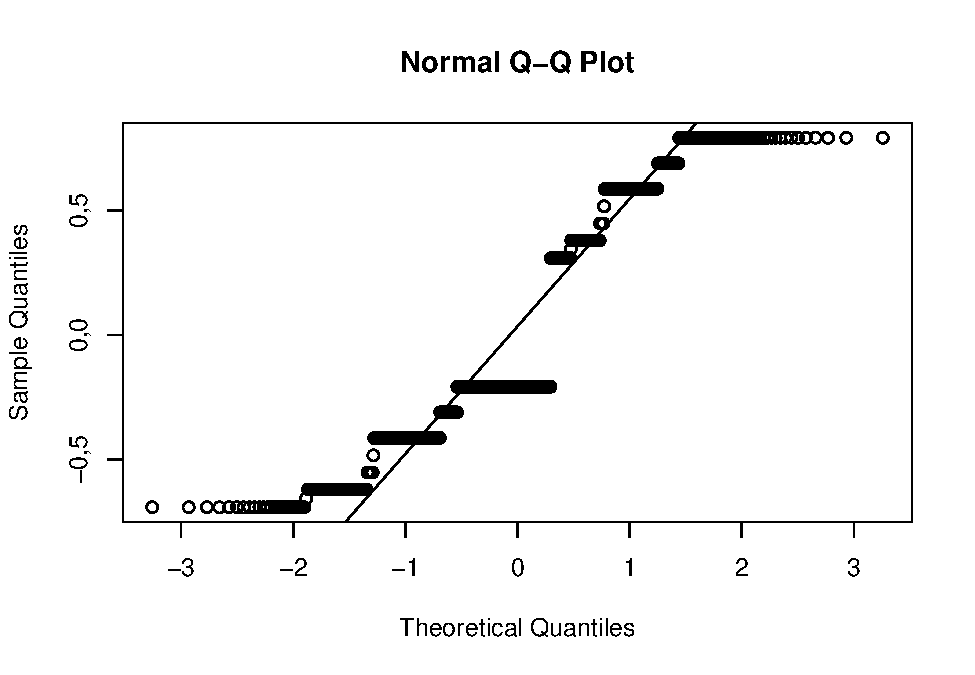
\includegraphics{titanicDataClean_files/figure-latex/unnamed-chunk-25-13.pdf}

\begin{Shaded}
\begin{Highlighting}[]
\KeywordTok{plot}\NormalTok{(}\KeywordTok{fitted}\NormalTok{(ie14), }\KeywordTok{residuals}\NormalTok{(ie14))}
\end{Highlighting}
\end{Shaded}

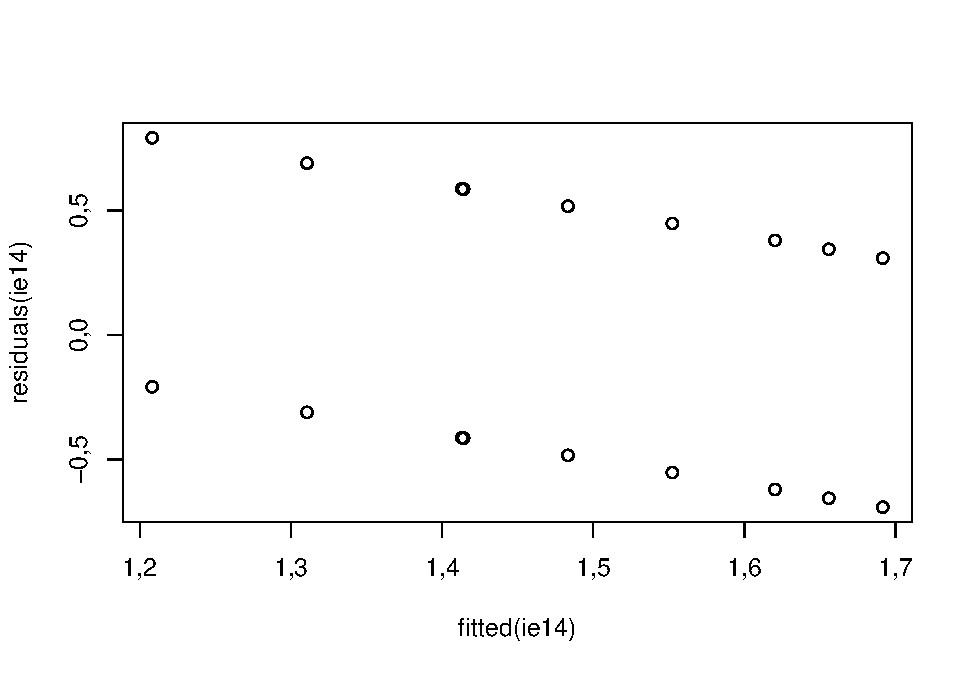
\includegraphics{titanicDataClean_files/figure-latex/unnamed-chunk-25-14.pdf}

\begin{Shaded}
\begin{Highlighting}[]
\KeywordTok{qqnorm}\NormalTok{(}\KeywordTok{residuals}\NormalTok{(ie23))}
\KeywordTok{qqline}\NormalTok{(}\KeywordTok{residuals}\NormalTok{(ie23))}
\end{Highlighting}
\end{Shaded}

\includegraphics{titanicDataClean_files/figure-latex/unnamed-chunk-25-15.pdf}

\begin{Shaded}
\begin{Highlighting}[]
\KeywordTok{plot}\NormalTok{(}\KeywordTok{fitted}\NormalTok{(ie23), }\KeywordTok{residuals}\NormalTok{(ie23))}
\end{Highlighting}
\end{Shaded}

\includegraphics{titanicDataClean_files/figure-latex/unnamed-chunk-25-16.pdf}

\begin{Shaded}
\begin{Highlighting}[]
\KeywordTok{qqnorm}\NormalTok{(}\KeywordTok{residuals}\NormalTok{(ie24))}
\KeywordTok{qqline}\NormalTok{(}\KeywordTok{residuals}\NormalTok{(ie24))}
\end{Highlighting}
\end{Shaded}

\includegraphics{titanicDataClean_files/figure-latex/unnamed-chunk-25-17.pdf}

\begin{Shaded}
\begin{Highlighting}[]
\KeywordTok{plot}\NormalTok{(}\KeywordTok{fitted}\NormalTok{(ie24), }\KeywordTok{residuals}\NormalTok{(ie24))}
\end{Highlighting}
\end{Shaded}

\includegraphics{titanicDataClean_files/figure-latex/unnamed-chunk-25-18.pdf}

\begin{Shaded}
\begin{Highlighting}[]
\KeywordTok{qqnorm}\NormalTok{(}\KeywordTok{residuals}\NormalTok{(ie34))}
\KeywordTok{qqline}\NormalTok{(}\KeywordTok{residuals}\NormalTok{(ie34))}
\end{Highlighting}
\end{Shaded}

\includegraphics{titanicDataClean_files/figure-latex/unnamed-chunk-25-19.pdf}

\begin{Shaded}
\begin{Highlighting}[]
\KeywordTok{plot}\NormalTok{(}\KeywordTok{fitted}\NormalTok{(ie34), }\KeywordTok{residuals}\NormalTok{(ie34))}
\end{Highlighting}
\end{Shaded}

\includegraphics{titanicDataClean_files/figure-latex/unnamed-chunk-25-20.pdf}

\subsection{Evaluación de algoritmos}\label{evaluacion-de-algoritmos}

Intentaremos algunos algoritmos lineales y no lineales: * Algoritmos
Lineales: Regresión Logística (LG), Análisis Lineal Discriminado (LDA) y
Regresión Logística Regularizada (GLMNET). * Algoritmos no lineales:
k-Nearest Neighbors (KNN), árboles de clasificación y regresión (CART),
Naive Bayes (NB) y máquinas de vectores de soporte con funciones de base
radial (SVM).

\subsubsection{Selección y verificación de
variables}\label{seleccion-y-verificacion-de-variables}

A partir de los valores de muestra que se muestran en el conjunto de
datos, podemos ver que PassengerId, Name, Ticket, Cabin y Embarked
probablemente no serán útiles en nuestro análisis, por lo que decidimos
que podemos eliminar estas variables.

\begin{Shaded}
\begin{Highlighting}[]
\CommentTok{# se eliminan variables redundantes}
\NormalTok{datasetTrain <-}\StringTok{ }\NormalTok{titanic_train[,}\KeywordTok{c}\NormalTok{(}\OperatorTok{-}\DecValTok{3}\NormalTok{, }\OperatorTok{-}\DecValTok{8}\NormalTok{, }\OperatorTok{-}\DecValTok{10}\NormalTok{, }\OperatorTok{-}\DecValTok{11}\NormalTok{, }\OperatorTok{-}\KeywordTok{c}\NormalTok{(}\DecValTok{12}\OperatorTok{:}\DecValTok{23}\NormalTok{))]}

\NormalTok{datasetTrain}\OperatorTok{$}\NormalTok{Pclass =}\StringTok{ }\KeywordTok{as.integer}\NormalTok{(datasetTrain}\OperatorTok{$}\NormalTok{Pclass)}
\NormalTok{datasetTrain}\OperatorTok{$}\NormalTok{Age =}\StringTok{ }\KeywordTok{as.integer}\NormalTok{(datasetTrain}\OperatorTok{$}\NormalTok{Age)}
\CommentTok{#datasetTrain$Survived = as.integer(datasetTrain$Survived)}
\CommentTok{# sumario}
\KeywordTok{summary}\NormalTok{(datasetTrain)}
\end{Highlighting}
\end{Shaded}

\begin{verbatim}
##  Survived     Pclass          Sex           Age            SibSp      
##  0:549    Min.   :1,000   female:314   Min.   : 0,00   Min.   :0,000  
##  1:342    1st Qu.:2,000   male  :577   1st Qu.:20,00   1st Qu.:0,000  
##           Median :3,000                Median :28,00   Median :0,000  
##           Mean   :2,309                Mean   :29,39   Mean   :0,523  
##           3rd Qu.:3,000                3rd Qu.:38,00   3rd Qu.:1,000  
##           Max.   :3,000                Max.   :80,00   Max.   :8,000  
##      Parch             Fare       
##  Min.   :0,0000   Min.   :  0,00  
##  1st Qu.:0,0000   1st Qu.:  7,91  
##  Median :0,0000   Median : 14,45  
##  Mean   :0,3816   Mean   : 32,20  
##  3rd Qu.:0,0000   3rd Qu.: 31,00  
##  Max.   :6,0000   Max.   :512,33
\end{verbatim}

\begin{Shaded}
\begin{Highlighting}[]
\KeywordTok{sapply}\NormalTok{(datasetTrain, class)}
\end{Highlighting}
\end{Shaded}

\begin{verbatim}
##  Survived    Pclass       Sex       Age     SibSp     Parch      Fare 
##  "factor" "integer"  "factor" "integer" "integer" "integer" "numeric"
\end{verbatim}

Echemos un vistazo más de cerca a las distribuciones de clase.

\begin{Shaded}
\begin{Highlighting}[]
\CommentTok{# distribución de clases}
\KeywordTok{cbind}\NormalTok{(}\DataTypeTok{freq=}\KeywordTok{table}\NormalTok{(datasetTrain}\OperatorTok{$}\NormalTok{Survived), }\DataTypeTok{percentage=}\KeywordTok{prop.table}\NormalTok{(}\KeywordTok{table}\NormalTok{(datasetTrain}\OperatorTok{$}\NormalTok{Survived))}\OperatorTok{*}\DecValTok{100}\NormalTok{)}
\end{Highlighting}
\end{Shaded}

\begin{verbatim}
##   freq percentage
## 0  549   61,61616
## 1  342   38,38384
\end{verbatim}

Hay algún desequilibrio en los valores de la clase. Observamos una
división aproximada de 60\% a 40\% para Died (= 0) y Survived (= 1) en
los valores de clase.

\begin{Shaded}
\begin{Highlighting}[]
\NormalTok{datasetTrain[,}\DecValTok{3}\NormalTok{] <-}\StringTok{ }\KeywordTok{as.numeric}\NormalTok{((datasetTrain[,}\DecValTok{3}\NormalTok{]))}
\NormalTok{complete_cases <-}\StringTok{ }\KeywordTok{complete.cases}\NormalTok{(datasetTrain)}

\KeywordTok{kable}\NormalTok{(}\KeywordTok{cor}\NormalTok{(datasetTrain[complete_cases,}\DecValTok{2}\OperatorTok{:}\DecValTok{5}\NormalTok{]), }\DataTypeTok{caption =} \StringTok{"Correlación del conjunto de datos"}\NormalTok{,}\DataTypeTok{digits =} \DecValTok{3}\NormalTok{, }\DataTypeTok{padding =} \DecValTok{2}\NormalTok{, }\DataTypeTok{align =} \StringTok{'r'}\NormalTok{)}
\end{Highlighting}
\end{Shaded}

\begin{longtable}[]{@{}lrrrr@{}}
\caption{Correlación del conjunto de datos}\tabularnewline
\toprule
& Pclass & Sex & Age & SibSp\tabularnewline
\midrule
\endfirsthead
\toprule
& Pclass & Sex & Age & SibSp\tabularnewline
\midrule
\endhead
Pclass & 1,000 & 0,132 & -0,369 & 0,083\tabularnewline
Sex & 0,132 & 1,000 & 0,072 & -0,115\tabularnewline
Age & -0,369 & 0,072 & 1,000 & -0,311\tabularnewline
SibSp & 0,083 & -0,115 & -0,311 & 1,000\tabularnewline
\bottomrule
\end{longtable}

\begin{Shaded}
\begin{Highlighting}[]
\CommentTok{#cor(datasetTrain[complete_cases,2:5])}
\end{Highlighting}
\end{Shaded}

Los valores por encima de 0,75 o por debajo de -0,75 son indicativos de
una correlación alta positiva o alta negativa. A partir de los
resultados anteriores, las variables no están altamente correlacionadas
en este conjunto de datos.

\subsubsection{Visualizacion del conjunto de
datos}\label{visualizacion-del-conjunto-de-datos}

\begin{Shaded}
\begin{Highlighting}[]
\CommentTok{# barra de hombres y mujeres que sobrevivieron}
\KeywordTok{barplot}\NormalTok{(}\KeywordTok{table}\NormalTok{(datasetTrain}\OperatorTok{$}\NormalTok{Survived, datasetTrain[,}\DecValTok{3}\NormalTok{]))}
\KeywordTok{legend}\NormalTok{(}\StringTok{"topleft"}\NormalTok{, }\DataTypeTok{legend =} \KeywordTok{c}\NormalTok{(}\StringTok{"Mueren"}\NormalTok{, }\StringTok{"Sobreviven"}\NormalTok{), }\DataTypeTok{fill=}\KeywordTok{c}\NormalTok{(}\StringTok{"black"}\NormalTok{,}\StringTok{"grey"}\NormalTok{))}
\end{Highlighting}
\end{Shaded}

\includegraphics{titanicDataClean_files/figure-latex/datasetTrain_plot_01-1.pdf}

\subsubsection{Opciones de prueba y métrica de
evaluación.}\label{opciones-de-prueba-y-metrica-de-evaluacion.}

Vamos a definir un test de control. Usaremos una validación cruzada de
10 veces con 3 repeticiones. Esta es una buena configuración de test de
control estándar. Es un problema de clasificación binario. Para
simplificar, utilizaremos métricas de precisión y Kappa.

\begin{verbatim}
FALSE corrplot 0.84 loaded
\end{verbatim}

\begin{Shaded}
\begin{Highlighting}[]
\CommentTok{# 10-fold validación cruzada con 3 repeticiones}
\NormalTok{trainControl <-}\StringTok{ }\KeywordTok{trainControl}\NormalTok{(}\DataTypeTok{method=}\StringTok{"repeatedcv"}\NormalTok{, }\DataTypeTok{number=}\DecValTok{10}\NormalTok{, }\DataTypeTok{repeats=}\DecValTok{3}\NormalTok{)}
\NormalTok{metric <-}\StringTok{ "Accuracy"}
\end{Highlighting}
\end{Shaded}

\subsubsection{Algoritmos de muestreo (Spot-Check
Algorithms)}\label{algoritmos-de-muestreo-spot-check-algorithms}

\begin{Shaded}
\begin{Highlighting}[]
\CommentTok{# LG}
\KeywordTok{set.seed}\NormalTok{(}\DecValTok{7}\NormalTok{)}
\NormalTok{fit.glm <-}\StringTok{ }\KeywordTok{train}\NormalTok{(Survived}\OperatorTok{~}\NormalTok{., }\DataTypeTok{data=}\NormalTok{datasetTrain, }\DataTypeTok{method=}\StringTok{"glm"}\NormalTok{, }\DataTypeTok{metric=}\NormalTok{metric, }
                 \DataTypeTok{trControl=}\NormalTok{trainControl)}

\CommentTok{# LDA}
\KeywordTok{set.seed}\NormalTok{(}\DecValTok{7}\NormalTok{)}
\NormalTok{fit.lda <-}\StringTok{ }\KeywordTok{train}\NormalTok{(Survived}\OperatorTok{~}\NormalTok{., }\DataTypeTok{data=}\NormalTok{datasetTrain, }\DataTypeTok{method=}\StringTok{"lda"}\NormalTok{, }\DataTypeTok{metric=}\NormalTok{metric, }
                 \DataTypeTok{trControl=}\NormalTok{trainControl)}

\CommentTok{# GLMNET}
\KeywordTok{set.seed}\NormalTok{(}\DecValTok{7}\NormalTok{)}
\NormalTok{fit.glmnet <-}\StringTok{ }\KeywordTok{train}\NormalTok{(Survived}\OperatorTok{~}\NormalTok{., }\DataTypeTok{data=}\NormalTok{datasetTrain, }\DataTypeTok{method=}\StringTok{"glmnet"}\NormalTok{, }\DataTypeTok{metric=}\NormalTok{metric,}
                    \DataTypeTok{trControl=}\NormalTok{trainControl)}

\CommentTok{# KNN}
\KeywordTok{set.seed}\NormalTok{(}\DecValTok{7}\NormalTok{)}
\NormalTok{fit.knn <-}\StringTok{ }\KeywordTok{train}\NormalTok{(Survived}\OperatorTok{~}\NormalTok{., }\DataTypeTok{data=}\NormalTok{datasetTrain, }\DataTypeTok{method=}\StringTok{"knn"}\NormalTok{, }\DataTypeTok{metric=}\NormalTok{metric, }
                 \DataTypeTok{trControl=}\NormalTok{trainControl)}

\CommentTok{# CART}
\KeywordTok{set.seed}\NormalTok{(}\DecValTok{7}\NormalTok{)}
\NormalTok{fit.cart <-}\StringTok{ }\KeywordTok{train}\NormalTok{(Survived}\OperatorTok{~}\NormalTok{., }\DataTypeTok{data=}\NormalTok{datasetTrain, }\DataTypeTok{method=}\StringTok{"rpart"}\NormalTok{, }\DataTypeTok{metric=}\NormalTok{metric,}
                  \DataTypeTok{trControl=}\NormalTok{trainControl)}

\CommentTok{# Naive Bayes}
\KeywordTok{set.seed}\NormalTok{(}\DecValTok{7}\NormalTok{)}
\NormalTok{fit.nb <-}\StringTok{ }\KeywordTok{train}\NormalTok{(Survived}\OperatorTok{~}\NormalTok{., }\DataTypeTok{data=}\NormalTok{datasetTrain, }\DataTypeTok{method=}\StringTok{"nb"}\NormalTok{, }\DataTypeTok{metric=}\NormalTok{metric, }
                \DataTypeTok{trControl=}\NormalTok{trainControl)}

\CommentTok{# SVM}
\KeywordTok{set.seed}\NormalTok{(}\DecValTok{7}\NormalTok{)}
\NormalTok{fit.svm <-}\StringTok{ }\KeywordTok{train}\NormalTok{(Survived}\OperatorTok{~}\NormalTok{., }\DataTypeTok{data=}\NormalTok{datasetTrain, }\DataTypeTok{method=}\StringTok{"svmRadial"}\NormalTok{, }\DataTypeTok{metric=}\NormalTok{metric,}
                 \DataTypeTok{trControl=}\NormalTok{trainControl)}
\end{Highlighting}
\end{Shaded}

\begin{Shaded}
\begin{Highlighting}[]
\CommentTok{# Comparar algorithms}
\NormalTok{results <-}\StringTok{ }\KeywordTok{resamples}\NormalTok{(}\KeywordTok{list}\NormalTok{(}\DataTypeTok{LG=}\NormalTok{fit.glm, }\DataTypeTok{LDA=}\NormalTok{fit.lda, }\DataTypeTok{GLMNET=}\NormalTok{fit.glmnet, }\DataTypeTok{KNN=}\NormalTok{fit.knn,}
    \DataTypeTok{CART=}\NormalTok{fit.cart, }\DataTypeTok{NB=}\NormalTok{fit.nb, }\DataTypeTok{SVM=}\NormalTok{fit.svm))}
\KeywordTok{summary}\NormalTok{(results)}
\end{Highlighting}
\end{Shaded}

\begin{verbatim}
FALSE 
FALSE Call:
FALSE summary.resamples(object = results)
FALSE 
FALSE Models: LG, LDA, GLMNET, KNN, CART, NB, SVM 
FALSE Number of resamples: 30 
FALSE 
FALSE Accuracy 
FALSE             Min.   1st Qu.    Median      Mean   3rd Qu.      Max. NA's
FALSE LG     0,7303371 0,7666667 0,7977528 0,7909150 0,8089888 0,8539326    0
FALSE LDA    0,7415730 0,7752809 0,7877029 0,7905363 0,8105805 0,8426966    0
FALSE GLMNET 0,7303371 0,7752809 0,7921717 0,7935159 0,8179463 0,8539326    0
FALSE KNN    0,5777778 0,6638577 0,6853933 0,6861846 0,7078652 0,7752809    0
FALSE CART   0,7528090 0,7865169 0,7977528 0,7999085 0,8105805 0,8522727    0
FALSE NB     0,7111111 0,7647004 0,7865169 0,7864753 0,8158836 0,8636364    0
FALSE SVM    0,7865169 0,8089888 0,8202247 0,8260763 0,8426966 0,8863636    0
FALSE 
FALSE Kappa 
FALSE             Min.   1st Qu.    Median      Mean   3rd Qu.      Max. NA's
FALSE LG     0,4089651 0,5116279 0,5599978 0,5513881 0,5885233 0,6923691    0
FALSE LDA    0,4368638 0,5088855 0,5444634 0,5492882 0,5981387 0,6705447    0
FALSE GLMNET 0,4089651 0,5145115 0,5562724 0,5557121 0,5993004 0,6923691    0
FALSE KNN    0,0630137 0,2634506 0,3134464 0,3112884 0,3588912 0,5074709    0
FALSE CART   0,4518477 0,5225464 0,5567239 0,5613498 0,5836033 0,6832780    0
FALSE NB     0,4045802 0,4883741 0,5495991 0,5449397 0,6083261 0,7060134    0
FALSE SVM    0,5348006 0,5794743 0,6127151 0,6239371 0,6611033 0,7550111    0
\end{verbatim}

\begin{Shaded}
\begin{Highlighting}[]
\KeywordTok{dotplot}\NormalTok{(results)}
\end{Highlighting}
\end{Shaded}

\includegraphics{titanicDataClean_files/figure-latex/datasetTrain_compare_plot-1.pdf}

SVM tiene la mayor precisión con un 82\%.

\subsubsection{Evaluación de los
Algoritmos}\label{evaluacion-de-los-algoritmos}

Aplicaríamos una transformación Box-Cox para aplanar la distribución.

\begin{Shaded}
\begin{Highlighting}[]
\CommentTok{# Comparar algorithms}
\CommentTok{# 10-fold validación cruzada con 3 repeticiones}
\NormalTok{trainControl <-}\StringTok{ }\KeywordTok{trainControl}\NormalTok{(}\DataTypeTok{method=}\StringTok{"repeatedcv"}\NormalTok{, }\DataTypeTok{number=}\DecValTok{10}\NormalTok{, }\DataTypeTok{repeats=}\DecValTok{3}\NormalTok{)}
\NormalTok{metric <-}\StringTok{ "Accuracy"}
\CommentTok{# LG}
\KeywordTok{set.seed}\NormalTok{(}\DecValTok{7}\NormalTok{)}
\NormalTok{fit.glm <-}\StringTok{ }\KeywordTok{train}\NormalTok{(Survived}\OperatorTok{~}\NormalTok{., }\DataTypeTok{data=}\NormalTok{datasetTrain, }\DataTypeTok{method=}\StringTok{"glm"}\NormalTok{, }\DataTypeTok{metric=}\NormalTok{metric, }\DataTypeTok{preProc=}\KeywordTok{c}\NormalTok{(}\StringTok{"BoxCox"}\NormalTok{),}
    \DataTypeTok{trControl=}\NormalTok{trainControl)}
\CommentTok{# LDA}
\KeywordTok{set.seed}\NormalTok{(}\DecValTok{7}\NormalTok{)}
\NormalTok{fit.lda <-}\StringTok{ }\KeywordTok{train}\NormalTok{(Survived}\OperatorTok{~}\NormalTok{., }\DataTypeTok{data=}\NormalTok{datasetTrain, }\DataTypeTok{method=}\StringTok{"lda"}\NormalTok{, }\DataTypeTok{metric=}\NormalTok{metric, }\DataTypeTok{preProc=}\KeywordTok{c}\NormalTok{(}\StringTok{"BoxCox"}\NormalTok{),}
    \DataTypeTok{trControl=}\NormalTok{trainControl)}
\CommentTok{# GLMNET}
\KeywordTok{set.seed}\NormalTok{(}\DecValTok{7}\NormalTok{)}
\NormalTok{fit.glmnet <-}\StringTok{ }\KeywordTok{train}\NormalTok{(Survived}\OperatorTok{~}\NormalTok{., }\DataTypeTok{data=}\NormalTok{datasetTrain, }\DataTypeTok{method=}\StringTok{"glmnet"}\NormalTok{, }\DataTypeTok{metric=}\NormalTok{metric,}
    \DataTypeTok{preProc=}\KeywordTok{c}\NormalTok{(}\StringTok{"BoxCox"}\NormalTok{), }\DataTypeTok{trControl=}\NormalTok{trainControl)}
\CommentTok{# KNN}
\KeywordTok{set.seed}\NormalTok{(}\DecValTok{7}\NormalTok{)}
\NormalTok{fit.knn <-}\StringTok{ }\KeywordTok{train}\NormalTok{(Survived}\OperatorTok{~}\NormalTok{., }\DataTypeTok{data=}\NormalTok{datasetTrain, }\DataTypeTok{method=}\StringTok{"knn"}\NormalTok{, }\DataTypeTok{metric=}\NormalTok{metric, }\DataTypeTok{preProc=}\KeywordTok{c}\NormalTok{(}\StringTok{"BoxCox"}\NormalTok{),}
    \DataTypeTok{trControl=}\NormalTok{trainControl)}
\CommentTok{# CART}
\KeywordTok{set.seed}\NormalTok{(}\DecValTok{7}\NormalTok{)}
\NormalTok{fit.cart <-}\StringTok{ }\KeywordTok{train}\NormalTok{(Survived}\OperatorTok{~}\NormalTok{., }\DataTypeTok{data=}\NormalTok{datasetTrain, }\DataTypeTok{method=}\StringTok{"rpart"}\NormalTok{, }\DataTypeTok{metric=}\NormalTok{metric,}
    \DataTypeTok{preProc=}\KeywordTok{c}\NormalTok{(}\StringTok{"BoxCox"}\NormalTok{), }\DataTypeTok{trControl=}\NormalTok{trainControl)}
\CommentTok{# Naive Bayes}
\KeywordTok{set.seed}\NormalTok{(}\DecValTok{7}\NormalTok{)}
\NormalTok{fit.nb <-}\StringTok{ }\KeywordTok{train}\NormalTok{(Survived}\OperatorTok{~}\NormalTok{., }\DataTypeTok{data=}\NormalTok{datasetTrain, }\DataTypeTok{method=}\StringTok{"nb"}\NormalTok{, }\DataTypeTok{metric=}\NormalTok{metric, }\DataTypeTok{preProc=}\KeywordTok{c}\NormalTok{(}\StringTok{"BoxCox"}\NormalTok{),}
    \DataTypeTok{trControl=}\NormalTok{trainControl)}
\CommentTok{# SVM}
\KeywordTok{set.seed}\NormalTok{(}\DecValTok{7}\NormalTok{)}
\NormalTok{fit.svm <-}\StringTok{ }\KeywordTok{train}\NormalTok{(Survived}\OperatorTok{~}\NormalTok{., }\DataTypeTok{data=}\NormalTok{datasetTrain, }\DataTypeTok{method=}\StringTok{"svmRadial"}\NormalTok{, }\DataTypeTok{metric=}\NormalTok{metric,}
    \DataTypeTok{preProc=}\KeywordTok{c}\NormalTok{(}\StringTok{"BoxCox"}\NormalTok{), }\DataTypeTok{trControl=}\NormalTok{trainControl)}
\CommentTok{# Compare algorithms}
\NormalTok{transformResults <-}\StringTok{ }\KeywordTok{resamples}\NormalTok{(}\KeywordTok{list}\NormalTok{(}\DataTypeTok{LG=}\NormalTok{fit.glm, }\DataTypeTok{LDA=}\NormalTok{fit.lda, }\DataTypeTok{GLMNET=}\NormalTok{fit.glmnet, }\DataTypeTok{KNN=}\NormalTok{fit.knn,}
    \DataTypeTok{CART=}\NormalTok{fit.cart, }\DataTypeTok{NB=}\NormalTok{fit.nb, }\DataTypeTok{SVM=}\NormalTok{fit.svm))}
\KeywordTok{summary}\NormalTok{(transformResults)}
\end{Highlighting}
\end{Shaded}

\begin{verbatim}
FALSE 
FALSE Call:
FALSE summary.resamples(object = transformResults)
FALSE 
FALSE Models: LG, LDA, GLMNET, KNN, CART, NB, SVM 
FALSE Number of resamples: 30 
FALSE 
FALSE Accuracy 
FALSE             Min.   1st Qu.    Median      Mean   3rd Qu.      Max. NA's
FALSE LG     0,7303371 0,7752809 0,7988764 0,7950265 0,8158836 0,8539326    0
FALSE LDA    0,7415730 0,7752809 0,7865169 0,7909065 0,8105805 0,8426966    0
FALSE GLMNET 0,7303371 0,7752809 0,7988764 0,7961502 0,8181818 0,8539326    0
FALSE KNN    0,6111111 0,6516854 0,6853933 0,6880366 0,7147096 0,7888889    0
FALSE CART   0,7528090 0,7865169 0,7977528 0,7999085 0,8105805 0,8522727    0
FALSE NB     0,7191011 0,7647004 0,7865169 0,7872202 0,8158836 0,8636364    0
FALSE SVM    0,7865169 0,8022472 0,8202247 0,8226968 0,8426966 0,8750000    0
FALSE 
FALSE Kappa 
FALSE             Min.   1st Qu.    Median      Mean   3rd Qu.      Max. NA's
FALSE LG     0,4089651 0,5074709 0,5592700 0,5573102 0,6019531 0,6923691    0
FALSE LDA    0,4368638 0,5088855 0,5444634 0,5492832 0,5853110 0,6705447    0
FALSE GLMNET 0,4089651 0,5133254 0,5588497 0,5592961 0,6098819 0,6923691    0
FALSE KNN    0,1600000 0,2476345 0,3083828 0,3198123 0,3761966 0,5553510    0
FALSE CART   0,4518477 0,5225464 0,5567239 0,5613498 0,5836033 0,6832780    0
FALSE NB     0,4084020 0,4883741 0,5495991 0,5457440 0,6083261 0,7060134    0
FALSE SVM    0,5237961 0,5758282 0,6105033 0,6159759 0,6611033 0,7290034    0
\end{verbatim}

\begin{Shaded}
\begin{Highlighting}[]
\KeywordTok{dotplot}\NormalTok{(transformResults)}
\end{Highlighting}
\end{Shaded}

\includegraphics{titanicDataClean_files/figure-latex/datasetTrain_evaluate_plot-1.pdf}

La precisión de SVM aumentó ligeramente al 83\%. Aún no es lo
suficientemente bueno.

\subsection{Mejorar la precisión}\label{mejorar-la-precision}

Vamos ahora a probar un poco de ajuste de los mejores algoritmos,
específicamente SVM y veamos si podemos aumentar la precisión.

\subsubsection{Afinación del algoritmo}\label{afinacion-del-algoritmo}

La implementación SVM tiene dos parámetros que podemos sintonizar con el
paquete caret. El sigma, que es un término de suavizado, y C, que es una
restricción de costos.

\begin{Shaded}
\begin{Highlighting}[]
\CommentTok{# 10-fold validación cruzada con 3 repeticiones}
\NormalTok{trainControl <-}\StringTok{ }\KeywordTok{trainControl}\NormalTok{(}\DataTypeTok{method=}\StringTok{"repeatedcv"}\NormalTok{, }\DataTypeTok{number=}\DecValTok{10}\NormalTok{, }\DataTypeTok{repeats=}\DecValTok{3}\NormalTok{)}
\NormalTok{metric <-}\StringTok{ "Accuracy"}
\KeywordTok{set.seed}\NormalTok{(}\DecValTok{7}\NormalTok{)}
\NormalTok{grid <-}\StringTok{ }\KeywordTok{expand.grid}\NormalTok{(}\DataTypeTok{.sigma=}\KeywordTok{c}\NormalTok{(}\FloatTok{0.025}\NormalTok{, }\FloatTok{0.05}\NormalTok{, }\FloatTok{0.1}\NormalTok{, }\FloatTok{0.15}\NormalTok{), }\DataTypeTok{.C=}\KeywordTok{seq}\NormalTok{(}\DecValTok{1}\NormalTok{, }\DecValTok{10}\NormalTok{, }\DataTypeTok{by=}\DecValTok{1}\NormalTok{))}
\NormalTok{fit.svm <-}\StringTok{ }\KeywordTok{train}\NormalTok{(Survived}\OperatorTok{~}\NormalTok{., }\DataTypeTok{data=}\NormalTok{datasetTrain, }\DataTypeTok{method=}\StringTok{"svmRadial"}\NormalTok{, }\DataTypeTok{metric=}\NormalTok{metric, }\DataTypeTok{tuneGrid=}\NormalTok{grid,}
    \DataTypeTok{preProc=}\KeywordTok{c}\NormalTok{(}\StringTok{"BoxCox"}\NormalTok{), }\DataTypeTok{trControl=}\NormalTok{trainControl)}
\KeywordTok{print}\NormalTok{(fit.svm)}
\end{Highlighting}
\end{Shaded}

\begin{verbatim}
FALSE Support Vector Machines with Radial Basis Function Kernel 
FALSE 
FALSE 891 samples
FALSE   6 predictor
FALSE   2 classes: '0', '1' 
FALSE 
FALSE Pre-processing: Box-Cox transformation (1) 
FALSE Resampling: Cross-Validated (10 fold, repeated 3 times) 
FALSE Summary of sample sizes: 802, 801, 802, 802, 802, 801, ... 
FALSE Resampling results across tuning parameters:
FALSE 
FALSE   sigma  C   Accuracy   Kappa    
FALSE   0,025   1  0,8010067  0,5686501
FALSE   0,025   2  0,8066166  0,5801728
FALSE   0,025   3  0,8129924  0,5937496
FALSE   0,025   4  0,8156185  0,5999121
FALSE   0,025   5  0,8186191  0,6068582
FALSE   0,025   6  0,8197427  0,6093501
FALSE   0,025   7  0,8197343  0,6091552
FALSE   0,025   8  0,8216070  0,6136474
FALSE   0,025   9  0,8219731  0,6143070
FALSE   0,025  10  0,8223476  0,6151981
FALSE   0,050   1  0,8148610  0,5980096
FALSE   0,050   2  0,8212282  0,6127083
FALSE   0,050   3  0,8238333  0,6184549
FALSE   0,050   4  0,8253232  0,6214589
FALSE   0,050   5  0,8241996  0,6185616
FALSE   0,050   6  0,8242037  0,6186859
FALSE   0,050   7  0,8249570  0,6206063
FALSE   0,050   8  0,8253315  0,6218268
FALSE   0,050   9  0,8253315  0,6217221
FALSE   0,050  10  0,8264552  0,6240691
FALSE   0,100   1  0,8234546  0,6176767
FALSE   0,100   2  0,8249569  0,6204464
FALSE   0,100   3  0,8242077  0,6186767
FALSE   0,100   4  0,8227053  0,6157310
FALSE   0,100   5  0,8230841  0,6164676
FALSE   0,100   6  0,8227095  0,6156355
FALSE   0,100   7  0,8223349  0,6146574
FALSE   0,100   8  0,8227137  0,6155518
FALSE   0,100   9  0,8223349  0,6145280
FALSE   0,100  10  0,8227137  0,6154124
FALSE   0,150   1  0,8256976  0,6226371
FALSE   0,150   2  0,8230840  0,6161262
FALSE   0,150   3  0,8215773  0,6128923
FALSE   0,150   4  0,8212028  0,6118802
FALSE   0,150   5  0,8215690  0,6124453
FALSE   0,150   6  0,8208407  0,6114211
FALSE   0,150   7  0,8197256  0,6094039
FALSE   0,150   8  0,8208620  0,6119779
FALSE   0,150   9  0,8227305  0,6165126
FALSE   0,150  10  0,8212407  0,6132127
FALSE 
FALSE Accuracy was used to select the optimal model using the largest value.
FALSE The final values used for the model were sigma = 0,05 and C = 10.
\end{verbatim}

\begin{Shaded}
\begin{Highlighting}[]
\KeywordTok{plot}\NormalTok{(fit.svm)}
\end{Highlighting}
\end{Shaded}

\includegraphics{titanicDataClean_files/figure-latex/datasetTrain_precission_plot-1.pdf}

\subsubsection{Conjuntos}\label{conjuntos}

Veamos 4 métodos de conjunto:

\begin{itemize}
\tightlist
\item
  \textbf{Bagging}: contenedor CART (BAG) y random forest (RF).
\item
  \textbf{Boosting}: aumento de gradiente estocástico (GBM) y C5.0
  (C50).
\end{itemize}

Utilizaremos la misma prueba de control que anteriormente, incluida la
transformación de Box-Cox que aplana las distribuciones.

\begin{Shaded}
\begin{Highlighting}[]
\CommentTok{# 10-fold validación cruzada con 3 repeticiones}
\NormalTok{trainControl <-}\StringTok{ }\KeywordTok{trainControl}\NormalTok{(}\DataTypeTok{method=}\StringTok{"repeatedcv"}\NormalTok{, }\DataTypeTok{number=}\DecValTok{10}\NormalTok{, }\DataTypeTok{repeats=}\DecValTok{3}\NormalTok{)}
\NormalTok{metric <-}\StringTok{ "Accuracy"}

\CommentTok{# Bagged CART}
\KeywordTok{set.seed}\NormalTok{(}\DecValTok{7}\NormalTok{)}
\NormalTok{fit.treebag <-}\StringTok{ }\KeywordTok{train}\NormalTok{(Survived}\OperatorTok{~}\NormalTok{., }\DataTypeTok{data=}\NormalTok{datasetTrain, }\DataTypeTok{method=}\StringTok{"treebag"}\NormalTok{, }\DataTypeTok{metric=}\NormalTok{metric,}
    \DataTypeTok{trControl=}\NormalTok{trainControl)}

\CommentTok{# Random Forest}
\KeywordTok{set.seed}\NormalTok{(}\DecValTok{7}\NormalTok{)}
\NormalTok{fit.rf <-}\StringTok{ }\KeywordTok{train}\NormalTok{(Survived}\OperatorTok{~}\NormalTok{., }\DataTypeTok{data=}\NormalTok{datasetTrain, }\DataTypeTok{method=}\StringTok{"rf"}\NormalTok{, }\DataTypeTok{metric=}\NormalTok{metric, }\DataTypeTok{preProc=}\KeywordTok{c}\NormalTok{(}\StringTok{"BoxCox"}\NormalTok{),}
    \DataTypeTok{trControl=}\NormalTok{trainControl)}

\CommentTok{# Stochastic Gradient Boosting}
\KeywordTok{set.seed}\NormalTok{(}\DecValTok{7}\NormalTok{)}
\NormalTok{fit.gbm <-}\StringTok{ }\KeywordTok{train}\NormalTok{(Survived}\OperatorTok{~}\NormalTok{., }\DataTypeTok{data=}\NormalTok{datasetTrain, }\DataTypeTok{method=}\StringTok{"gbm"}\NormalTok{, }\DataTypeTok{metric=}\NormalTok{metric, }\DataTypeTok{preProc=}\KeywordTok{c}\NormalTok{(}\StringTok{"BoxCox"}\NormalTok{),}
    \DataTypeTok{trControl=}\NormalTok{trainControl, }\DataTypeTok{verbose=}\OtherTok{FALSE}\NormalTok{)}

\CommentTok{# C5.0}
\CommentTok{#set.seed(7)}
\CommentTok{#fit.c50 <- train(Survived~., data=datasetTrain, method="C5.0", metric=metric, preProc=c("BoxCox"),}
\CommentTok{#    trControl=trainControl)}

\CommentTok{# Compare results}
\CommentTok{#ensembleResults <- resamples(list(BAG=fit.treebag, RF=fit.rf, GBM=fit.gbm, C50=fit.c50))}
\NormalTok{ensembleResults <-}\StringTok{ }\KeywordTok{resamples}\NormalTok{(}\KeywordTok{list}\NormalTok{(}\DataTypeTok{BAG=}\NormalTok{fit.treebag, }\DataTypeTok{RF=}\NormalTok{fit.rf, }\DataTypeTok{GBM=}\NormalTok{fit.gbm))}
\KeywordTok{summary}\NormalTok{(ensembleResults)}
\end{Highlighting}
\end{Shaded}

\begin{verbatim}
FALSE 
FALSE Call:
FALSE summary.resamples(object = ensembleResults)
FALSE 
FALSE Models: BAG, RF, GBM 
FALSE Number of resamples: 30 
FALSE 
FALSE Accuracy 
FALSE          Min.   1st Qu.    Median      Mean   3rd Qu.      Max. NA's
FALSE BAG 0,6777778 0,7668539 0,7888889 0,7875479 0,8089888 0,8539326    0
FALSE RF  0,7666667 0,7977528 0,8202247 0,8186146 0,8309819 0,8977273    0
FALSE GBM 0,7640449 0,8000000 0,8202247 0,8238247 0,8426966 0,9111111    0
FALSE 
FALSE Kappa 
FALSE          Min.   1st Qu.    Median      Mean   3rd Qu.      Max. NA's
FALSE BAG 0,3324808 0,5248833 0,5534761 0,5469187 0,5837689 0,6957665    0
FALSE RF  0,4960000 0,5579969 0,6059768 0,6059189 0,6342677 0,7757644    0
FALSE GBM 0,4917052 0,5714196 0,6082400 0,6185343 0,6547105 0,8110236    0
\end{verbatim}

\begin{Shaded}
\begin{Highlighting}[]
\KeywordTok{dotplot}\NormalTok{(ensembleResults)}
\end{Highlighting}
\end{Shaded}

\includegraphics{titanicDataClean_files/figure-latex/datasetTrain_ensembles_plot-1.pdf}

\subsubsection{Finalizar el modelo}\label{finalizar-el-modelo}

Vamos a finalizar el modelo de SVM para usar en todo nuestro conjunto de
entrenamiento.

Tendremos que eliminar las filas con valores perdidos del conjunto de
datos de entrenamiento, así como el conjunto de datos de validación. El
siguiente código muestra la preparación de los parámetros de
preprocesamiento utilizando el conjunto de datos de entrenamiento.

\begin{Shaded}
\begin{Highlighting}[]
\CommentTok{# preparar parámetros para la transformación de datos}
\CommentTok{# set.seed(7)}
\NormalTok{model <-}\StringTok{ }\KeywordTok{svm}\NormalTok{(Survived }\OperatorTok{~}\StringTok{ }\NormalTok{., }\DataTypeTok{data =}\NormalTok{ datasetTrain)}

\CommentTok{# se eliminan variables redundantes}
\NormalTok{datasetTrain <-}\StringTok{ }\NormalTok{titanic_test[,}\KeywordTok{c}\NormalTok{(}\OperatorTok{-}\DecValTok{3}\NormalTok{, }\OperatorTok{-}\DecValTok{8}\NormalTok{, }\OperatorTok{-}\DecValTok{10}\NormalTok{, }\OperatorTok{-}\DecValTok{11}\NormalTok{, }\OperatorTok{-}\KeywordTok{c}\NormalTok{(}\DecValTok{12}\OperatorTok{:}\DecValTok{23}\NormalTok{))]}

\CommentTok{# Se ajustan los datos como en el conjunto de entrenamiennto}
\NormalTok{datasetTest <-}\StringTok{ }\NormalTok{titanic_test}
\NormalTok{testData <-}\StringTok{ }\NormalTok{datasetTest[,}\KeywordTok{c}\NormalTok{(}\OperatorTok{-}\DecValTok{1}\NormalTok{, }\OperatorTok{-}\DecValTok{4}\NormalTok{, }\OperatorTok{-}\DecValTok{9}\NormalTok{, }\OperatorTok{-}\DecValTok{11}\NormalTok{, }\OperatorTok{-}\DecValTok{12}\NormalTok{)]}

\NormalTok{testData}\OperatorTok{$}\NormalTok{Pclass =}\StringTok{ }\KeywordTok{as.integer}\NormalTok{(testData}\OperatorTok{$}\NormalTok{Pclass)}
\NormalTok{testData}\OperatorTok{$}\NormalTok{Age =}\StringTok{ }\KeywordTok{as.integer}\NormalTok{(testData}\OperatorTok{$}\NormalTok{Age)}
\NormalTok{testData}\OperatorTok{$}\NormalTok{Sex <-}\StringTok{ }\KeywordTok{as.numeric}\NormalTok{(testData}\OperatorTok{$}\NormalTok{Sex)}
\NormalTok{testData}\OperatorTok{$}\NormalTok{Survived <-}\StringTok{ }\KeywordTok{as.factor}\NormalTok{(testData}\OperatorTok{$}\NormalTok{Survived)}

\NormalTok{preprocessParams <-}\StringTok{ }\KeywordTok{preProcess}\NormalTok{(testData, }\DataTypeTok{method=}\KeywordTok{c}\NormalTok{(}\StringTok{"BoxCox"}\NormalTok{))}
\NormalTok{testData}\OperatorTok{$}\NormalTok{Age[}\KeywordTok{is.na}\NormalTok{(testData}\OperatorTok{$}\NormalTok{Age)] <-}\StringTok{ }\DecValTok{0}
\NormalTok{testData}\OperatorTok{$}\NormalTok{Fare[}\KeywordTok{is.na}\NormalTok{(testData}\OperatorTok{$}\NormalTok{Fare)] <-}\StringTok{ }\DecValTok{0}
\NormalTok{testData <-}\StringTok{ }\KeywordTok{predict}\NormalTok{(preprocessParams, testData)}

\NormalTok{predictions <-}\StringTok{ }\KeywordTok{predict}\NormalTok{(model, testData, }\DataTypeTok{type=}\StringTok{"class"}\NormalTok{)}
\NormalTok{submit <-}\StringTok{ }\KeywordTok{data.frame}\NormalTok{(}\DataTypeTok{PassengerId =}\NormalTok{ datasetTest}\OperatorTok{$}\NormalTok{PassengerId, }\DataTypeTok{Survived =}\NormalTok{ predictions)}

\CommentTok{# ajustamos la salidad de los resultados}
\NormalTok{csv_dir =}\StringTok{ }\KeywordTok{paste}\NormalTok{(baseDirectory, }\StringTok{"/"}\NormalTok{, }\StringTok{"resultados"}\NormalTok{, }\DataTypeTok{sep=}\StringTok{""}\NormalTok{)}
\KeywordTok{setwd}\NormalTok{(csv_dir)}
\KeywordTok{write.csv}\NormalTok{(submit, }\DataTypeTok{file =} \StringTok{"firstSVM.csv"}\NormalTok{, }\DataTypeTok{row.names =} \OtherTok{FALSE}\NormalTok{)}
\CommentTok{# retornamos al directorio para trabajar con el shp}
\KeywordTok{setwd}\NormalTok{(baseDirectory)}
\end{Highlighting}
\end{Shaded}

\section{Representación de los resultados a partir de tablas y
gráficas}\label{representacion-de-los-resultados-a-partir-de-tablas-y-graficas}

Datos del test:

\begin{Shaded}
\begin{Highlighting}[]
\KeywordTok{plot}\NormalTok{(testData)}
\end{Highlighting}
\end{Shaded}

\includegraphics{titanicDataClean_files/figure-latex/prediction-1.pdf}

\begin{Shaded}
\begin{Highlighting}[]
\CommentTok{#plot(predictions)}
\end{Highlighting}
\end{Shaded}

\begin{Shaded}
\begin{Highlighting}[]
\NormalTok{predictedTest_mg =}\StringTok{ }\KeywordTok{merge}\NormalTok{(}\DataTypeTok{x =}\NormalTok{ submit, }\DataTypeTok{y =}\NormalTok{ datasetTest,}\DataTypeTok{by.x=}\StringTok{"PassengerId"}\NormalTok{, }\DataTypeTok{by.y =}  \StringTok{"PassengerId"}\NormalTok{)}
\NormalTok{predicted_names =}\StringTok{ }\KeywordTok{names}\NormalTok{(predictedTest_mg)}
\NormalTok{predicted_names[}\DecValTok{2}\NormalTok{]=}\StringTok{"Surv. Predicted"}
\NormalTok{predicted_names[}\DecValTok{3}\NormalTok{]=}\StringTok{"Surv. Original"}
\KeywordTok{names}\NormalTok{(predictedTest_mg) =}\StringTok{ }\NormalTok{predicted_names}

\NormalTok{wrongSurvivedPred =}\StringTok{ }\NormalTok{predictedTest_mg[predictedTest_mg}\OperatorTok{$}\StringTok{`}\DataTypeTok{Surv. Predicted}\StringTok{`}\OperatorTok{!=}\NormalTok{predictedTest_mg}\OperatorTok{$}\StringTok{`}\DataTypeTok{Surv. Original}\StringTok{`}\NormalTok{,]}
\NormalTok{successSurvivedPred =}\StringTok{ }\NormalTok{predictedTest_mg[predictedTest_mg}\OperatorTok{$}\StringTok{`}\DataTypeTok{Surv. Predicted}\StringTok{`}\OperatorTok{==}\NormalTok{predictedTest_mg}\OperatorTok{$}\StringTok{`}\DataTypeTok{Surv. Original}\StringTok{`}\NormalTok{,]}

\KeywordTok{datatable}\NormalTok{(wrongSurvivedPred)}
\end{Highlighting}
\end{Shaded}

\includegraphics{titanicDataClean_files/figure-latex/prediction_02-1.pdf}

La anterior es una tabla con los resultados que no se aciertan con los
esperados del conjunto de test.

\begin{Shaded}
\begin{Highlighting}[]
\KeywordTok{length}\NormalTok{(wrongSurvivedPred}\OperatorTok{$}\StringTok{`}\DataTypeTok{Surv. Predicted}\StringTok{`}\NormalTok{)}\OperatorTok{/}\KeywordTok{length}\NormalTok{(predictedTest_mg}\OperatorTok{$}\StringTok{`}\DataTypeTok{Surv. Predicted}\StringTok{`}\NormalTok{)}
\end{Highlighting}
\end{Shaded}

\begin{verbatim}
## [1] 0,04784689
\end{verbatim}

\begin{Shaded}
\begin{Highlighting}[]
\NormalTok{success =}\StringTok{ }\KeywordTok{length}\NormalTok{(successSurvivedPred}\OperatorTok{$}\StringTok{`}\DataTypeTok{Surv. Predicted}\StringTok{`}\NormalTok{)}\OperatorTok{/}\KeywordTok{length}\NormalTok{(predictedTest_mg}\OperatorTok{$}\StringTok{`}\DataTypeTok{Surv. Predicted}\StringTok{`}\NormalTok{)}
\NormalTok{fail =}\StringTok{ }\KeywordTok{length}\NormalTok{(wrongSurvivedPred}\OperatorTok{$}\StringTok{`}\DataTypeTok{Surv. Predicted}\StringTok{`}\NormalTok{)}\OperatorTok{/}\KeywordTok{length}\NormalTok{(predictedTest_mg}\OperatorTok{$}\StringTok{`}\DataTypeTok{Surv. Predicted}\StringTok{`}\NormalTok{)}

\NormalTok{df.pred.results =}\StringTok{ }\KeywordTok{data.frame}\NormalTok{(}\DataTypeTok{success =}\NormalTok{ success, }\DataTypeTok{fail =}\NormalTok{ fail)}
\end{Highlighting}
\end{Shaded}

Se muestran los porcentajes de acierto sobre los resultados esperados:

\begin{longtable}[]{@{}ll@{}}
\caption{Porcentajes de resultados de acierto en la predicción con
SVM}\tabularnewline
\toprule
success & fail\tabularnewline
\midrule
\endfirsthead
\toprule
success & fail\tabularnewline
\midrule
\endhead
0,952 & 0,048\tabularnewline
\bottomrule
\end{longtable}

Como se puede ver, el acierto esta por encima del 94\%, aunque siempre
es posible mejorarlo.

Ahora mostramos una distribución de las prediciones finales:

\begin{Shaded}
\begin{Highlighting}[]
\KeywordTok{ggplot}\NormalTok{(}\KeywordTok{as.data.frame}\NormalTok{(}\KeywordTok{as.integer}\NormalTok{(predictions)) , }\KeywordTok{aes}\NormalTok{(}\DataTypeTok{x =}\NormalTok{ predictions, }\DataTypeTok{fill =} \KeywordTok{factor}\NormalTok{(predictions))) }\OperatorTok{+}
\StringTok{  }\KeywordTok{geom_bar}\NormalTok{(}\DataTypeTok{stat=}\StringTok{'count'}\NormalTok{, }\DataTypeTok{position=}\StringTok{'dodge'}\NormalTok{)}
\end{Highlighting}
\end{Shaded}

\includegraphics{titanicDataClean_files/figure-latex/prediciton_plot-1.pdf}

\section{Resolución del problema}\label{resolucion-del-problema}

A partir de los resultado obtenidos podemos indicar que de todos los
modelos analizados, el modelo utilizado de SVM permite acercarse a un
porcentaje de resolución del 95\% en el acierto de los resultados de
supervivencia de los pasajeros del Titanic. Según todas la pruebas
estadísticas realziadas, el SVM era el que mejor respondia sobre los
diversos modelos propuestos para la resolución del problema.

Los resultados permiten responder los planteamientos inciales del
problema, a saber, que con los datos aportados por el dataset se pueden
extraer conclusiones sobre la posibilidad de supervivencia de los
pasajeros en función de las variables aportadas.

como se ha podido comprobar, no se ha utilizado una selección a priori
de las variables a utilizar para abordar la resolución del problema, ya
que se ha considerado más prudente observar el comportamiento de las
variables, su ajuste en el proceso de limpieza y análisis, y el
posterior comportamiento en las métricas de resultados segun se han ido
realizando pruebas con los distintos modelos.

\section{Código en R}\label{codigo-en-r}

Este modelo de resolución de supervivencia del titanic se encuentra en
el repositorio GitHub, en la localización:
\url{https://github.com/rgarciarui/titanicDataClean}


\end{document}
